% CorrectVCG: after \end{document} this file carries every correction rule and the checker (LaTeX ignores them).
% Never remove that block unless Doktor asks. Before any change run:
% sed -n '/^# BEGIN CORRECTVCG/,/^# END CORRECTVCG/p' THIS.tex > correctvcg_check.py && python3 correctvcg_check.py --rules && python3 correctvcg_check.py --paper THIS.tex
\documentclass[11pt,reqno]{amsart}
\usepackage{iftex}
\ifPDFTeX
  \usepackage[T1]{fontenc}
  \usepackage[utf8]{inputenc}
  \usepackage{lmodern}
\else
  \usepackage[no-math]{fontspec}
\fi
\usepackage{amsmath}
\usepackage{amssymb}
\usepackage{amsfonts}
\usepackage{mathrsfs}
\usepackage{amsthm}
\usepackage{mathtools}
\usepackage{geometry}
\usepackage{enumitem}
\usepackage{longtable}
\usepackage{booktabs}
\usepackage{array}
\usepackage[dvipsnames]{xcolor}
\usepackage[pagebackref=true]{hyperref}
\usepackage{bookmark}
\usepackage{pdfcomment}
\usepackage{graphicx}

% Hover previews for internal references (no layout change).
\makeatletter
\let\CG@origref\ref
\let\CG@origeqref\eqref
\newcommand{\CG@gettip}[1]{\@ifundefined{CGTip@#1}{Reference: #1}{\csname CGTip@#1\endcsname}}
\DeclareRobustCommand{\CGref}[1]{\pdftooltip{\CG@origref{#1}}{\CG@gettip{#1}}}
\DeclareRobustCommand{\CGeqref}[1]{\pdftooltip{\CG@origeqref{#1}}{\CG@gettip{#1}}}
% one line per label:
\expandafter\gdef\csname CGTip@sec:intro\endcsname{Section: Introduction}
\expandafter\gdef\csname CGTip@eq:h\endcsname{Equation: h(u)=log|2sin(pi u)| .}
\expandafter\gdef\csname CGTip@eq:G\endcsname{Equation: G(s)= int\_1\textasciicircum{}infinity h(u) u\textasciicircum{}(-s-1) du ; ((Re)s>0).}
\expandafter\gdef\csname CGTip@sec:notation\endcsname{Section: Notation}
\expandafter\gdef\csname CGTip@eq:av\endcsname{Equation: (av)[Phi]=frac 1L int\_0\textasciicircum{}LPhi(x) dx ,}
\expandafter\gdef\csname CGTip@eq:parseval\endcsname{Equation: (av)[Phi\_1conj (Phi\_2)]=sum\_( q in Z)hat ((Phi\_1))\_L( q) conj (hat ((Phi\_2))\_L( q)) ,}
\expandafter\gdef\csname CGTip@eq:psi\endcsname{Equation: psi(s)=-gamma+sum\_(l>=0)(frac 1(l+1)-frac 1(l+s)).}
\expandafter\gdef\csname CGTip@tab:symbols\endcsname{Table: Symbols, each with one meaning in the whole note.}
\expandafter\gdef\csname CGTip@sec:G\endcsname{Section: The kernel h and the transform G}
\expandafter\gdef\csname CGTip@lem:kernel\endcsname{Lemma - The kernel h: The function h of (eq:h) has period 1, is even, and satisfies int\_0\textasciicircum{}1|h(u)|\textasciicircum{}n du<infinity for every integer n>=1. Its Fourier coefficients with respect to the period 1 are hat h\_1(0)=0, ; hat h\_1(m)=-frac 1(2|m|) (m in Z, m!=0), so that h(u)=-sum\_(m>=1)cos(2p}
\expandafter\gdef\csname CGTip@eq:hhat\endcsname{Equation: hat h\_1(0)=0, ; hat h\_1(m)=-frac 1(2|m|) (m in Z, m!=0),}
\expandafter\gdef\csname CGTip@eq:hnorm\endcsname{Equation: int\_0\textasciicircum{}1h(u)\textasciicircum{}2 du=(pi\textasciicircum{}2)/(12).}
\expandafter\gdef\csname CGTip@eq:abel\endcsname{Equation: log|1-varrho e\textasciicircum{}(2pi iu)|=-sum\_(m>=1)(varrho\textasciicircum{}m)/(m)cos(2pi mu) ; (u in R).}
\expandafter\gdef\csname CGTip@prop:conv\endcsname{Proposition - Local factor; classical: Let sigma>0 and let xi(k), k>=1, be complex numbers with sum\_(k>=1)|xi(k)|k\textasciicircum{}(-sigma)<infinity. For real x>=1 that is not an integer multiple of any integer k<= x put S\_xi(x)=sum\_(1<= k<= x)xi(k) h(x/k). Then for (Re)s=sigma, int\_1\textasciicircum{}infinity S\_xi(x) x\textasciicircum{}(-s-1) dx}
\expandafter\gdef\csname CGTip@eq:Sxi\endcsname{Equation: S\_xi(x)=sum\_(1<= k<= x)xi(k) h(x/k).}
\expandafter\gdef\csname CGTip@eq:convolution\endcsname{Equation: int\_1\textasciicircum{}infinity S\_xi(x) x\textasciicircum{}(-s-1) dx=G(s)sum\_(k>=1)(xi(k))/(k\textasciicircum{}s),}
\expandafter\gdef\csname CGTip@eq:convsub\endcsname{Equation: int\_k\textasciicircum{}infinity|h(x/k)| x\textasciicircum{}(-sigma-1) dx=k\textasciicircum{}(-sigma) int\_1\textasciicircum{}infinity|h(u)| u\textasciicircum{}(-sigma-1) du .}
\expandafter\gdef\csname CGTip@sec:kernel\endcsname{Section: The positive periodic kernel}
\expandafter\gdef\csname CGTip@eq:K\endcsname{Equation: K(x)=sum\_(m>=1)(1-cos(2pi mx))/(m\textasciicircum{}3), ; Sigma\_3=sum\_(m>=1)frac 1(m\textasciicircum{}3).}
\expandafter\gdef\csname CGTip@prop:K\endcsname{Proposition - Positivity and boundary data: The series (eq:K) converges uniformly. The function K is real, even, has period 1 and is continuously differentiable, with 0<= K(x)<=2Sigma\_3<5/2, ; K(x)>0 (x not in Z), ; K(n)= K'(n)=0 (n in Z), and int\_0\textasciicircum{}1 K=Sigma\_3. Moreover K' is absolutely continuous and}
\expandafter\gdef\csname CGTip@eq:Kprops\endcsname{Equation: 0<= K(x)<=2Sigma\_3<5/2, ; K(x)>0 (x not in Z), ; K(n)= K'(n)=0 (n in Z),}
\expandafter\gdef\csname CGTip@eq:Kprime\endcsname{Equation: K'(x)=-4pi\textasciicircum{}2 int\_0\textasciicircum{}xh(u) du ; (x in R).}
\expandafter\gdef\csname CGTip@lem:Klocal\endcsname{Lemma - Local form of the kernel: For 0<x<=1/2, | K(x)-2pi\textasciicircum{}2x\textasciicircum{}2(logfrac 1x+3/2-log(2pi))|<=(pi\textasciicircum{}4x\textasciicircum{}4)/(9).}
\expandafter\gdef\csname CGTip@eq:Klocal\endcsname{Equation: | K(x)-2pi\textasciicircum{}2x\textasciicircum{}2(logfrac 1x+3/2-log(2pi))|<=(pi\textasciicircum{}4x\textasciicircum{}4)/(9).}
\expandafter\gdef\csname CGTip@sec:factor\endcsname{Section: Factorization and analytic continuation}
\expandafter\gdef\csname CGTip@thm:factor\endcsname{Theorem - Factorization through a positive kernel: The integral H(s)= int\_1\textasciicircum{}infinity K(u) u\textasciicircum{}(-s-3) du= int\_0\textasciicircum{}1 K(x)sum\_(n>=1)(n+x)\textasciicircum{}(-s-3) dx converges absolutely for (Re)s>-2 and defines a holomorphic function there. For (Re)s>0, G(s)=-((s+1)(s+2))/(4pi\textasciicircum{}2) H(s).}
\expandafter\gdef\csname CGTip@eq:H\endcsname{Equation: H(s)= int\_1\textasciicircum{}infinity K(u) u\textasciicircum{}(-s-3) du= int\_0\textasciicircum{}1 K(x)sum\_(n>=1)(n+x)\textasciicircum{}(-s-3) dx}
\expandafter\gdef\csname CGTip@eq:factor\endcsname{Equation: G(s)=-((s+1)(s+2))/(4pi\textasciicircum{}2) H(s).}
\expandafter\gdef\csname CGTip@eq:factorparts\endcsname{Equation: int\_1\textasciicircum{}Xh(u) u\textasciicircum{}(-s-1) du=-(s+1)/(4pi\textasciicircum{}2) int\_1\textasciicircum{}X K'(u) u\textasciicircum{}(-s-2) du=-((s+1)(s+2))/(4pi\textasciicircum{}2) int\_1\textasciicircum{}X K(u) u\textasciicircum{}(-s-3) du .}
\expandafter\gdef\csname CGTip@eq:PF\endcsname{Equation: ( L\_varpi f)(x)=sum\_(n>=1)frac 1((n+x)\textasciicircum{}(2varpi)) f(frac 1(n+x)) ; (0<= x<=1).}
\expandafter\gdef\csname CGTip@eq:matrix\endcsname{Equation: H(s)= int\_0\textasciicircum{}1 K(x) ( L\_((s+3)/2) 1)(x) dx ,}
\expandafter\gdef\csname CGTip@thm:entire\endcsname{Theorem - Entire continuation and special values: The function H extends to a meromorphic function on C whose only pole is a simple pole at s=-2 with residue Sigma\_3. The function G extends to an entire function, the identity (eq:factor) holds on C, and with Sigma\_5=sum\_(m>=1)m\textasciicircum{}(-5), G(-1)=0, ; G(-2)=(Sigma\_3}
\expandafter\gdef\csname CGTip@eq:special\endcsname{Equation: G(-1)=0, ; G(-2)=(Sigma\_3)/(4pi\textasciicircum{}2), ; G(-3)=(Sigma\_3)/(2pi\textasciicircum{}2), ; G(-4)=(3Sigma\_3)/(4pi\textasciicircum{}2)-(3Sigma\_5)/(8pi\textasciicircum{}4).}
\expandafter\gdef\csname CGTip@eq:Hfourier\endcsname{Equation: H(s)=(Sigma\_3)/(s+2)-sum\_(m>=1)(C\_m(s))/(m\textasciicircum{}3) ; ((Re)s>-2).}
\expandafter\gdef\csname CGTip@eq:Cmparts\endcsname{Equation: C\_m(s)=(s+3)/(2pi m) int\_1\textasciicircum{}infinitysin(2pi mu) u\textasciicircum{}(-s-4) du=(s+3)/((2pi m)\textasciicircum{}2)-((s+3)(s+4))/((2pi m)\textasciicircum{}2) C\_m(s+2).}
\expandafter\gdef\csname CGTip@sec:real\endcsname{Section: The real axis}
\expandafter\gdef\csname CGTip@thm:real\endcsname{Theorem - Sign on the real axis: For real s, G(s)>0 (-2<s<-1), ; G(-1)=0, ; G(s)<0 (s>-1). The zero at -1 is simple, and G'(-1)=-frac 1(4pi\textasciicircum{}2) int\_1\textasciicircum{}infinity K(u) u\textasciicircum{}(-2) du<0.}
\expandafter\gdef\csname CGTip@eq:sign\endcsname{Equation: G(s)>0 (-2<s<-1), ; G(-1)=0, ; G(s)<0 (s>-1).}
\expandafter\gdef\csname CGTip@eq:derminusone\endcsname{Equation: G'(-1)=-frac 1(4pi\textasciicircum{}2) int\_1\textasciicircum{}infinity K(u) u\textasciicircum{}(-2) du<0.}
\expandafter\gdef\csname CGTip@sec:q\endcsname{Section: The singularity at u=1 and a completely monotone remainder}
\expandafter\gdef\csname CGTip@eq:q\endcsname{Equation: q(u)=log(pi(u-1))/(|sin(pi u)|), ; Q(s)= int\_1\textasciicircum{}infinity q(u) u\textasciicircum{}(-s-1) du .}
\expandafter\gdef\csname CGTip@prop:q\endcsname{Proposition - Remainder of constant sign: We have q(u)>=0, the integral Q(s) converges absolutely for (Re)s>0, and G(s)=(log(2pi)-gamma-psi(s))/(s)-Q(s) ; ((Re)s>0). For real sigma>0 and real t, (-1)\textasciicircum{}nQ\textasciicircum{}((n))(sigma)>0 (n>=0), ; |Q(sigma+it)|<= Q(sigma).}
\expandafter\gdef\csname CGTip@eq:digamma\endcsname{Equation: G(s)=(log(2pi)-gamma-psi(s))/(s)-Q(s) ; ((Re)s>0).}
\expandafter\gdef\csname CGTip@eq:Qcomplete\endcsname{Equation: (-1)\textasciicircum{}nQ\textasciicircum{}((n))(sigma)>0 (n>=0), ; |Q(sigma+it)|<= Q(sigma).}
\expandafter\gdef\csname CGTip@eq:qsplit\endcsname{Equation: G(s)=frac (log(2pi))s+ int\_1\textasciicircum{}infinitylog(u-1) u\textasciicircum{}(-s-1) du-Q(s).}
\expandafter\gdef\csname CGTip@sec:moments\endcsname{Section: Moments, variance and a zero-free region}
\expandafter\gdef\csname CGTip@thm:moments\endcsname{Theorem - Complete monotonicity: For real sigma>-2 and every integer n>=0, (-1)\textasciicircum{}nH\textasciicircum{}((n))(sigma)= int\_1\textasciicircum{}infinity K(u) (log u)\textasciicircum{}n u\textasciicircum{}(-sigma-3) du>0, and V(sigma)=(H''(sigma))/(H(sigma))-((H'(sigma))/(H(sigma)))\textasciicircum{}2>0.}
\expandafter\gdef\csname CGTip@eq:complete\endcsname{Equation: (-1)\textasciicircum{}nH\textasciicircum{}((n))(sigma)= int\_1\textasciicircum{}infinity K(u) (log u)\textasciicircum{}n u\textasciicircum{}(-sigma-3) du>0,}
\expandafter\gdef\csname CGTip@eq:logconvex\endcsname{Equation: V(sigma)=(H''(sigma))/(H(sigma))-((H'(sigma))/(H(sigma)))\textasciicircum{}2>0.}
\expandafter\gdef\csname CGTip@eq:measure\endcsname{Equation: dnu\_sigma(v)=frac ( K(e\textasciicircum{}v) e\textasciicircum{}(-(sigma+2)v))(H(sigma)) dv ; (v>0)}
\expandafter\gdef\csname CGTip@thm:variance\endcsname{Theorem - Zero-free region from the variance: Let sigma>-2 and t be real with sigma+it!=-1. If G(sigma+it)=0, then t\textasciicircum{}2 V(sigma)>=2 . Consequently G(sigma+it)!=0 whenever sigma>-2, sigma+it!=-1 and |t|<sqrt(2/V(sigma)).}
\expandafter\gdef\csname CGTip@eq:necessary\endcsname{Equation: t\textasciicircum{}2 V(sigma)>=2 .}
\expandafter\gdef\csname CGTip@sec:sector\endcsname{Section: Expansion in right sectors}
\expandafter\gdef\csname CGTip@thm:sector\endcsname{Theorem - Expansion in sectors: Let 0<delta<pi/2. For s in the sector |arg s|<=pi/2-delta, as |s|->infinity, G(s)=(log(2pi)-gamma-log s)/(s)+frac 1(2s\textasciicircum{}2)+(1/12-pi\textasciicircum{}2/3)/(s\textasciicircum{}3)+O\_delta(|s|\textasciicircum{}(-4)), with the principal branch of the logarithm. Consequently there is R\_delta>0 such that G(s)!=0 for |}
\expandafter\gdef\csname CGTip@eq:asymp\endcsname{Equation: G(s)=(log(2pi)-gamma-log s)/(s)+frac 1(2s\textasciicircum{}2)+(1/12-pi\textasciicircum{}2/3)/(s\textasciicircum{}3)+O\_delta(|s|\textasciicircum{}(-4)),}
\expandafter\gdef\csname CGTip@eq:localsplit\endcsname{Equation: h(e\textasciicircum{}v)-log(2pi v)=log(e\textasciicircum{}v-1)/(v)+log(sin(pi(e\textasciicircum{}v-1)))/(pi(e\textasciicircum{}v-1)) .}
\expandafter\gdef\csname CGTip@eq:localh\endcsname{Equation: h(e\textasciicircum{}v)=log(2pi v)+1/2v+(frac 1(24)-frac (pi\textasciicircum{}2)6)v\textasciicircum{}2+varepsilon(v), ; |varepsilon(v)|<= Bv\textasciicircum{}3 (0<v<= v\_0).}
\expandafter\gdef\csname CGTip@eq:watson\endcsname{Equation: G(s)= int\_0\textasciicircum{}infinity(log(2pi v)+1/2v+(frac 1(24)-frac (pi\textasciicircum{}2)6)v\textasciicircum{}2)e\textasciicircum{}(-sv) dv+O(sigma\textasciicircum{}(-4)+e\textasciicircum{}(-sigma/4)).}
\expandafter\gdef\csname CGTip@cor:angular\endcsname{Corollary - Angular restriction: If sigma\_b+it\_b, b>=1, are zeros of G with sigma\_b->+infinity, then |t\_b|/sigma\_b->+infinity.}
\expandafter\gdef\csname CGTip@sec:rouche\endcsname{Section: Truncation, quadrature and a Rouch\'e test}
\expandafter\gdef\csname CGTip@def:trunc\endcsname{Definition - Truncations: Let M, N, L>=1 be integers and x\_b=(b+1/2)/ L for 0<= b<= L-1. Put K\_( M)(x)=sum\_(m=1)\textasciicircum{}( M)(1-cos(2pi mx))/(m\textasciicircum{}3), ; H\_( M, N)(s)=sum\_(n=1)\textasciicircum{}( N) int\_0\textasciicircum{}1 K\_( M)(x) (n+x)\textasciicircum{}(-s-3) dx, H\_( M, N, L)(s)=frac 1( L)sum\_(n=1)\textasciicircum{}( N)sum\_(b=0)\textasciicircum{}( L-1) K\_( M)(x\_b) (n+x\_b)\textasciicircum{}(-s}
\expandafter\gdef\csname CGTip@eq:KM\endcsname{Equation: K\_( M)(x)=sum\_(m=1)\textasciicircum{}( M)(1-cos(2pi mx))/(m\textasciicircum{}3), ; H\_( M, N)(s)=sum\_(n=1)\textasciicircum{}( N) int\_0\textasciicircum{}1 K\_( M)(x) (n+x)\textasciicircum{}(-s-3) dx,}
\expandafter\gdef\csname CGTip@eq:HMNL\endcsname{Equation: H\_( M, N, L)(s)=frac 1( L)sum\_(n=1)\textasciicircum{}( N)sum\_(b=0)\textasciicircum{}( L-1) K\_( M)(x\_b) (n+x\_b)\textasciicircum{}(-s-3).}
\expandafter\gdef\csname CGTip@eq:Bdefs\endcsname{Equation: B\_0=5/2, ; B\_1=frac (pi\textasciicircum{}3)3, ; B\_2=4pi\textasciicircum{}2(1+log M), ; Z(theta)=1+frac 1(theta-1) (theta>1).}
\expandafter\gdef\csname CGTip@eq:midpoint\endcsname{Equation: | int\_0\textasciicircum{}1chi(x) dx-frac 1( L)sum\_(b=0)\textasciicircum{}( L-1)chi(x\_b)|<=(sup|chi''|)/(24 L\textasciicircum{}2).}
\expandafter\gdef\csname CGTip@thm:trunc\endcsname{Theorem - Explicit error bounds: Let sigma=(Re)s>-1. Then |H(s)-H\_( M, N, L)(s)|<= E\_0 and |H'(s)-H\_( M, N, L)'(s)|<= E\_1, where E\_0=frac 1((sigma+2) M\textasciicircum{}2)+frac (B\_0)((sigma+2)( N+1)\textasciicircum{}(sigma+2)) ; +(B\_2Z(sigma+3)+2|s+3|B\_1Z(sigma+4)+|(s+3)(s+4)|B\_0Z(sigma+5))/(24 L\textasciicircum{}2) and E\_1=frac 1((sigma+}
\expandafter\gdef\csname CGTip@eq:E0expr\endcsname{Equation: E\_0=frac 1((sigma+2) M\textasciicircum{}2)+frac (B\_0)((sigma+2)( N+1)\textasciicircum{}(sigma+2)) ; +(B\_2Z(sigma+3)+2|s+3|B\_1Z(sigma+4)+|(s+3)(s+4)|B\_0Z(sigma+5))/(24 L\textasciicircum{}2)}
\expandafter\gdef\csname CGTip@eq:E1expr\endcsname{Equation: E\_1=frac 1((sigma+2)\textasciicircum{}2 M\textasciicircum{}2)+frac (B\_0)(( N+1)\textasciicircum{}(sigma+2))((log( N+1))/(sigma+2)+frac 1((sigma+2)\textasciicircum{}2)) ; +(B\_2Z(sigma+2)+2B\_1(Z(sigma+4)+|s+3|Z(sigma+3)))/(24 L\textasciicircum{}2) ; +(B\_0(|(s+3)(s+4)|Z(sigma+4)+|2s+7|Z(sigma+5)))/(24 L\textasciicircum{}2).}
\expandafter\gdef\csname CGTip@eq:logderivs\endcsname{Equation: (d)/(du)[(log u)u\textasciicircum{}(-s-3)]=u\textasciicircum{}(-s-4)(1-(s+3)log u), ; (d\textasciicircum{}2)/(du\textasciicircum{}2)[(log u)u\textasciicircum{}(-s-3)]=u\textasciicircum{}(-s-5)((s+3)(s+4)log u-(2s+7)).}
\expandafter\gdef\csname CGTip@lem:H2\endcsname{Lemma - Second derivative: If (Re)s>=sigma>-2 with sigma real, then |H''(s)|<=2B\_0/(sigma+2)\textasciicircum{}3.}
\expandafter\gdef\csname CGTip@prop:rouche\endcsname{Proposition - Rouch\'e test for a disc: Let s\_0 in C and varsigma>0 with (Re)s\_0-varsigma>-1. Let eta\_0=H\_( M, N, L)(s\_0) and eta\_1=H\_( M, N, L)'(s\_0), and let E\_0,E\_1 be the bounds of Theorem thm:trunc at s=s\_0. If |eta\_0|+E\_0+varsigma E\_1+frac (varsigma\textasciicircum{}2B\_0)(((Re)s\_0-varsigma+2)\textasciicircum{}3)<varsigma |eta\_}
\expandafter\gdef\csname CGTip@eq:rouche\endcsname{Equation: |eta\_0|+E\_0+varsigma E\_1+frac (varsigma\textasciicircum{}2B\_0)(((Re)s\_0-varsigma+2)\textasciicircum{}3)<varsigma |eta\_1| ,}
\expandafter\gdef\csname CGTip@tab:rouche\endcsname{Table: The Rouch\'e test (eq:rouche) with M=4000, N=200, L=65536, varsigma=10\textasciicircum{}(-2). The last two columns are the two sides of (eq:rouche).}
\expandafter\gdef\csname CGTip@sec:flat\endcsname{Section: The mean over a period: a gcd matrix}
\expandafter\gdef\csname CGTip@thm:flat\endcsname{Theorem - Gram matrix for the mean: Let j,k>=1 be integers. The function x-> h(x/j)h(x/k) is locally integrable on R, has period [j,k], and (av)[h(x/j) h(x/k)]=(pi\textasciicircum{}2)/(12)*((j,k)\textasciicircum{}2)/(jk).}
\expandafter\gdef\csname CGTip@eq:flat\endcsname{Equation: (av)[h(x/j) h(x/k)]=(pi\textasciicircum{}2)/(12)*((j,k)\textasciicircum{}2)/(jk).}
\expandafter\gdef\csname CGTip@eq:flatsum\endcsname{Equation: (av)[F\_1F\_2]=sum\_((m,n!=0\ mk'=nj'))frac 1(4|m| |n|).}
\expandafter\gdef\csname CGTip@eq:J2\endcsname{Equation: J\_2(d)=d\textasciicircum{}2prod\_(p | d)(1-frac 1(p\textasciicircum{}2)),}
\expandafter\gdef\csname CGTip@eq:J2sum\endcsname{Equation: sum\_(d | n)J\_2(d)=n\textasciicircum{}2 ; (n>=1).}
\expandafter\gdef\csname CGTip@cor:squares\endcsname{Corollary - Sum of squares: Let N>=1 be an integer and let c\_1,...,c\_N be real numbers. Then (av)[(sum\_(k=1)\textasciicircum{}(N)c\_k h(x/k))\textasciicircum{}2]=(pi\textasciicircum{}2)/(12)sum\_(d=1)\textasciicircum{}(N)J\_2(d)(sum\_((1<= k<= N\ d | k))(c\_k)/(k))\textasciicircum{}2 .}
\expandafter\gdef\csname CGTip@eq:squares\endcsname{Equation: (av)[(sum\_(k=1)\textasciicircum{}(N)c\_k h(x/k))\textasciicircum{}2]=(pi\textasciicircum{}2)/(12)sum\_(d=1)\textasciicircum{}(N)J\_2(d)(sum\_((1<= k<= N\ d | k))(c\_k)/(k))\textasciicircum{}2 .}
\expandafter\gdef\csname CGTip@eq:squaresproof\endcsname{Equation: sum\_(j,k=1)\textasciicircum{}(N)c\_jc\_k(pi\textasciicircum{}2)/(12)((j,k)\textasciicircum{}2)/(jk)=(pi\textasciicircum{}2)/(12)sum\_(j,k=1)\textasciicircum{}(N)(c\_j)/(j)(c\_k)/(k)sum\_((d | j\ d | k))J\_2(d)=(pi\textasciicircum{}2)/(12)sum\_(d=1)\textasciicircum{}(N)J\_2(d)(sum\_((1<= k<= N\ d | k))(c\_k)/(k))\textasciicircum{}2,}
\expandafter\gdef\csname CGTip@cor:partial\endcsname{Corollary - The first K factors: For every integer K>=2, (pi\textasciicircum{}2)/(24)(2-(pi\textasciicircum{}2)/(6))K<=(av)[(sum\_(k=1)\textasciicircum{}(K)h(x/k))\textasciicircum{}2]<=(pi\textasciicircum{}2)/(12)(5K+(1+log K)\textasciicircum{}2).}
\expandafter\gdef\csname CGTip@eq:partial\endcsname{Equation: (pi\textasciicircum{}2)/(24)(2-(pi\textasciicircum{}2)/(6))K<=(av)[(sum\_(k=1)\textasciicircum{}(K)h(x/k))\textasciicircum{}2]<=(pi\textasciicircum{}2)/(12)(5K+(1+log K)\textasciicircum{}2).}
\expandafter\gdef\csname CGTip@eq:partialexact\endcsname{Equation: (av)[(sum\_(k=1)\textasciicircum{}(K)h(x/k))\textasciicircum{}2]=(pi\textasciicircum{}2)/(12)sum\_(d=1)\textasciicircum{}(K)(J\_2(d))/(d\textasciicircum{}2) (har)(floor( K/d))\textasciicircum{}2 .}
\expandafter\gdef\csname CGTip@eq:partialupper\endcsname{Equation: sum\_(d=1)\textasciicircum{}(K)(1+logfrac Kd)\textasciicircum{}2<=(1+log K)\textasciicircum{}2+ int\_1\textasciicircum{}K(1+logfrac Ktau)\textasciicircum{}2dtau<=(1+log K)\textasciicircum{}2+K int\_0\textasciicircum{}1(1-log u)\textasciicircum{}2 du,}
\expandafter\gdef\csname CGTip@sec:weighted\endcsname{Section: The power weight on a half-line}
\expandafter\gdef\csname CGTip@eq:I\endcsname{Equation: I\_(jk)(sigma)= int\_(j v k)\textasciicircum{}(infinity)h(x/j) h(x/k) x\textasciicircum{}(-2sigma-1) dx ,}
\expandafter\gdef\csname CGTip@def:TU\endcsname{Definition - Pair sums: For r in Z let T\_(jk)(r)=sum\_((m,n>=1\ mk-nj=r))frac 1(2mn), a series of positive terms whose convergence is proved in Lemma lem:T. For integers r>=1 let U\_(jk)(r)=sum\_((m,n>=1\ mk+nj=r))frac 1(2mn), ; D\_(jk)(r)=T\_(jk)(r)+T\_(jk)(-r)+U\_(jk)(r). The sum defining}
\expandafter\gdef\csname CGTip@eq:T\endcsname{Equation: T\_(jk)(r)=sum\_((m,n>=1\ mk-nj=r))frac 1(2mn),}
\expandafter\gdef\csname CGTip@eq:U\endcsname{Equation: U\_(jk)(r)=sum\_((m,n>=1\ mk+nj=r))frac 1(2mn), ; D\_(jk)(r)=T\_(jk)(r)+T\_(jk)(-r)+U\_(jk)(r).}
\expandafter\gdef\csname CGTip@lem:T\endcsname{Lemma - Closed form of the pair sums: Let r in Z. If g not| r, then T\_(jk)(r)=0. If r=0, then T\_(jk)(0)=(pi\textasciicircum{}2)/(12)*(g\textasciicircum{}2)/(jk). If r=gr' with an integer r'!=0, the equation mk'-nj'=r' has solutions in integers m,n>=1. Let (m\_*,n\_*) be the one with the least m. Then the series (eq:T) converges and }
\expandafter\gdef\csname CGTip@eq:T0\endcsname{Equation: T\_(jk)(0)=(pi\textasciicircum{}2)/(12)*(g\textasciicircum{}2)/(jk).}
\expandafter\gdef\csname CGTip@eq:Tclosed\endcsname{Equation: T\_(jk)(r)=(1)/(2r')(psi((m\_*)/(j'))-psi((n\_*)/(k'))).}
\expandafter\gdef\csname CGTip@eq:Tpartial\endcsname{Equation: (1)/(2(m\_*+j'l)(n\_*+k'l))=(1)/(2j'k'(l+alpha)(l+beta))=(1)/(2j'k'(alpha-beta))(frac 1(l+beta)-frac 1(l+alpha))=frac 1(2r')(frac 1(l+beta)-frac 1(l+alpha)).}
\expandafter\gdef\csname CGTip@lem:coeff\endcsname{Lemma - Fourier coefficients of a product of two factors: The function F(x)=h(x/j)h(x/k) is even, has period jk, and is square integrable on [0,jk]. Its Fourier coefficients with respect to the period jk are hat F\_(jk)(0)=T\_(jk)(0), ; hat F\_(jk)(r)=hat F\_(jk)(-r)=1/2D\_(jk)(r) (r>=1). Consequently F(x)=T\_(jk)(0)+sum\_(}
\expandafter\gdef\csname CGTip@eq:coeff\endcsname{Equation: hat F\_(jk)(0)=T\_(jk)(0), ; hat F\_(jk)(r)=hat F\_(jk)(-r)=1/2D\_(jk)(r) (r>=1).}
\expandafter\gdef\csname CGTip@eq:Asquare\endcsname{Equation: sum\_(r>=1)D\_(jk)(r)\textasciicircum{}2=2(av)[(F-T\_(jk)(0))\textasciicircum{}2]<infinity .}
\expandafter\gdef\csname CGTip@eq:conv\endcsname{Equation: hat F\_(jk)( q)=(av)[F\_1conj (F\_3)]=sum\_( a in Z)hat ((F\_1))\_(jk)( a) hat ((F\_2))\_(jk)( q- a)=sum\_((m,n!=0\ mk+nj= q))(1)/(4|m| |n|),}
\expandafter\gdef\csname CGTip@lem:kappa\endcsname{Lemma - The kernel kappa\_sigma: For real y>0 put kappa\_sigma(y)=2sigma y\textasciicircum{}(2sigma) int\_y\textasciicircum{}infinityfrac (cos v)(v\textasciicircum{}(2sigma+1)) dv . Then |kappa\_sigma(y)|<=min(1,4sigma/y), and for all real x>0 and lambda>0, int\_x\textasciicircum{}infinitycos(2pilambda u) u\textasciicircum{}(-2sigma-1) du=frac (x\textasciicircum{}(-2sigma))(2sigma) kappa\_sigma(}
\expandafter\gdef\csname CGTip@eq:kappa\endcsname{Equation: kappa\_sigma(y)=2sigma y\textasciicircum{}(2sigma) int\_y\textasciicircum{}infinityfrac (cos v)(v\textasciicircum{}(2sigma+1)) dv .}
\expandafter\gdef\csname CGTip@eq:kappaint\endcsname{Equation: int\_x\textasciicircum{}infinitycos(2pilambda u) u\textasciicircum{}(-2sigma-1) du=frac (x\textasciicircum{}(-2sigma))(2sigma) kappa\_sigma(2pilambda x).}
\expandafter\gdef\csname CGTip@eq:kappaparts\endcsname{Equation: int\_y\textasciicircum{}infinityfrac (cos v)(v\textasciicircum{}(2sigma+1)) dv=-frac (sin y)(y\textasciicircum{}(2sigma+1))+(2sigma+1) int\_y\textasciicircum{}infinityfrac (sin v)(v\textasciicircum{}(2sigma+2)) dv ,}
\expandafter\gdef\csname CGTip@prop:bound\endcsname{Proposition - The gcd term and an explicit bound: The integral (eq:I) converges absolutely, and |I\_(jk)(sigma)-(pi\textasciicircum{}2)/(12)*(g\textasciicircum{}2)/(jk)*frac ((j v k)\textasciicircum{}(-2sigma))(2sigma)|<=(pi\textasciicircum{}2)/(6) [j,k] (j v k)\textasciicircum{}(-2sigma-1).}
\expandafter\gdef\csname CGTip@eq:bound\endcsname{Equation: |I\_(jk)(sigma)-(pi\textasciicircum{}2)/(12)*(g\textasciicircum{}2)/(jk)*frac ((j v k)\textasciicircum{}(-2sigma))(2sigma)|<=(pi\textasciicircum{}2)/(6) [j,k] (j v k)\textasciicircum{}(-2sigma-1).}
\expandafter\gdef\csname CGTip@eq:boundparts\endcsname{Equation: int\_a\textasciicircum{}XF\_0(x) x\textasciicircum{}(-2sigma-1) dx=Y(X)X\textasciicircum{}(-2sigma-1)+(2sigma+1) int\_a\textasciicircum{}XY(x) x\textasciicircum{}(-2sigma-2) dx .}
\expandafter\gdef\csname CGTip@thm:weighted\endcsname{Theorem - Weighted Gram matrix: With the notation of (eq:I), (eq:T), (eq:U) and (eq:kappa), I\_(jk)(sigma)=frac ((j v k)\textasciicircum{}(-2sigma))(2sigma)[(pi\textasciicircum{}2)/(12)*(g\textasciicircum{}2)/(jk)+sum\_(r>=1)D\_(jk)(r) kappa\_sigma((2pi(j v k) r)/(jk))], and the series converges absolutely.}
\expandafter\gdef\csname CGTip@eq:weighted\endcsname{Equation: I\_(jk)(sigma)=frac ((j v k)\textasciicircum{}(-2sigma))(2sigma)[(pi\textasciicircum{}2)/(12)*(g\textasciicircum{}2)/(jk)+sum\_(r>=1)D\_(jk)(r) kappa\_sigma((2pi(j v k) r)/(jk))],}
\expandafter\gdef\csname CGTip@eq:Q1\endcsname{Equation: Y\_1(x)=sum\_(r>=1)frac (D\_(jk)(r))(omega r)sin(omega rx).}
\expandafter\gdef\csname CGTip@eq:weightedparts\endcsname{Equation: int\_a\textasciicircum{}infinity F\_0(x) w(x) dx=-Y\_0(a) w(a)- int\_a\textasciicircum{}infinity Y\_0(x) w'(x) dx .}
\expandafter\gdef\csname CGTip@eq:weightedterm\endcsname{Equation: frac (D\_(jk)(r))(omega r)(-sin(omega ra) w(a)- int\_a\textasciicircum{}infinitysin(omega rx) w'(x) dx)=D\_(jk)(r) int\_a\textasciicircum{}infinitycos(omega rx) w(x) dx ,}
\expandafter\gdef\csname CGTip@sec:num\endcsname{Section: Numerical comparison}
\expandafter\gdef\csname CGTip@tab:check\endcsname{Table: The two sides of (eq:weighted), and the gcd term alone.}
\expandafter\gdef\csname CGTip@sec:fig\endcsname{Section: Figures}
\expandafter\gdef\csname CGTip@eq:A\endcsname{Equation: A(s)=frac (log(2pi))s+frac 1(s\textasciicircum{}2)- int\_0\textasciicircum{}1log(sin(pi u))/(pi u) u\textasciicircum{}(-s-1) du .}
\expandafter\gdef\csname CGTip@eq:GminusA\endcsname{Equation: G(s)-A(s)= int\_0\textasciicircum{}infinity(h(u)-log(2pi u)) u\textasciicircum{}(-s-1) du .}
\expandafter\gdef\csname CGTip@fig:kernel\endcsname{Figure: The function h on one period and the positive kernel K.}
\expandafter\gdef\csname CGTip@fig:Greal\endcsname{Figure: G on the real axis.}
\expandafter\gdef\csname CGTip@fig:Gsurf\endcsname{Figure: -log\_(10)|G(s)|, clipped at 6. The peaks are the six zeros of G of Table tab:rouche.}
\expandafter\gdef\csname CGTip@fig:Asurf\endcsname{Figure: -log\_(10)|A(s)| on the rectangle of Figure fig:Gsurf.}
\expandafter\gdef\csname CGTip@fig:GAsurf\endcsname{Figure: -log\_(10)|G(s)-A(s)|, clipped at 6. The peaks are at the six points 1/2+it of Figure fig:zeromap.}
\expandafter\gdef\csname CGTip@fig:zetasurf\endcsname{Figure: -log\_(10)|zeta(s)|, clipped at 6. The peaks are the first six nontrivial zeros of zeta.}
\expandafter\gdef\csname CGTip@fig:zeromap\endcsname{Figure: Computed zeros of G, computed points with G=A, and the computed arcs of (Im)(G/A)=0 with 0<(Re)(G/A)<1, at points where A!=0. The pairing shown by the arcs is a numerical observation.}
\expandafter\gdef\csname CGTip@fig:gram\endcsname{Figure: Gram matrices of the factors h(x/k), 1<= k<=10: mean over a period, and weight x\textasciicircum{}(-2sigma-1) with sigma=3/4.}
\expandafter\gdef\csname CGTip@prop:A\endcsname{Proposition - Continuation and real zeros of A: Put Sigma\_(2k)=sum\_(m>=1)m\textasciicircum{}(-2k) for the integers k>=1. The function A of (eq:A) extends to a meromorphic function on C, given by A(s)=(log(2pi))/(s)+frac 1(s\textasciicircum{}2)+sum\_(k>=1)frac (Sigma\_(2k))(k (2k-s)) . Its poles are a double pole at 0 and a simple pole at each}
\expandafter\gdef\csname CGTip@eq:Aseries\endcsname{Equation: A(s)=(log(2pi))/(s)+frac 1(s\textasciicircum{}2)+sum\_(k>=1)frac (Sigma\_(2k))(k (2k-s)) .}
\expandafter\gdef\csname CGTip@eq:Afactor\endcsname{Equation: A(s)=- int\_0\textasciicircum{}1h(u) u\textasciicircum{}(-s-1) du=((s+1)(s+2))/(4pi\textasciicircum{}2) widetilde H(s), ; widetilde H(s)= int\_0\textasciicircum{}1 K(u) u\textasciicircum{}(-s-3) du .}
\expandafter\gdef\csname CGTip@eq:logsinc\endcsname{Equation: -log(sin(pi u))/(pi u)=sum\_(m>=1)sum\_(k>=1)frac (u\textasciicircum{}(2k))(k m\textasciicircum{}(2k))=sum\_(k>=1)frac (Sigma\_(2k))(k) u\textasciicircum{}(2k),}
\expandafter\gdef\csname CGTip@eq:Aterm\endcsname{Equation: - int\_0\textasciicircum{}1log(sin(pi u))/(pi u) u\textasciicircum{}(-s-1) du=sum\_(k>=1)frac (Sigma\_(2k))(k (2k-s)) ; ((Re)s<2).}
\expandafter\gdef\csname CGTip@eq:Aparts\endcsname{Equation: int\_tau\textasciicircum{}1h(u) u\textasciicircum{}(-s-1) du=frac ( K'(tau) tau\textasciicircum{}(-s-1))(4pi\textasciicircum{}2)+frac ((s+1) K(tau) tau\textasciicircum{}(-s-2))(4pi\textasciicircum{}2)-((s+1)(s+2))/(4pi\textasciicircum{}2) int\_tau\textasciicircum{}1 K(u) u\textasciicircum{}(-s-3) du .}
\expandafter\gdef\csname CGTip@eq:expsum\endcsname{Equation: E\_G(x)=frac 1(n\_G)sum\_(b=1)\textasciicircum{}(n\_G)e\textasciicircum{}(ix(Im)z\textasciicircum{}G\_b), ; E\_A(x)=frac 1(n\_A)sum\_(b=1)\textasciicircum{}(n\_A)e\textasciicircum{}(ixz\textasciicircum{}A\_b).}
\expandafter\gdef\csname CGTip@fig:Areal\endcsname{Figure: -log\_(10)|A(s)| near the real axis, clipped to [-2,6]. The peaks are real zeros of A and the pits are its poles at 0,2,4,6,8.}
\expandafter\gdef\csname CGTip@fig:expsum3d\endcsname{Figure: The exponential sums E\_G(x) and E\_A(x) of (eq:expsum) for 0<= x<=2pi. The variable x is the vertical axis. The dashed lines are the means of the two curves.}
\expandafter\gdef\csname CGTip@fig:expsumplane\endcsname{Figure: Left: the curves E\_G and E\_A in the complex plane. Right: the 79 computed zeros of G and the 101 computed real zeros of A, with their centroids.}
\expandafter\gdef\csname CGTip@fig:expsummod\endcsname{Figure: Top: | E\_G(x)| for 0.3<= x<=4.2, with vertical lines at x=log n for the prime powers n<=66. Bottom: | E\_G(x)| and | E\_A(x)| for 0<= x<=2pi.}
\makeatother

\hypersetup{
  colorlinks=false,
  pdfborder={0 0 1},
  linkbordercolor={1 0 0},
  citebordercolor={0 0.3 1},
  urlbordercolor={0 0.6 0.6},
  filebordercolor={0 0.6 0.6},
  linktoc=all,
  bookmarksnumbered=true,
  bookmarksopen=true,
  bookmarksopenlevel=1,
  pdfstartview=FitH,
  pdftitle={Castor and Pollux I: the log-sine transform G and the Gram matrix of the factors of a sine product},
  pdfauthor={V. Casa\~na-Giner},
  pdfsubject={Products of sines; Mellin transforms; gcd matrices},
  pdfkeywords={products of sines, log-sine function, Mellin transform, positive kernel, gcd matrices, Jordan totient, Gram matrix, digamma function}
}
% Back-references in the bibliography.
\renewcommand*{\backref}[1]{}
\renewcommand*{\backrefalt}[4]{%
  \ifcase #1 %
    \relax
  \or
    \ (Cited on p.~#2.)%
  \else
    \ (Cited on pp.~#2.)%
  \fi}

% In \cite[note]{key} the note (e.g. a section number) is linked too.
\makeatletter
\let\CG@origcite\cite
\renewcommand*{\cite}[2][]{\def\CG@citekey{#2}%
  \ifx\relax#1\relax\CG@origcite{#2}\else\CG@origcite[#1]{#2}\fi}
\def\@cite#1#2{{\@citestyle[\citeform{#1}\if@tempswa, \hyper@link{cite}{cite.\CG@citekey}{#2}\fi]}}
\makeatother

% Keep the review annotations entirely inside the one-inch outer margin.
\geometry{margin=1in}
\setlength{\marginparwidth}{0.72in}
\setlength{\marginparsep}{4pt}
\numberwithin{equation}{section}
\setcounter{tocdepth}{3}
\setlength{\emergencystretch}{1.5em}

\theoremstyle{plain}
\newtheorem{theorem}{Theorem}[section]
\newtheorem{proposition}[theorem]{Proposition}
\newtheorem{lemma}[theorem]{Lemma}
\newtheorem{corollary}[theorem]{Corollary}
\theoremstyle{definition}
\newtheorem{definition}[theorem]{Definition}
\newtheorem{hypothesis}[theorem]{Hypothesis}
\newtheorem{heuristic}[theorem]{Heuristic}
\theoremstyle{remark}
\newtheorem{remark}[theorem]{Remark}

\newcommand{\PP}{\mathbb{P}}
\newcommand{\EE}{\mathbb{E}}
\newcommand{\Var}{\operatorname{Var}}


% CorrectVCG review marks: every statement reviewed by Claude carries \VCGreviewed{n},
% n = how many times that statement has been reviewed.  \VCGshowreviewsfalse hides the marks.
\makeatletter
\@ifundefined{VCGreviewed}{%
\newcounter{VCGreviewcount}
\newif\ifVCGshowreviews \VCGshowreviewstrue
\definecolor{VCGgreen}{rgb}{0,0.45,0.15}
\newcommand{\VCGreviewed}[1]{\stepcounter{VCGreviewcount}\ifVCGshowreviews\marginpar[{\raggedleft\tiny\textcolor{VCGgreen}{Reviewed\\ by Claude\\ (review~#1)}}]{\raggedright\tiny\textcolor{VCGgreen}{Reviewed\\ by Claude\\ (review~#1)}}\fi}
\AtEndDocument{\ifVCGshowreviews\par\medskip\noindent{\small\textcolor{VCGgreen}{Statements reviewed by Claude: \arabic{VCGreviewcount}.}}\fi}
}{}
\makeatother

\begin{document}

\title[Castor and Pollux I]{Castor and Pollux I: the log-sine transform $G$\\ and the Gram matrix of the factors of $\prod_k2\sin(\pi x/k)$}
\author{V\'ictor Casa\~na-Giner}
\date{}

\begin{abstract}
Let $h(u)=\log|2\sin(\pi u)|$, so that $\sum_{k\le K}h(x/k)$ is the logarithm of the product $\prod_{k\le K}|2\sin(\pi x/k)|$. The first part of this note studies the transform $G(s)=\int_1^\infty h(u)u^{-s-1}\,du$, which is the local factor of the Mellin transform of every weighted sum of the functions $h(x/k)$. Two primitives of the Fourier series of $h$ give the exact factorization $G(s)=-(s+1)(s+2)H(s)/(4\pi^2)$, where $H$ is the Mellin transform of a strictly positive periodic kernel. It follows that $G$ is entire, that on the real axis $G$ is positive on $(-2,-1)$, vanishes simply at $-1$ and is negative for $s>-1$, and that a complex zero $\sigma+it$ with $\sigma>-2$ satisfies $t^2V(\sigma)\ge2$, where $V$ is the variance of an explicit probability measure. We also prove an asymptotic expansion of $G$ in right sectors, which excludes zeros there, and explicit truncation and quadrature bounds with a Rouch\'e test that isolates a zero in a disc. The second part computes the Gram matrix of the factors $x\mapsto h(x/k)$. For the mean over a common period it is the gcd matrix $\frac{\pi^2}{12}\gcd(j,k)^2/(jk)$, which gives a sum of squares with weights given by the Jordan totient $J_2$. For the weight $x^{-2\sigma-1}$ on $[\max(j,k),\infty)$ we prove an exact formula in which the pairs of harmonics $(m,n)$ with $mk-nj=r$ enter through an explicit kernel, and their total weight is evaluated by the digamma function. The proofs use the Fourier series of $h$, Parseval's identity and integration by parts, together with the Cauchy--Schwarz inequality, Rouch\'e's theorem and standard real and complex analysis. Twelve figures show the kernels, the moduli of $G$, of an auxiliary function $A$ and of the Riemann zeta function on a rectangle, exponential sums over computed zeros of $G$ and of $A$, and the two Gram matrices.
\end{abstract}

\subjclass[2020]{11A05; 11C20; 42A16; 33B15; 30C15; 44A15}
\keywords{products of sines; log-sine function; Mellin transform; positive kernel; zeros of entire functions; gcd matrices; Jordan totient; Gram matrix; digamma function}

\maketitle
\tableofcontents

\section{Introduction}\label{sec:intro}

For real $u\notin\mathbb Z$ put
\begin{equation}\label{eq:h}
h(u)=\log|2\sin(\pi u)| .
\end{equation}
For an integer $K\ge1$ the sum $\sum_{k=1}^{K}h(x/k)$ is the logarithm of the product $\prod_{k=1}^{K}|2\sin(\pi x/k)|$. This note has two parts. Both use only the function $h$.

The first part, Sections~\CGref{sec:G} to~\CGref{sec:rouche}, studies the transform
\begin{equation}\label{eq:G}
G(s)=\int_1^\infty h(u)\,u^{-s-1}\,du\qquad(\operatorname{Re}s>0).
\end{equation}
Proposition~\CGref{prop:conv} recalls why $G$ is the relevant object: the Mellin transform of any weighted sum $\sum_{k\le x}\xi(k)h(x/k)$ is $G(s)$ times the Dirichlet series of the weights. Theorem~\CGref{thm:factor} writes $G(s)=-(s+1)(s+2)H(s)/(4\pi^2)$, where $H$ is the Mellin transform of the positive periodic kernel $\mathcal K(x)=\sum_{m\ge1}(1-\cos(2\pi mx))/m^3$. Theorem~\CGref{thm:entire} shows that $G$ is entire and gives its values at $-1,-2,-3,-4$. Theorem~\CGref{thm:real} determines the sign of $G$ on the real axis for $s>-2$. Proposition~\CGref{prop:q} separates the singularity of $h$ at $u=1$ and leaves a remainder that is a completely monotone function. Theorem~\CGref{thm:variance} shows that a zero $\sigma+it$ of $G$ with $\sigma>-2$, other than $-1$, satisfies $t^2V(\sigma)\ge2$, where $V(\sigma)$ is the variance of an explicit probability measure. Theorem~\CGref{thm:sector} gives an asymptotic expansion of $G$ in sectors $|\arg s|\le\frac\pi2-\delta$ and excludes zeros there for $|s|$ large. Section~\CGref{sec:rouche} gives explicit bounds for a truncated quadrature of $H$ and a Rouch\'e test for a disc.

The second part, Sections~\CGref{sec:flat} to~\CGref{sec:num}, computes the inner products of the functions $x\mapsto h(x/j)$ and $x\mapsto h(x/k)$ for integers $j,k\ge1$. For the mean over a common period, Theorem~\CGref{thm:flat} shows that the Gram matrix is the gcd matrix $\frac{\pi^2}{12}\gcd(j,k)^2/(jk)$. Corollary~\CGref{cor:squares} writes the mean square of any finite combination of factors as a sum of squares with weights given by the Jordan totient $J_2$, and Corollary~\CGref{cor:partial} bounds the mean square of the first $K$ factors between two explicit multiples of $K$. The mechanism of Theorem~\CGref{thm:flat}, Parseval's identity for dilates of one periodic function, is classical, and the factorization of a gcd matrix through a totient goes back to H.~J.~S.~Smith \cite{Smith1875}. Both are proved here in full for the kernel $h$. For the weight $x^{-2\sigma-1}$ on the half-line $x\ge\max(j,k)$, Theorem~\CGref{thm:weighted} gives the Gram entry exactly, as the gcd term plus an absolutely convergent series indexed by the integers $r\ge1$. Lemma~\CGref{lem:T} evaluates the sum over the pairs of harmonics with $mk-nj=r$ by the digamma function, and Proposition~\CGref{prop:bound} bounds the difference between the weighted entry and its gcd term.

Section~\CGref{sec:fig} contains the figures, the continuation and the real zeros of the auxiliary function $A$ (Proposition~\CGref{prop:A}), and exponential sums over computed zeros of $G$ and of $A$. Section~\CGref{sec:notation} lists every symbol of the note with its single meaning.

\section{Notation}\label{sec:notation}

Throughout, $s=\sigma+it$ is a complex number with real part $\sigma$ and imaginary part $t$. When no $s$ is present, $\sigma$ is a real number. The letter $i$ always denotes the imaginary unit. The letters $b,j,k,l,m,n,d,r$ denote integers. The letters $u,x,v,\tau,\lambda,\theta$ denote real variables. For integers $j,k\ge1$, $(j,k)$ is the greatest common divisor, $[j,k]$ the least common multiple and $j\vee k=\max(j,k)$. For real $x$, $\{x\}=x-\lfloor x\rfloor$. Euler's constant is $\gamma$. If $\Phi$ is a locally integrable function on $\mathbb R$ with a period $L>0$, its mean is
\begin{equation}\label{eq:av}
\operatorname{av}[\Phi]=\frac1L\int_0^L\Phi(x)\,dx ,
\end{equation}
which does not depend on the choice of the period $L$, and for an integer $\mathfrak q$ its Fourier coefficient with respect to the period $L$ is $\widehat\Phi_L(\mathfrak q)=\operatorname{av}[\Phi(x)e^{-2\pi i\mathfrak qx/L}]$. Parseval's identity for two complex functions $\Phi_1,\Phi_2$ with period $L$ that are square integrable on $[0,L]$ reads
\begin{equation}\label{eq:parseval}
\operatorname{av}\bigl[\Phi_1\overline{\Phi_2}\bigr]=\sum_{\mathfrak q\in\mathbb Z}\widehat{(\Phi_1)}_L(\mathfrak q)\,\overline{\widehat{(\Phi_2)}_L(\mathfrak q)} ,
\end{equation}
and the series converges absolutely. We shall use the following consequence. If a continuous function with period $L$ has $\widehat\Phi_L(\mathfrak q)=0$ for all $\mathfrak q\ne0$, then by \CGeqref{eq:parseval} with $\Phi_1=\Phi_2=\Phi-\widehat\Phi_L(0)$ it is constant.

The digamma function is defined for complex $s$ with $\operatorname{Re}s>0$ by
\begin{equation}\label{eq:psi}
\psi(s)=-\gamma+\sum_{l\ge0}\Bigl(\frac1{l+1}-\frac1{l+s}\Bigr).
\end{equation}
The series converges because its terms are $O(l^{-2})$. It gives $\psi(s+1)-\psi(s)=\sum_{l\ge0}(1/(l+s)-1/(l+s+1))=1/s$, and for real $\alpha,\beta>0$ it gives $\psi(\alpha)-\psi(\beta)=\sum_{l\ge0}\bigl(1/(l+\beta)-1/(l+\alpha)\bigr)$.

Table~\CGref{tab:symbols} lists the symbols.

\begin{longtable}{>{\raggedright\arraybackslash}p{0.27\textwidth}>{\raggedright\arraybackslash}p{0.45\textwidth}>{\raggedright\arraybackslash}p{0.2\textwidth}}
\caption{Symbols, each with one meaning in the whole note.}\label{tab:symbols}\\
\toprule
Symbol & Meaning & Defined in\\
\midrule
\endfirsthead
\toprule
Symbol & Meaning & Defined in\\
\midrule
\endhead
\bottomrule
\endfoot
$h(u)$ & $\log|2\sin(\pi u)|$ & \CGeqref{eq:h}\\
$G(s)$ & transform of $h$ on $[1,\infty)$ & \CGeqref{eq:G}\\
$s,\sigma,t$ & complex variable, its real and imaginary parts & Section~\CGref{sec:notation}\\
$i$ & imaginary unit & Section~\CGref{sec:notation}\\
$\gamma$ & Euler's constant & Section~\CGref{sec:notation}\\
$\psi$ & digamma function & \CGeqref{eq:psi}\\
$\operatorname{av}[\Phi]$ & mean of a periodic function $\Phi$ & \CGeqref{eq:av}\\
$\widehat\Phi_L(\mathfrak q)$ & Fourier coefficient at the integer $\mathfrak q$, period $L$ & Section~\CGref{sec:notation}\\
$\mathfrak q,\mathfrak a$ & integer frequency indices & Section~\CGref{sec:notation}, \CGeqref{eq:conv}\\
$(j,k),[j,k],j\vee k$ & gcd, lcm and maximum of $j,k$ & Section~\CGref{sec:notation}\\
$\varrho,\phi_\varrho,\phi$ & Abel parameter in $(0,1)$ and the two series of Lemma~\CGref{lem:kernel} & \CGeqref{eq:abel}\\
$\xi(k),S_\xi(x)$ & weights and weighted sum of factors & \CGeqref{eq:Sxi}\\
$\mathcal K(x)$ & positive periodic kernel & \CGeqref{eq:K}\\
$\Sigma_3,\Sigma_5$ & $\sum_{m\ge1}m^{-3}$ and $\sum_{m\ge1}m^{-5}$ & \CGeqref{eq:K}, \CGeqref{eq:special}\\
$H(s)$ & Mellin transform of $\mathcal K$ & \CGeqref{eq:H}\\
$\mathcal L_\varpi$ & weighted Gauss operator with parameter $\varpi$ & \CGeqref{eq:PF}\\
$C_m(s)$ & cosine integral $\int_1^\infty\cos(2\pi mu)u^{-s-3}du$ & \CGeqref{eq:Hfourier}\\
$q(u),Q(s)$ & nonnegative remainder at $u=1$ and its transform & \CGeqref{eq:q}\\
$\nu_\sigma,\bar v_\sigma,V(\sigma)$ & probability measure, its mean and its variance & \CGeqref{eq:measure}, \CGeqref{eq:logconvex}\\
$\delta,R_\delta$ & half-opening defect of a sector and its radius & Theorem~\CGref{thm:sector}\\
$v_0,\varepsilon(v)$ & cut point $\frac12$ and local remainder & \CGeqref{eq:localh}\\
$\mathsf M,\mathsf N,\mathsf L$ & truncation integers: harmonics, periods, nodes & Definition~\CGref{def:trunc}\\
$\mathcal K_{\mathsf M},H_{\mathsf M,\mathsf N},H_{\mathsf M,\mathsf N,\mathsf L}$ & truncated kernel and truncated transforms & \CGeqref{eq:KM}--\CGeqref{eq:HMNL}\\
$x_b$ & quadrature nodes $(b+\frac12)/\mathsf L$ & \CGeqref{eq:HMNL}\\
$B_0,B_1,B_2$ & bounds for $\mathcal K_{\mathsf M}$, $\mathcal K_{\mathsf M}'$, $\mathcal K_{\mathsf M}''$ & \CGeqref{eq:Bdefs}\\
$Z(\theta)$ & $1+1/(\theta-1)$, a bound for $\sum_nn^{-\theta}$ & \CGeqref{eq:Bdefs}\\
$E_0,E_1$ & error bounds for $H$ and $H'$ & \CGeqref{eq:E0expr}, \CGeqref{eq:E1expr}\\
$\chi_n$ & integrand on the $n$-th period & proof of Theorem~\CGref{thm:trunc}\\
$s_0,\varsigma$ & centre and radius of a disc & Proposition~\CGref{prop:rouche}\\
$\eta_0,\eta_1$ & computed values of $H$ and $H'$ at $s_0$ & Proposition~\CGref{prop:rouche}\\
$J_2(d)$ & Jordan totient of order $2$ & \CGeqref{eq:J2}\\
$c_k,N$ & real coefficients and their number & Corollary~\CGref{cor:squares}\\
$K$ & number of factors & Corollary~\CGref{cor:partial}\\
$\operatorname{har}(n)$ & harmonic number $\sum_{b\le n}1/b$ & proof of Corollary~\CGref{cor:partial}\\
$g,j',k'$ & $g=(j,k)$, $j=gj'$, $k=gk'$ & Section~\CGref{sec:weighted}\\
$I_{jk}(\sigma)$ & weighted Gram entry & \CGeqref{eq:I}\\
$T_{jk}(r),U_{jk}(r),D_{jk}(r)$ & pair sums & \CGeqref{eq:T}, \CGeqref{eq:U}\\
$m_*,n_*,\alpha,\beta,m_0,n_0,l_0$ & least solution and auxiliary quantities of Lemma~\CGref{lem:T} & Lemma~\CGref{lem:T}\\
$F,F_0,F_1,F_2,F_3$ & $h(x/j)h(x/k)$, $F-T_{jk}(0)$, $h(x/j)$, $h(x/k)$, $F_2e^{2\pi i\mathfrak qx/(jk)}$ & Lemma~\CGref{lem:coeff}\\
$\kappa_\sigma(y)$ & kernel of the weighted Gram matrix, $y>0$ & \CGeqref{eq:kappa}\\
$a,\omega,w(x)$ & $j\vee k$, $2\pi/(jk)$, $x^{-2\sigma-1}$ & Section~\CGref{sec:weighted}\\
$Y,Y_0,Y_1$ & primitives of $F_0$ & proofs of Proposition~\CGref{prop:bound} and Theorem~\CGref{thm:weighted}\\
$X$ & upper limit of integration & \CGeqref{eq:boundparts}\\
$A(s)$ & auxiliary function of the figures & \CGeqref{eq:A}\\
$\Sigma_{2k}$ & $\sum_{m\ge1}m^{-2k}$ for the integers $k\ge1$ & Proposition~\CGref{prop:A}\\
$\widetilde H(s)$ & transform of $\mathcal K$ on $(0,1)$ & \CGeqref{eq:Afactor}\\
$z^G_b,n_G$ & computed zeros of $G$ and their number & Section~\CGref{sec:fig}\\
$z^A_b,n_A$ & computed real zeros of $A$ and their number & Section~\CGref{sec:fig}\\
$\mathcal E_G(x),\mathcal E_A(x)$ & exponential sums over these zeros & \CGeqref{eq:expsum}\\
$\zeta(s)$ & Riemann zeta function, used only in Section~\CGref{sec:fig} & Section~\CGref{sec:fig}\\
\end{longtable}

\section{The kernel $h$ and the transform $G$}\label{sec:G}

\begin{lemma}[The kernel $h$]\label{lem:kernel}\VCGreviewed{2}
The function $h$ of \CGeqref{eq:h} has period $1$, is even, and satisfies $\int_0^1|h(u)|^n\,du<\infty$ for every integer $n\ge1$. Its Fourier coefficients with respect to the period $1$ are
\begin{equation}\label{eq:hhat}
\widehat h_1(0)=0,\qquad\widehat h_1(m)=-\frac1{2|m|}\quad(m\in\mathbb Z,\ m\ne0),
\end{equation}
so that $h(u)=-\sum_{m\ge1}\cos(2\pi mu)/m$ in $L^2(0,1)$. Moreover
\begin{equation}\label{eq:hnorm}
\int_0^1h(u)^2\,du=\frac{\pi^2}{12}.
\end{equation}
\end{lemma}

\begin{proof}
Periodicity and evenness follow from $|\sin(\pi(u+1))|=|\sin(\pi u)|=|\sin(-\pi u)|$. For $0<u\le\frac12$ we have $2u\le\sin(\pi u)\le1$, hence $\log(4u)\le h(u)\le\log2$ and $|h(u)|\le\log2+|\log(4u)|$. Since $h(1-u)=h(u)$, the same bound holds with $1-u$ in place of $u$ for $\frac12\le u<1$. As $\int_0^1|\log u|^n\,du<\infty$ for every $n\ge1$, the integrability follows.

Let $0<\varrho<1$. The series $-\sum_{m\ge1}\varrho^me^{2\pi imu}/m$ converges absolutely to the principal logarithm of $1-\varrho e^{2\pi iu}$. Taking real parts gives
\begin{equation}\label{eq:abel}
\log\bigl|1-\varrho e^{2\pi iu}\bigr|=-\sum_{m\ge1}\frac{\varrho^m}{m}\cos(2\pi mu)\qquad(u\in\mathbb R).
\end{equation}
Let $\phi_\varrho$ denote the right side of \CGeqref{eq:abel} and let $\phi=-\sum_{m\ge1}\cos(2\pi m\,\cdot)/m$, a series that converges in $L^2(0,1)$. By \CGeqref{eq:parseval}, $\int_0^1(\phi_\varrho-\phi)^2=\frac12\sum_{m\ge1}(1-\varrho^m)^2/m^2$, which tends to $0$ as $\varrho\to1$ by dominated convergence. Hence there is a sequence of values of $\varrho$ tending to $1$ along which $\phi_\varrho\to\phi$ almost everywhere. On the other hand, for $u\notin\mathbb Z$ the left side of \CGeqref{eq:abel} tends to $\log|1-e^{2\pi iu}|=\log|2\sin(\pi u)|=h(u)$ as $\varrho\to1$. Therefore $h=\phi$ almost everywhere, which is \CGeqref{eq:hhat}. Finally \CGeqref{eq:parseval} with $\Phi_1=\Phi_2=h$ and $L=1$ gives $\int_0^1h^2=\sum_{m\ne0}1/(4m^2)=\frac12\sum_{m\ge1}1/m^2=\pi^2/12$, by Euler's evaluation $\sum_{m\ge1}1/m^2=\pi^2/6$.
\end{proof}

For $\operatorname{Re}s=\sigma>0$ the integral \CGeqref{eq:G} converges absolutely, because $\int_n^{n+1}|h|=\int_0^1|h|$ for every integer $n\ge1$ and $\sum_{n\ge1}n^{-\sigma-1}<\infty$. Hence $G$ is holomorphic in $\operatorname{Re}s>0$ and $G(\overline s)=\overline{G(s)}$.

\begin{proposition}[Local factor; classical]\label{prop:conv}\VCGreviewed{1}
Let $\sigma>0$ and let $\xi(k)$, $k\ge1$, be complex numbers with $\sum_{k\ge1}|\xi(k)|k^{-\sigma}<\infty$. For real $x\ge1$ that is not an integer multiple of any integer $k\le x$ put
\begin{equation}\label{eq:Sxi}
S_\xi(x)=\sum_{1\le k\le x}\xi(k)\,h(x/k).
\end{equation}
Then for $\operatorname{Re}s=\sigma$,
\begin{equation}\label{eq:convolution}
\int_1^\infty S_\xi(x)\,x^{-s-1}\,dx=G(s)\sum_{k\ge1}\frac{\xi(k)}{k^s},
\end{equation}
and the integral converges absolutely.
\end{proposition}

\begin{proof}
The excluded values of $x$ form a countable set. The substitution $x=ku$ gives
\begin{equation}\label{eq:convsub}
\int_k^\infty|h(x/k)|\,x^{-\sigma-1}\,dx=k^{-\sigma}\int_1^\infty|h(u)|\,u^{-\sigma-1}\,du .
\end{equation}
Summing over $k$ with the weights $|\xi(k)|$ gives a finite total, and Fubini's theorem allows the interchange of the sum over $k$ with the integral over $x\ge k$. The same substitution without absolute values gives \CGeqref{eq:convolution}.
\end{proof}

\section{The positive periodic kernel}\label{sec:kernel}

For real $x$ put
\begin{equation}\label{eq:K}
\mathcal K(x)=\sum_{m\ge1}\frac{1-\cos(2\pi mx)}{m^3},\qquad\Sigma_3=\sum_{m\ge1}\frac1{m^3}.
\end{equation}

\begin{proposition}[Positivity and boundary data]\label{prop:K}\VCGreviewed{1}
The series \CGeqref{eq:K} converges uniformly. The function $\mathcal K$ is real, even, has period $1$ and is continuously differentiable, with
\begin{equation}\label{eq:Kprops}
0\le\mathcal K(x)\le2\Sigma_3<\frac52,\qquad\mathcal K(x)>0\ \ (x\notin\mathbb Z),\qquad\mathcal K(n)=\mathcal K'(n)=0\ \ (n\in\mathbb Z),
\end{equation}
and $\int_0^1\mathcal K=\Sigma_3$. Moreover $\mathcal K'$ is absolutely continuous and
\begin{equation}\label{eq:Kprime}
\mathcal K'(x)=-4\pi^2\int_0^xh(u)\,du\qquad(x\in\mathbb R).
\end{equation}
\end{proposition}

\begin{proof}
Each term of \CGeqref{eq:K} lies in $[0,2/m^3]$, so the series converges uniformly and $0\le\mathcal K\le2\Sigma_3$. Since $\sum_{m\ge3}m^{-3}<\int_2^\infty x^{-3}dx=\frac18$, we have $\Sigma_3<1+\frac18+\frac18$ and $2\Sigma_3<\frac52$. For $x\notin\mathbb Z$ the term $m=1$ is positive. The series of derivatives $2\pi\sum_{m\ge1}\sin(2\pi mx)/m^2$ converges uniformly, so $\mathcal K$ is continuously differentiable and $\mathcal K'$ is that series. At integers every term of both series vanishes. Termwise integration gives $\int_0^1\mathcal K=\Sigma_3$.

Let $\Phi(x)=-4\pi^2\int_0^xh$. Since $\widehat h_1(0)=0$, $\Phi$ has period $1$, and it is absolutely continuous. For an integer $m\ne0$, integration by parts over one period and \CGeqref{eq:hhat} give $\widehat\Phi_1(m)=-4\pi^2\widehat h_1(m)/(2\pi im)=\pi/(im|m|)$. The Fourier coefficient of $\mathcal K'$ at $m\ne0$ is $2\pi\cdot\frac1{2i}\cdot\frac{m}{|m|}\cdot\frac1{m^2}=\pi/(im|m|)$ as well. Hence $\Phi-\mathcal K'$ is continuous with period $1$ and its Fourier coefficients at all $m\ne0$ vanish, so it is constant by the remark after \CGeqref{eq:parseval}. Since $\Phi(0)=0=\mathcal K'(0)$, we get $\Phi=\mathcal K'$.
\end{proof}

\begin{lemma}[Local form of the kernel]\label{lem:Klocal}\VCGreviewed{1}
For $0<x\le\frac12$,
\begin{equation}\label{eq:Klocal}
\Bigl|\mathcal K(x)-2\pi^2x^2\Bigl(\log\frac1x+\frac32-\log(2\pi)\Bigr)\Bigr|\le\frac{\pi^4x^4}{9}.
\end{equation}
\end{lemma}

\begin{proof}
By \CGeqref{eq:Kprime} and $\mathcal K(0)=0$, $\mathcal K(x)=-4\pi^2\int_0^x(x-\tau)h(\tau)\,d\tau$. For $0<\tau\le\frac12$ write $h(\tau)=\log(2\pi\tau)+\log(\sin(\pi\tau)/(\pi\tau))$. For $0<\theta\le\frac\pi2$ we have $1-\theta^2/6\le\sin\theta/\theta\le1$ and $\theta^2/6\le\frac12$, and $\log(1-\lambda)\ge-2\lambda$ for $0\le\lambda\le\frac12$. Hence $|\log(\sin(\pi\tau)/(\pi\tau))|\le\pi^2\tau^2/3$. A direct integration gives $\int_0^x(x-\tau)\log(2\pi\tau)\,d\tau=\frac{x^2}2\log(2\pi x)-\frac{3x^2}4$, and $\int_0^x(x-\tau)\pi^2\tau^2/3\,d\tau=\pi^2x^4/36$. Multiplying by $4\pi^2$ gives \CGeqref{eq:Klocal}.
\end{proof}

\section{Factorization and analytic continuation}\label{sec:factor}

\begin{theorem}[Factorization through a positive kernel]\label{thm:factor}\VCGreviewed{1}
The integral
\begin{equation}\label{eq:H}
H(s)=\int_1^\infty\mathcal K(u)\,u^{-s-3}\,du=\int_0^1\mathcal K(x)\sum_{n\ge1}(n+x)^{-s-3}\,dx
\end{equation}
converges absolutely for $\operatorname{Re}s>-2$ and defines a holomorphic function there. For $\operatorname{Re}s>0$,
\begin{equation}\label{eq:factor}
G(s)=-\frac{(s+1)(s+2)}{4\pi^2}\,H(s).
\end{equation}
\end{theorem}

\begin{proof}
The convergence follows from $0\le\mathcal K\le\frac52$. The second form of $H$ follows by splitting $[1,\infty)$ into the intervals $[n,n+1]$ and using the period $1$ of $\mathcal K$. Let $\operatorname{Re}s>0$ and let $X\ge2$ be an integer. By \CGeqref{eq:Kprime}, $h=-\mathcal K''/(4\pi^2)$ almost everywhere, with $\mathcal K'$ absolutely continuous. Two integrations by parts give
\begin{equation}\label{eq:factorparts}
\int_1^Xh(u)\,u^{-s-1}\,du=-\frac{s+1}{4\pi^2}\int_1^X\mathcal K'(u)\,u^{-s-2}\,du=-\frac{(s+1)(s+2)}{4\pi^2}\int_1^X\mathcal K(u)\,u^{-s-3}\,du .
\end{equation}
There are no boundary terms because $\mathcal K'(1)=\mathcal K'(X)=0$ and $\mathcal K(1)=\mathcal K(X)=0$ by \CGeqref{eq:Kprops}. Letting $X\to\infty$ gives \CGeqref{eq:factor}.
\end{proof}

For a complex parameter $\varpi$ with $\operatorname{Re}\varpi>\frac12$ and a bounded function $f$ on $(0,1]$ put
\begin{equation}\label{eq:PF}
(\mathcal L_\varpi f)(x)=\sum_{n\ge1}\frac1{(n+x)^{2\varpi}}\,f\Bigl(\frac1{n+x}\Bigr)\qquad(0\le x\le1).
\end{equation}
For $\varpi=1$ this is the transfer operator of the Gauss map $x\mapsto\{1/x\}$ acting on densities. By \CGeqref{eq:H}, for $\operatorname{Re}s>-2$,
\begin{equation}\label{eq:matrix}
H(s)=\int_0^1\mathcal K(x)\,\bigl(\mathcal L_{(s+3)/2}\mathbf 1\bigr)(x)\,dx ,
\end{equation}
where $\mathbf 1$ is the constant function $1$. Thus the zeros of $G$ other than $-1$ and $-2$ in $\operatorname{Re}s>-2$ are the zeros of a matrix element of the family $\mathcal L_\varpi$.

\begin{theorem}[Entire continuation and special values]\label{thm:entire}\VCGreviewed{1}
The function $H$ extends to a meromorphic function on $\mathbb C$ whose only pole is a simple pole at $s=-2$ with residue $\Sigma_3$. The function $G$ extends to an entire function, the identity \CGeqref{eq:factor} holds on $\mathbb C$, and with $\Sigma_5=\sum_{m\ge1}m^{-5}$,
\begin{equation}\label{eq:special}
G(-1)=0,\qquad G(-2)=\frac{\Sigma_3}{4\pi^2},\qquad G(-3)=\frac{\Sigma_3}{2\pi^2},\qquad G(-4)=\frac{3\Sigma_3}{4\pi^2}-\frac{3\Sigma_5}{8\pi^4}.
\end{equation}
\end{theorem}

\begin{proof}
For $\operatorname{Re}s>-2$ and an integer $m\ge1$ let $C_m(s)=\int_1^\infty\cos(2\pi mu)u^{-s-3}du$. Inserting \CGeqref{eq:K} in \CGeqref{eq:H}, with absolute convergence,
\begin{equation}\label{eq:Hfourier}
H(s)=\frac{\Sigma_3}{s+2}-\sum_{m\ge1}\frac{C_m(s)}{m^3}\qquad(\operatorname{Re}s>-2).
\end{equation}
Two integrations by parts, in which $\sin(2\pi m)=0$ and $\cos(2\pi m)=1$, give for $\operatorname{Re}s>-2$
\begin{equation}\label{eq:Cmparts}
C_m(s)=\frac{s+3}{2\pi m}\int_1^\infty\sin(2\pi mu)\,u^{-s-4}\,du=\frac{s+3}{(2\pi m)^2}-\frac{(s+3)(s+4)}{(2\pi m)^2}\,C_m(s+2).
\end{equation}
The first equality gives $|C_m(s)|\le|s+3|/(2\pi m(\sigma+3))$ for $\sigma>-2$. The right side of \CGeqref{eq:Cmparts} is holomorphic for $\operatorname{Re}s>-4$, so it extends $C_m$ there, and by induction $C_m$ extends to an entire function that satisfies \CGeqref{eq:Cmparts} on $\mathbb C$. By the same induction, on every compact subset of $\mathbb C$ there is a constant, independent of $m$, that bounds $m\,|C_m(s)|$. Hence $\sum_mC_m(s)/m^3$ converges uniformly on compact sets and is entire. By \CGeqref{eq:Hfourier}, $H$ is meromorphic on $\mathbb C$ with a single simple pole at $-2$ of residue $\Sigma_3$. The function $-(s+1)(s+2)H(s)/(4\pi^2)$ is therefore entire, and it equals $G$ for $\operatorname{Re}s>0$ by \CGeqref{eq:factor}.

Since $H$ is finite at $-1$, $G(-1)=0$. At $s=-2$ the factor $s+2$ cancels the pole and $G(-2)=-(-1)\Sigma_3/(4\pi^2)$. By \CGeqref{eq:Cmparts}, $C_m(-3)=0$ and $C_m(-4)=-1/(2\pi m)^2$. Hence $H(-3)=-\Sigma_3$ and $H(-4)=-\Sigma_3/2+\Sigma_5/(4\pi^2)$ by \CGeqref{eq:Hfourier}, and \CGeqref{eq:factor} gives $G(-3)=-2H(-3)/(4\pi^2)$ and $G(-4)=-6H(-4)/(4\pi^2)$, which are the last two values in \CGeqref{eq:special}.
\end{proof}

\section{The real axis}\label{sec:real}

\begin{theorem}[Sign on the real axis]\label{thm:real}\VCGreviewed{1}
For real $s$,
\begin{equation}\label{eq:sign}
G(s)>0\ \ (-2<s<-1),\qquad G(-1)=0,\qquad G(s)<0\ \ (s>-1).
\end{equation}
The zero at $-1$ is simple, and
\begin{equation}\label{eq:derminusone}
G'(-1)=-\frac1{4\pi^2}\int_1^\infty\mathcal K(u)\,u^{-2}\,du<0.
\end{equation}
\end{theorem}

\begin{proof}
For real $s>-2$ the integrand of \CGeqref{eq:H} is nonnegative and positive off the integers, so $H(s)>0$. By \CGeqref{eq:factor} the sign of $G(s)$ is the sign of $-(s+1)(s+2)$. Differentiating \CGeqref{eq:factor} at $-1$ gives $G'(-1)=-H(-1)/(4\pi^2)$.
\end{proof}

\section{The singularity at $u=1$ and a completely monotone remainder}\label{sec:q}

For real $u>1$, $u\notin\mathbb Z$, and for $\operatorname{Re}s>0$ put
\begin{equation}\label{eq:q}
q(u)=\log\frac{\pi(u-1)}{|\sin(\pi u)|},\qquad Q(s)=\int_1^\infty q(u)\,u^{-s-1}\,du .
\end{equation}

\begin{proposition}[Remainder of constant sign]\label{prop:q}\VCGreviewed{1}
We have $q(u)\ge0$, the integral $Q(s)$ converges absolutely for $\operatorname{Re}s>0$, and
\begin{equation}\label{eq:digamma}
G(s)=\frac{\log(2\pi)-\gamma-\psi(s)}{s}-Q(s)\qquad(\operatorname{Re}s>0).
\end{equation}
For real $\sigma>0$ and real $t$,
\begin{equation}\label{eq:Qcomplete}
(-1)^nQ^{(n)}(\sigma)>0\quad(n\ge0),\qquad|Q(\sigma+it)|\le Q(\sigma).
\end{equation}
\end{proposition}

\begin{proof}
Since $|\sin(\pi u)|=|\sin(\pi(u-1))|\le\pi(u-1)$, we get $q\ge0$, and $q>0$ for $u>2$. By \CGeqref{eq:h}, $h(u)=\log(2\pi(u-1))-q(u)$. The function $\log(2\pi(u-1))u^{-\sigma-1}$ is absolutely integrable on $[1,\infty)$, and so is $h(u)u^{-\sigma-1}$, hence so is $q(u)u^{-\sigma-1}$. Therefore
\begin{equation}\label{eq:qsplit}
G(s)=\frac{\log(2\pi)}s+\int_1^\infty\log(u-1)\,u^{-s-1}\,du-Q(s).
\end{equation}
The substitution $x=1/u$ turns the middle integral into $\int_0^1x^{s-1}(\log(1-x)-\log x)\,dx$. Termwise integration of $\log(1-x)=-\sum_{n\ge1}x^n/n$, which is justified by absolute convergence, gives $\int_0^1x^{s-1}\log(1-x)\,dx=-\sum_{n\ge1}1/(n(n+s))=-\frac1s\sum_{n\ge1}(1/n-1/(n+s))$. By \CGeqref{eq:psi} this is $-(\psi(s+1)+\gamma)/s=-(\psi(s)+\gamma)/s-1/s^2$. Also $\int_0^1x^{s-1}\log x\,dx=-1/s^2$. Hence the middle integral in \CGeqref{eq:qsplit} equals $-(\psi(s)+\gamma)/s$, which proves \CGeqref{eq:digamma}. Differentiation under the integral sign gives $(-1)^nQ^{(n)}(\sigma)=\int_1^\infty q(u)(\log u)^nu^{-\sigma-1}du>0$, and $|Q(\sigma+it)|\le\int_1^\infty q(u)u^{-\sigma-1}du=Q(\sigma)$.
\end{proof}

\section{Moments, variance and a zero-free region}\label{sec:moments}

\begin{theorem}[Complete monotonicity]\label{thm:moments}\VCGreviewed{1}
For real $\sigma>-2$ and every integer $n\ge0$,
\begin{equation}\label{eq:complete}
(-1)^nH^{(n)}(\sigma)=\int_1^\infty\mathcal K(u)\,(\log u)^n\,u^{-\sigma-3}\,du>0,
\end{equation}
and
\begin{equation}\label{eq:logconvex}
V(\sigma)=\frac{H''(\sigma)}{H(\sigma)}-\Bigl(\frac{H'(\sigma)}{H(\sigma)}\Bigr)^2>0.
\end{equation}
\end{theorem}

\begin{proof}
Differentiation under the integral sign in \CGeqref{eq:H} is allowed on compact subsets of $\sigma>-2$ and gives \CGeqref{eq:complete}. The substitution $u=e^v$ shows that
\begin{equation}\label{eq:measure}
d\nu_\sigma(v)=\frac{\mathcal K(e^v)\,e^{-(\sigma+2)v}}{H(\sigma)}\,dv\qquad(v>0)
\end{equation}
is a probability measure on $(0,\infty)$, with mean $\bar v_\sigma=\int v\,d\nu_\sigma=-H'(\sigma)/H(\sigma)$ and second moment $H''(\sigma)/H(\sigma)$. Hence $V(\sigma)$ is the variance of $\nu_\sigma$. It is positive because $\nu_\sigma$ has a density and is not a point mass.
\end{proof}

\begin{theorem}[Zero-free region from the variance]\label{thm:variance}\VCGreviewed{1}
Let $\sigma>-2$ and $t$ be real with $\sigma+it\ne-1$. If $G(\sigma+it)=0$, then
\begin{equation}\label{eq:necessary}
t^2\,V(\sigma)\ge2 .
\end{equation}
Consequently $G(\sigma+it)\ne0$ whenever $\sigma>-2$, $\sigma+it\ne-1$ and $|t|<\sqrt{2/V(\sigma)}$.
\end{theorem}

\begin{proof}
By Theorem~\CGref{thm:entire}, $G(\sigma+it)=0$ with $\sigma>-2$ and $\sigma+it\ne-1$ forces $H(\sigma+it)=0$. By \CGeqref{eq:H} and \CGeqref{eq:measure}, $H(\sigma+it)/H(\sigma)=\int e^{-itv}\,d\nu_\sigma(v)$. If this vanishes, then so does the real part of its product with $e^{it\bar v_\sigma}$, that is, $\int\cos(t(v-\bar v_\sigma))\,d\nu_\sigma(v)=0$. Since $\cos\theta\ge1-\theta^2/2$ for real $\theta$, we get $0\ge1-\frac{t^2}2\int(v-\bar v_\sigma)^2d\nu_\sigma=1-\frac{t^2}2V(\sigma)$.
\end{proof}

The moments in \CGeqref{eq:logconvex} can be computed from \CGeqref{eq:complete}. The computation described in Section~\CGref{sec:rouche} gives $H(\frac12)=0.4179934$, $-H'(\frac12)=0.2025230$, $H''(\frac12)=0.1578961$ and $V(\frac12)=0.1429955$, so that $\sqrt{2/V(\frac12)}=3.7398$.

\section{Expansion in right sectors}\label{sec:sector}

\begin{theorem}[Expansion in sectors]\label{thm:sector}\VCGreviewed{1}
Let $0<\delta<\frac\pi2$. For $s$ in the sector $|\arg s|\le\frac\pi2-\delta$, as $|s|\to\infty$,
\begin{equation}\label{eq:asymp}
G(s)=\frac{\log(2\pi)-\gamma-\log s}{s}+\frac1{2s^2}+\frac{1/12-\pi^2/3}{s^3}+O_\delta\bigl(|s|^{-4}\bigr),
\end{equation}
with the principal branch of the logarithm. Consequently there is $R_\delta>0$ such that $G(s)\ne0$ for $|s|>R_\delta$ and $|\arg s|\le\frac\pi2-\delta$.
\end{theorem}

\begin{proof}
The substitution $u=e^v$ in \CGeqref{eq:G} gives $G(s)=\int_0^\infty h(e^v)e^{-sv}dv$ for $\operatorname{Re}s>0$. Put $v_0=\frac12$. For $0<v\le v_0$ we have $0<\pi(e^v-1)<\pi$ and $|\sin(\pi e^v)|=\sin(\pi(e^v-1))$, so
\begin{equation}\label{eq:localsplit}
h(e^v)-\log(2\pi v)=\log\frac{e^v-1}{v}+\log\frac{\sin(\pi(e^v-1))}{\pi(e^v-1)} .
\end{equation}
The right side is real analytic on $[0,v_0]$. From $(e^v-1)/v=1+v/2+v^2/6+O(v^3)$ and $\log(\sin\theta/\theta)=-\theta^2/6+O(\theta^4)$ its Taylor polynomial of degree $2$ at $0$ is $v/2+(1/24-\pi^2/6)v^2$. Hence there is a function $\varepsilon$ and a constant $B$ with
\begin{equation}\label{eq:localh}
h(e^v)=\log(2\pi v)+\tfrac12v+\Bigl(\frac1{24}-\frac{\pi^2}6\Bigr)v^2+\varepsilon(v),\qquad|\varepsilon(v)|\le Bv^3\quad(0<v\le v_0).
\end{equation}
Let $\sigma=\operatorname{Re}s\ge1$. For $v\ge v_0$ we have $\sigma v\ge\sigma v_0/2+v/2$. Therefore $\int_{v_0}^\infty|h(e^v)|e^{-\sigma v}dv\le e^{-\sigma v_0/2}\int_1^\infty|h(u)|u^{-3/2}du$, and the integral over $v\ge v_0$ of $e^{-\sigma v}$ times $|\log(2\pi v)|+v/2+|1/24-\pi^2/6|v^2$ is at most a constant times $e^{-\sigma v_0/2}$. Also $|\int_0^{v_0}\varepsilon(v)e^{-sv}dv|\le B\int_0^\infty v^3e^{-\sigma v}dv=6B/\sigma^4$. Hence, with an absolute implied constant,
\begin{equation}\label{eq:watson}
G(s)=\int_0^\infty\Bigl(\log(2\pi v)+\tfrac12v+\Bigl(\frac1{24}-\frac{\pi^2}6\Bigr)v^2\Bigr)e^{-sv}\,dv+O\bigl(\sigma^{-4}+e^{-\sigma/4}\bigr).
\end{equation}
For $\operatorname{Re}s>0$ we have $\int_0^\infty v^ne^{-sv}dv=n!/s^{n+1}$ and $\int_0^\infty e^{-sv}\log v\,dv=-(\gamma+\log s)/s$. The second formula is the classical evaluation $\int_0^\infty e^{-v}\log v\,dv=-\gamma$ of Euler after the change of variable $v\mapsto v/s$ for real $s>0$, and it extends to $\operatorname{Re}s>0$ because both sides are holomorphic there. In the sector, $\sigma\ge|s|\sin\delta$, so the error term in \CGeqref{eq:watson} is $O_\delta(|s|^{-4})$, and \CGeqref{eq:asymp} follows.

In \CGeqref{eq:asymp} the modulus of the first term is at least $(\log|s|-|\log(2\pi)-\gamma|)/|s|$, because the real part of $\log s$ is $\log|s|$. The other terms are $O_\delta(|s|^{-2})$. Hence $G(s)\ne0$ for $|s|$ large in the sector.
\end{proof}

\begin{corollary}[Angular restriction]\label{cor:angular}\VCGreviewed{1}
If $\sigma_b+it_b$, $b\ge1$, are zeros of $G$ with $\sigma_b\to+\infty$, then $|t_b|/\sigma_b\to+\infty$.
\end{corollary}

\begin{proof}
If $|t_b|/\sigma_b$ stayed bounded along a subsequence, these zeros would lie in a fixed sector $|\arg s|\le\frac\pi2-\delta$ with moduli tending to infinity. This contradicts Theorem~\CGref{thm:sector}.
\end{proof}

\section{Truncation, quadrature and a Rouch\'e test}\label{sec:rouche}

\begin{definition}[Truncations]\label{def:trunc}\VCGreviewed{1}
Let $\mathsf M,\mathsf N,\mathsf L\ge1$ be integers and $x_b=(b+\frac12)/\mathsf L$ for $0\le b\le\mathsf L-1$. Put
\begin{equation}\label{eq:KM}
\mathcal K_{\mathsf M}(x)=\sum_{m=1}^{\mathsf M}\frac{1-\cos(2\pi mx)}{m^3},\qquad H_{\mathsf M,\mathsf N}(s)=\sum_{n=1}^{\mathsf N}\int_0^1\mathcal K_{\mathsf M}(x)\,(n+x)^{-s-3}\,dx,
\end{equation}
\begin{equation}\label{eq:HMNL}
H_{\mathsf M,\mathsf N,\mathsf L}(s)=\frac1{\mathsf L}\sum_{n=1}^{\mathsf N}\sum_{b=0}^{\mathsf L-1}\mathcal K_{\mathsf M}(x_b)\,(n+x_b)^{-s-3}.
\end{equation}
Put also
\begin{equation}\label{eq:Bdefs}
B_0=\frac52,\qquad B_1=\frac{\pi^3}3,\qquad B_2=4\pi^2(1+\log\mathsf M),\qquad Z(\theta)=1+\frac1{\theta-1}\quad(\theta>1).
\end{equation}
\end{definition}

For $\theta>1$ we have $\sum_{n\ge1}n^{-\theta}\le1+\int_1^\infty x^{-\theta}dx=Z(\theta)$. The functions $H_{\mathsf M,\mathsf N}$ and $H_{\mathsf M,\mathsf N,\mathsf L}$ are entire. By \CGeqref{eq:KM}, $0\le\mathcal K_{\mathsf M}\le B_0$, $|\mathcal K_{\mathsf M}'|\le2\pi\sum_{m\ge1}m^{-2}=B_1$ and $|\mathcal K_{\mathsf M}''|\le4\pi^2\sum_{m\le\mathsf M}1/m\le B_2$. We use the midpoint rule in the following form. If $\chi$ is a twice continuously differentiable complex function on $[0,1]$, then
\begin{equation}\label{eq:midpoint}
\Bigl|\int_0^1\chi(x)\,dx-\frac1{\mathsf L}\sum_{b=0}^{\mathsf L-1}\chi(x_b)\Bigr|\le\frac{\sup|\chi''|}{24\,\mathsf L^2}.
\end{equation}
Indeed, on the subinterval of length $1/\mathsf L$ centred at $x_b$, Taylor's formula gives $|\chi(x)-\chi(x_b)-\chi'(x_b)(x-x_b)|\le\frac12\sup|\chi''|(x-x_b)^2$, the linear term integrates to $0$, and $\int(x-x_b)^2dx=1/(12\mathsf L^3)$ over that subinterval.

\begin{theorem}[Explicit error bounds]\label{thm:trunc}\VCGreviewed{1}
Let $\sigma=\operatorname{Re}s>-1$. Then $|H(s)-H_{\mathsf M,\mathsf N,\mathsf L}(s)|\le E_0$ and $|H'(s)-H_{\mathsf M,\mathsf N,\mathsf L}'(s)|\le E_1$, where
\begin{equation}\label{eq:E0expr}
\begin{aligned}
E_0={}&\frac1{(\sigma+2)\mathsf M^2}+\frac{B_0}{(\sigma+2)(\mathsf N+1)^{\sigma+2}}\\
&+\frac{B_2Z(\sigma+3)+2|s+3|B_1Z(\sigma+4)+|(s+3)(s+4)|B_0Z(\sigma+5)}{24\,\mathsf L^2}
\end{aligned}
\end{equation}
and
\begin{equation}\label{eq:E1expr}
\begin{aligned}
E_1={}&\frac1{(\sigma+2)^2\mathsf M^2}+\frac{B_0}{(\mathsf N+1)^{\sigma+2}}\Bigl(\frac{\log(\mathsf N+1)}{\sigma+2}+\frac1{(\sigma+2)^2}\Bigr)\\
&+\frac{B_2Z(\sigma+2)+2B_1\bigl(Z(\sigma+4)+|s+3|Z(\sigma+3)\bigr)}{24\,\mathsf L^2}\\
&+\frac{B_0\bigl(|(s+3)(s+4)|Z(\sigma+4)+|2s+7|Z(\sigma+5)\bigr)}{24\,\mathsf L^2}.
\end{aligned}
\end{equation}
\end{theorem}

\begin{proof}
By \CGeqref{eq:K} and \CGeqref{eq:KM}, $0\le\mathcal K-\mathcal K_{\mathsf M}\le2\sum_{m>\mathsf M}m^{-3}\le2\int_{\mathsf M}^\infty x^{-3}dx=\mathsf M^{-2}$. The difference $H-H_{\mathsf M,\mathsf N}$ is the integral of $(\mathcal K-\mathcal K_{\mathsf M})(u)u^{-s-3}$ over $1\le u\le\mathsf N+1$ plus the integral of $\mathcal K(u)u^{-s-3}$ over $u\ge\mathsf N+1$. With $\int_1^\infty u^{-\sigma-3}du=1/(\sigma+2)$, $\int_{\mathsf N+1}^\infty u^{-\sigma-3}du=(\mathsf N+1)^{-\sigma-2}/(\sigma+2)$ and $\mathcal K\le B_0$, this gives the first two terms of $E_0$. For the third, apply \CGeqref{eq:midpoint} to $\chi_n(x)=\mathcal K_{\mathsf M}(x)(n+x)^{-s-3}$ for $1\le n\le\mathsf N$. Its second derivative is $\mathcal K_{\mathsf M}''(n+x)^{-s-3}-2(s+3)\mathcal K_{\mathsf M}'(n+x)^{-s-4}+(s+3)(s+4)\mathcal K_{\mathsf M}(n+x)^{-s-5}$, and $|(n+x)^{-s-\theta}|\le n^{-\sigma-\theta}$ for $0\le x\le1$ and $\sigma+\theta>0$. Summing over $n$ with $\sum_nn^{-\theta}\le Z(\theta)$ gives the third term of $E_0$.

For the derivative, the integrand is $-\mathcal K(u)(\log u)u^{-s-3}$. We use $\int_1^\infty(\log u)u^{-\sigma-3}du=(\sigma+2)^{-2}$ and, for $X\ge1$, $\int_X^\infty(\log u)u^{-\sigma-3}du=X^{-\sigma-2}(\log X/(\sigma+2)+(\sigma+2)^{-2})$, with $X=\mathsf N+1$. This gives the first two terms of $E_1$. For the third, apply \CGeqref{eq:midpoint} to $\chi_n(x)=-\mathcal K_{\mathsf M}(x)\log(n+x)\,(n+x)^{-s-3}$. For $u\ge1$,
\begin{equation}\label{eq:logderivs}
\begin{aligned}
\frac{d}{du}\bigl[(\log u)u^{-s-3}\bigr]&=u^{-s-4}\bigl(1-(s+3)\log u\bigr),\\
\frac{d^2}{du^2}\bigl[(\log u)u^{-s-3}\bigr]&=u^{-s-5}\bigl((s+3)(s+4)\log u-(2s+7)\bigr).
\end{aligned}
\end{equation}
With $0\le\log u\le u$, the moduli of $(\log u)u^{-s-3}$ and of the two derivatives in \CGeqref{eq:logderivs} are at most $u^{-\sigma-2}$, $u^{-\sigma-4}+|s+3|u^{-\sigma-3}$ and $|(s+3)(s+4)|u^{-\sigma-4}+|2s+7|u^{-\sigma-5}$. These bounds decrease in $u$ because $\sigma>-1$, so on the $n$-th period they are at most their values at $u=n$. The product rule and $\sum_nn^{-\theta}\le Z(\theta)$ give the third term of $E_1$.
\end{proof}

\begin{lemma}[Second derivative]\label{lem:H2}\VCGreviewed{1}
If $\operatorname{Re}s\ge\sigma>-2$ with $\sigma$ real, then $|H''(s)|\le2B_0/(\sigma+2)^3$.
\end{lemma}

\begin{proof}
By \CGeqref{eq:H} and $0\le\mathcal K\le B_0$, $|H''(s)|\le B_0\int_1^\infty(\log u)^2u^{-\sigma-3}du=2B_0/(\sigma+2)^3$.
\end{proof}

\begin{proposition}[Rouch\'e test for a disc]\label{prop:rouche}\VCGreviewed{1}
Let $s_0\in\mathbb C$ and $\varsigma>0$ with $\operatorname{Re}s_0-\varsigma>-1$. Let $\eta_0=H_{\mathsf M,\mathsf N,\mathsf L}(s_0)$ and $\eta_1=H_{\mathsf M,\mathsf N,\mathsf L}'(s_0)$, and let $E_0,E_1$ be the bounds of Theorem~\CGref{thm:trunc} at $s=s_0$. If
\begin{equation}\label{eq:rouche}
|\eta_0|+E_0+\varsigma E_1+\frac{\varsigma^2B_0}{(\operatorname{Re}s_0-\varsigma+2)^3}<\varsigma\,|\eta_1| ,
\end{equation}
then $H$ has exactly one zero in the disc $|s-s_0|<\varsigma$, and it is simple. It is also a simple zero of $G$, and $G$ has no other zero in the disc.
\end{proposition}

\begin{proof}
For $|s-s_0|=\varsigma$, Taylor's formula with integral remainder and Lemma~\CGref{lem:H2} with $\sigma=\operatorname{Re}s_0-\varsigma$ give $|H(s)-H(s_0)-H'(s_0)(s-s_0)|\le\frac{\varsigma^2}2\cdot2B_0/(\operatorname{Re}s_0-\varsigma+2)^3$. By Theorem~\CGref{thm:trunc}, $|H(s_0)-\eta_0|\le E_0$ and $|H'(s_0)-\eta_1|\le E_1$. Hence $|H(s)-\eta_1(s-s_0)|$ is at most the left side of \CGeqref{eq:rouche}, which is less than $\varsigma|\eta_1|=|\eta_1(s-s_0)|$. By Rouch\'e's theorem $H$ has in the disc as many zeros, counted with multiplicity, as the function $\eta_1(s-s_0)$, namely one. The disc lies in $\operatorname{Re}s>-1$, where the factor $(s+1)(s+2)$ of \CGeqref{eq:factor} does not vanish.
\end{proof}

Table~\CGref{tab:rouche} reports the test \CGeqref{eq:rouche} at six points $s_0$, with $\mathsf M=4000$, $\mathsf N=200$, $\mathsf L=65536$ and $\varsigma=10^{-2}$. The six centres are the decimal numbers printed in the table, taken as exact rational numbers. The finite sums $\eta_0$ and $\eta_1$, the bounds $E_0$ and $E_1$ and the two sides of \CGeqref{eq:rouche} were enclosed in ball arithmetic with the library Arb \cite{Johansson2017}, at a precision of $128$ bits. In this arithmetic every operation returns a midpoint and a radius such that the ball contains the exact result, so the rounding errors are inside the radii. The radii of the real and imaginary parts of $\eta_0$ and $\eta_1$ are below $10^{-32}$. At each of the six points the upper bound of the left side of \CGeqref{eq:rouche} is smaller than the lower bound of the right side, and the left side is less than $0.47$ times the right side. By Proposition~\CGref{prop:rouche}, each disc $|s-s_0|<10^{-2}$ contains exactly one zero of $G$, and this zero is simple. The entries of Table~\CGref{tab:rouche} are the enclosures rounded to the digits shown. The six centres have real parts between $0.2277$ and $1.1273$.

\begin{table}[ht]
\centering
\caption{The Rouch\'e test \CGeqref{eq:rouche} with $\mathsf M=4000$, $\mathsf N=200$, $\mathsf L=65536$, $\varsigma=10^{-2}$. The last two columns are the two sides of \CGeqref{eq:rouche}.}\label{tab:rouche}
\begin{tabular}{rrrrrr}
\toprule
$s_0$ & $|\eta_0|$ & $|\eta_1|$ & $E_0$ & left side & right side\\
\midrule
$1.127312874+15.001263432\,i$ & $4.2\cdot10^{-9}$ & $0.018463$ & $8.6\cdot10^{-8}$ & $8.3\cdot10^{-6}$ & $1.8\cdot10^{-4}$\\
$0.533572290+21.763254707\,i$ & $7.9\cdot10^{-8}$ & $0.011815$ & $1.5\cdot10^{-6}$ & $1.7\cdot10^{-5}$ & $1.2\cdot10^{-4}$\\
$0.894730810+25.624836921\,i$ & $9.2\cdot10^{-9}$ & $0.006881$ & $2.4\cdot10^{-7}$ & $1.1\cdot10^{-5}$ & $6.9\cdot10^{-5}$\\
$0.227688021+30.975962723\,i$ & $2.9\cdot10^{-7}$ & $0.006866$ & $8.4\cdot10^{-6}$ & $3.2\cdot10^{-5}$ & $6.9\cdot10^{-5}$\\
$0.950506780+33.599087545\,i$ & $5.2\cdot10^{-9}$ & $0.003138$ & $2.0\cdot10^{-7}$ & $1.0\cdot10^{-5}$ & $3.1\cdot10^{-5}$\\
$0.430899874+38.054886210\,i$ & $8.0\cdot10^{-8}$ & $0.004536$ & $2.7\cdot10^{-6}$ & $2.1\cdot10^{-5}$ & $4.5\cdot10^{-5}$\\
\bottomrule
\end{tabular}
\end{table}


\section{The mean over a period: a gcd matrix}\label{sec:flat}

\begin{theorem}[Gram matrix for the mean]\label{thm:flat}\VCGreviewed{2}
Let $j,k\ge1$ be integers. The function $x\mapsto h(x/j)h(x/k)$ is locally integrable on $\mathbb R$, has period $[j,k]$, and
\begin{equation}\label{eq:flat}
\operatorname{av}\bigl[h(x/j)\,h(x/k)\bigr]=\frac{\pi^2}{12}\cdot\frac{(j,k)^2}{jk}.
\end{equation}
\end{theorem}

\begin{proof}
Put $L=[j,k]$, $g=(j,k)$, $j=gj'$ and $k=gk'$, so that $(j',k')=1$ and $L=gj'k'$. The functions $F_1(x)=h(x/j)$ and $F_2(x)=h(x/k)$ have periods $j$ and $k$, hence both have period $L$, and both are square integrable on $[0,L]$ by Lemma~\CGref{lem:kernel}. Their product is therefore integrable on $[0,L]$ and has period $L$.

By \CGeqref{eq:hhat}, $F_1(x)=\sum_{m\ne0}\widehat h_1(m)e^{2\pi imx/j}$ in $L^2(0,L)$, and $e^{2\pi imx/j}=e^{2\pi i(mL/j)x/L}$ with $mL/j=mk'$. Hence $\widehat{(F_1)}_L(\mathfrak q)=\widehat h_1(m)$ if $\mathfrak q=mk'$ with $m\ne0$, and $\widehat{(F_1)}_L(\mathfrak q)=0$ otherwise. In the same way $\widehat{(F_2)}_L(\mathfrak q)=\widehat h_1(n)$ if $\mathfrak q=nj'$ with $n\ne0$, and it is $0$ otherwise. These coefficients are real. By \CGeqref{eq:parseval},
\begin{equation}\label{eq:flatsum}
\operatorname{av}[F_1F_2]=\sum_{\substack{m,n\ne0\\ mk'=nj'}}\frac1{4|m|\,|n|}.
\end{equation}
Since $(j',k')=1$, the equation $mk'=nj'$ with $m,n\ne0$ holds exactly when $m=j'l$ and $n=k'l$ for an integer $l\ne0$. The sum in \CGeqref{eq:flatsum} is therefore $\sum_{l\ne0}1/(4j'k'l^2)=\pi^2/(12j'k')$, and $1/(j'k')=g^2/(jk)$.
\end{proof}

The Jordan totient of order $2$ is the function defined for integers $d\ge1$ by
\begin{equation}\label{eq:J2}
J_2(d)=d^2\prod_{p\mid d}\Bigl(1-\frac1{p^2}\Bigr),
\end{equation}
the product running over the primes $p$ that divide $d$, so that $J_2(1)=1$. It is multiplicative, and for a prime power $p^a$ with $a\ge1$ we have $\sum_{b=0}^{a}J_2(p^b)=1+\sum_{b=1}^{a}(p^{2b}-p^{2b-2})=p^{2a}$. If $n=n_1n_2$ with $(n_1,n_2)=1$, every divisor of $n$ is uniquely a product $d_1d_2$ with $d_1\mid n_1$ and $d_2\mid n_2$, so the function $n\mapsto\sum_{d\mid n}J_2(d)$ is multiplicative too. Hence
\begin{equation}\label{eq:J2sum}
\sum_{d\mid n}J_2(d)=n^2\qquad(n\ge1).
\end{equation}

\begin{corollary}[Sum of squares]\label{cor:squares}\VCGreviewed{2}
Let $N\ge1$ be an integer and let $c_1,\dots,c_N$ be real numbers. Then
\begin{equation}\label{eq:squares}
\operatorname{av}\Bigl[\Bigl(\sum_{k=1}^{N}c_k\,h(x/k)\Bigr)^2\Bigr]=\frac{\pi^2}{12}\sum_{d=1}^{N}J_2(d)\Bigl(\sum_{\substack{1\le k\le N\\ d\mid k}}\frac{c_k}{k}\Bigr)^2 .
\end{equation}
\end{corollary}

\begin{proof}
All the functions $h(x/k)$ with $1\le k\le N$ have the common period $[1,2,\dots,N]$, so the mean of the square is the sum of $c_jc_k\operatorname{av}[h(x/j)h(x/k)]$ over $1\le j,k\le N$. By \CGeqref{eq:flat} and \CGeqref{eq:J2sum} with $n=(j,k)$,
\begin{equation}\label{eq:squaresproof}
\sum_{j,k=1}^{N}c_jc_k\frac{\pi^2}{12}\frac{(j,k)^2}{jk}=\frac{\pi^2}{12}\sum_{j,k=1}^{N}\frac{c_j}{j}\frac{c_k}{k}\sum_{\substack{d\mid j\\ d\mid k}}J_2(d)=\frac{\pi^2}{12}\sum_{d=1}^{N}J_2(d)\Bigl(\sum_{\substack{1\le k\le N\\ d\mid k}}\frac{c_k}{k}\Bigr)^2,
\end{equation}
because $d\mid(j,k)$ exactly when $d\mid j$ and $d\mid k$.
\end{proof}

\begin{corollary}[The first $K$ factors]\label{cor:partial}\VCGreviewed{2}
For every integer $K\ge2$,
\begin{equation}\label{eq:partial}
\frac{\pi^2}{24}\Bigl(2-\frac{\pi^2}{6}\Bigr)K\le\operatorname{av}\Bigl[\Bigl(\sum_{k=1}^{K}h(x/k)\Bigr)^2\Bigr]\le\frac{\pi^2}{12}\Bigl(5K+(1+\log K)^2\Bigr).
\end{equation}
\end{corollary}

\begin{proof}
For an integer $n\ge1$ let $\operatorname{har}(n)=\sum_{b=1}^{n}1/b$. For $1\le d\le K$ the integers $k\le K$ divisible by $d$ are $k=db$ with $1\le b\le\lfloor K/d\rfloor$, so $\sum_{k\le K,\ d\mid k}1/k=\operatorname{har}(\lfloor K/d\rfloor)/d$. By \CGeqref{eq:squares} with $N=K$ and $c_k=1$,
\begin{equation}\label{eq:partialexact}
\operatorname{av}\Bigl[\Bigl(\sum_{k=1}^{K}h(x/k)\Bigr)^2\Bigr]=\frac{\pi^2}{12}\sum_{d=1}^{K}\frac{J_2(d)}{d^2}\,\operatorname{har}(\lfloor K/d\rfloor)^2 .
\end{equation}
By \CGeqref{eq:J2}, $0<J_2(d)/d^2\le1$. For the upper bound, $\operatorname{har}(n)\le1+\log n$ gives $\operatorname{har}(\lfloor K/d\rfloor)\le1+\log(K/d)$. The function $\tau\mapsto(1+\log(K/\tau))^2$ is decreasing on $[1,K]$, so
\begin{equation}\label{eq:partialupper}
\sum_{d=1}^{K}\Bigl(1+\log\frac Kd\Bigr)^2\le(1+\log K)^2+\int_1^K\Bigl(1+\log\frac K\tau\Bigr)^2d\tau\le(1+\log K)^2+K\int_0^1(1-\log u)^2\,du,
\end{equation}
and $\int_0^1(1-\log u)^2\,du=1+2+2=5$. For the lower bound we keep only the terms with $K/2<d\le K$. For them $\lfloor K/d\rfloor=1$ and $\operatorname{har}(1)=1$. Since $\prod_b(1-a_b)\ge1-\sum_ba_b$ for numbers $a_b\in[0,1]$, \CGeqref{eq:J2} gives $J_2(d)/d^2\ge1-\sum_{n\ge2}1/n^2=2-\pi^2/6$. The number of integers $d$ with $K/2<d\le K$ is $K-\lfloor K/2\rfloor\ge K/2$. This gives the lower bound in \CGeqref{eq:partial}.
\end{proof}

\section{The power weight on a half-line}\label{sec:weighted}

In this section $\sigma>0$ is real, $j,k\ge1$ are integers, $g=(j,k)$, $j=gj'$ and $k=gk'$. We write $a=j\vee k$, $\omega=2\pi/(jk)$ and $w(x)=x^{-2\sigma-1}$. We study
\begin{equation}\label{eq:I}
I_{jk}(\sigma)=\int_{j\vee k}^{\infty}h(x/j)\,h(x/k)\,x^{-2\sigma-1}\,dx ,
\end{equation}
whose absolute convergence is part of Proposition~\CGref{prop:bound}.

\begin{definition}[Pair sums]\label{def:TU}\VCGreviewed{2}
For $r\in\mathbb Z$ let
\begin{equation}\label{eq:T}
T_{jk}(r)=\sum_{\substack{m,n\ge1\\ mk-nj=r}}\frac1{2mn},
\end{equation}
a series of positive terms whose convergence is proved in Lemma~\CGref{lem:T}. For integers $r\ge1$ let
\begin{equation}\label{eq:U}
U_{jk}(r)=\sum_{\substack{m,n\ge1\\ mk+nj=r}}\frac1{2mn},\qquad D_{jk}(r)=T_{jk}(r)+T_{jk}(-r)+U_{jk}(r).
\end{equation}
The sum defining $U_{jk}(r)$ is finite, and it is $0$ when it is empty.
\end{definition}

\begin{lemma}[Closed form of the pair sums]\label{lem:T}\VCGreviewed{2}
Let $r\in\mathbb Z$. If $g\nmid r$, then $T_{jk}(r)=0$. If $r=0$, then
\begin{equation}\label{eq:T0}
T_{jk}(0)=\frac{\pi^2}{12}\cdot\frac{g^2}{jk}.
\end{equation}
If $r=gr'$ with an integer $r'\ne0$, the equation $mk'-nj'=r'$ has solutions in integers $m,n\ge1$. Let $(m_*,n_*)$ be the one with the least $m$. Then the series \CGeqref{eq:T} converges and
\begin{equation}\label{eq:Tclosed}
T_{jk}(r)=\frac{1}{2r'}\Bigl(\psi\Bigl(\frac{m_*}{j'}\Bigr)-\psi\Bigl(\frac{n_*}{k'}\Bigr)\Bigr).
\end{equation}
\end{lemma}

\begin{proof}
Since $g$ divides $mk-nj$, the sum \CGeqref{eq:T} is empty when $g\nmid r$. Let $r=gr'$. Then $mk-nj=r$ is the same as $mk'-nj'=r'$. Let $r'=0$. Since $(j',k')=1$, the equation $mk'=nj'$ with $m,n\ge1$ forces $j'\mid m$, so the solutions are $m=j'l$, $n=k'l$ with $l\ge1$, and $T_{jk}(0)=\sum_{l\ge1}1/(2j'k'l^2)=\pi^2/(12j'k')$, which is \CGeqref{eq:T0}.

Let $r'\ne0$. Since $(j',k')=1$ there are integers $m_0,n_0$ with $m_0k'-n_0j'=r'$. If $(m,n)$ is another integer solution, then $(m-m_0)k'=(n-n_0)j'$, so $j'\mid m-m_0$, and $(m,n)=(m_0+j'l,n_0+k'l)$ for an integer $l$. Conversely every such pair is a solution. Both coordinates increase strictly with $l$. Hence the solutions with $m,n\ge1$ are exactly the pairs with $l\ge l_0$ for some integer $l_0$, that is, the pairs $(m_*+j'l,n_*+k'l)$ with $l\ge0$, where $(m_*,n_*)$ is the solution with $m,n\ge1$ and $m$ least.

Put $\alpha=m_*/j'$ and $\beta=n_*/k'$. Then $\alpha,\beta>0$ and $\alpha-\beta=(m_*k'-n_*j')/(j'k')=r'/(j'k')\ne0$. For $l\ge0$,
\begin{equation}\label{eq:Tpartial}
\frac{1}{2(m_*+j'l)(n_*+k'l)}=\frac{1}{2j'k'(l+\alpha)(l+\beta)}=\frac{1}{2j'k'(\alpha-\beta)}\Bigl(\frac1{l+\beta}-\frac1{l+\alpha}\Bigr)=\frac1{2r'}\Bigl(\frac1{l+\beta}-\frac1{l+\alpha}\Bigr).
\end{equation}
The left side is $O(l^{-2})$, so the series converges. Summing over $l\ge0$ and using the formula for $\psi(\alpha)-\psi(\beta)$ stated after \CGeqref{eq:psi} gives \CGeqref{eq:Tclosed}. This holds for both signs of $r'$. Each term $1/(l+\beta)-1/(l+\alpha)$ has the sign of $\alpha-\beta$, which is the sign of $r'$. Hence in \CGeqref{eq:Tclosed} the difference $\psi(m_*/j')-\psi(n_*/k')$ and the denominator $2r'$ change sign together, and $T_{jk}(r)>0$.
\end{proof}

\begin{lemma}[Fourier coefficients of a product of two factors]\label{lem:coeff}\VCGreviewed{2}
The function $F(x)=h(x/j)h(x/k)$ is even, has period $jk$, and is square integrable on $[0,jk]$. Its Fourier coefficients with respect to the period $jk$ are
\begin{equation}\label{eq:coeff}
\widehat F_{jk}(0)=T_{jk}(0),\qquad\widehat F_{jk}(r)=\widehat F_{jk}(-r)=\tfrac12D_{jk}(r)\quad(r\ge1).
\end{equation}
Consequently $F(x)=T_{jk}(0)+\sum_{r\ge1}D_{jk}(r)\cos(2\pi rx/(jk))$ in $L^2(0,jk)$, and
\begin{equation}\label{eq:Asquare}
\sum_{r\ge1}D_{jk}(r)^2=2\operatorname{av}\bigl[(F-T_{jk}(0))^2\bigr]<\infty .
\end{equation}
\end{lemma}

\begin{proof}
Put $F_1(x)=h(x/j)$ and $F_2(x)=h(x/k)$. Both are even and have period $jk$. By the Cauchy--Schwarz inequality and Lemma~\CGref{lem:kernel} with $n=4$, $\int_0^{jk}F^2\le(\int_0^{jk}F_1^4)^{1/2}(\int_0^{jk}F_2^4)^{1/2}<\infty$.

By \CGeqref{eq:hhat}, $F_1(x)=\sum_{m\ne0}\widehat h_1(m)e^{2\pi i(mk)x/(jk)}$ and $F_2(x)=\sum_{n\ne0}\widehat h_1(n)e^{2\pi i(nj)x/(jk)}$ in $L^2(0,jk)$. Hence $\widehat{(F_1)}_{jk}(\mathfrak a)=\widehat h_1(m)$ if $\mathfrak a=mk$ with $m\ne0$ and $\widehat{(F_1)}_{jk}(\mathfrak a)=0$ otherwise, and $\widehat{(F_2)}_{jk}(\mathfrak a)=\widehat h_1(n)$ if $\mathfrak a=nj$ with $n\ne0$ and $\widehat{(F_2)}_{jk}(\mathfrak a)=0$ otherwise. Fix $\mathfrak q\in\mathbb Z$ and let $F_3(x)=F_2(x)e^{2\pi i\mathfrak qx/(jk)}$. Then $\widehat{(F_3)}_{jk}(\mathfrak a)=\widehat{(F_2)}_{jk}(\mathfrak a-\mathfrak q)$, and $\overline{\widehat{(F_2)}_{jk}(\mathfrak a-\mathfrak q)}=\widehat{(F_2)}_{jk}(\mathfrak q-\mathfrak a)$ because $F_2$ is real. Since $F_2$ is real, $F(x)e^{-2\pi i\mathfrak qx/(jk)}=F_1(x)\overline{F_3(x)}$, and \CGeqref{eq:parseval} with $\Phi_1=F_1$, $\Phi_2=F_3$ and $L=jk$ gives
\begin{equation}\label{eq:conv}
\widehat F_{jk}(\mathfrak q)=\operatorname{av}\bigl[F_1\overline{F_3}\bigr]=\sum_{\mathfrak a\in\mathbb Z}\widehat{(F_1)}_{jk}(\mathfrak a)\,\widehat{(F_2)}_{jk}(\mathfrak q-\mathfrak a)=\sum_{\substack{m,n\ne0\\ mk+nj=\mathfrak q}}\frac{1}{4|m|\,|n|},
\end{equation}
with absolute convergence, where we used \CGeqref{eq:hhat}.

Let $\mathfrak q=r\ge1$. The pairs with $m,n>0$ contribute $\frac12U_{jk}(r)$. The pairs with $m>0>n$ are $(m,-n_1)$ with $n_1\ge1$ and $mk-n_1j=r$, and they contribute $\frac12T_{jk}(r)$. The pairs with $m<0<n$ are $(-m_1,n)$ with $m_1\ge1$ and $m_1k-nj=-r$, and they contribute $\frac12T_{jk}(-r)$. There is no pair with $m,n<0$. Hence $\widehat F_{jk}(r)=\frac12D_{jk}(r)$. For $\mathfrak q=0$ there is no pair with $m,n$ of the same sign, and the two remaining classes contribute $\frac12T_{jk}(0)$ each. Since $F$ is real and even, $\widehat F_{jk}(-r)=\widehat F_{jk}(r)$. This proves \CGeqref{eq:coeff}. The cosine expansion follows, and \CGeqref{eq:Asquare} is \CGeqref{eq:parseval} for $\Phi_1=\Phi_2=F-T_{jk}(0)$ with $L=jk$.
\end{proof}

\begin{lemma}[The kernel $\kappa_\sigma$]\label{lem:kappa}\VCGreviewed{2}
For real $y>0$ put
\begin{equation}\label{eq:kappa}
\kappa_\sigma(y)=2\sigma\,y^{2\sigma}\int_y^\infty\frac{\cos v}{v^{2\sigma+1}}\,dv .
\end{equation}
Then $|\kappa_\sigma(y)|\le\min(1,4\sigma/y)$, and for all real $x>0$ and $\lambda>0$,
\begin{equation}\label{eq:kappaint}
\int_x^\infty\cos(2\pi\lambda u)\,u^{-2\sigma-1}\,du=\frac{x^{-2\sigma}}{2\sigma}\,\kappa_\sigma(2\pi\lambda x).
\end{equation}
\end{lemma}

\begin{proof}
Since $|\cos v|\le1$ and $\int_y^\infty v^{-2\sigma-1}dv=y^{-2\sigma}/(2\sigma)$, we get $|\kappa_\sigma(y)|\le1$. Integration by parts gives
\begin{equation}\label{eq:kappaparts}
\int_y^\infty\frac{\cos v}{v^{2\sigma+1}}\,dv=-\frac{\sin y}{y^{2\sigma+1}}+(2\sigma+1)\int_y^\infty\frac{\sin v}{v^{2\sigma+2}}\,dv ,
\end{equation}
whose modulus is at most $y^{-2\sigma-1}+y^{-2\sigma-1}$. Hence $|\kappa_\sigma(y)|\le4\sigma/y$. The substitution $v=2\pi\lambda u$ in the left side of \CGeqref{eq:kappaint} gives $(2\pi\lambda)^{2\sigma}\int_{2\pi\lambda x}^\infty\cos v\,v^{-2\sigma-1}dv$, which equals the right side by \CGeqref{eq:kappa} with $y=2\pi\lambda x$.
\end{proof}

\begin{proposition}[The gcd term and an explicit bound]\label{prop:bound}\VCGreviewed{2}
The integral \CGeqref{eq:I} converges absolutely, and
\begin{equation}\label{eq:bound}
\Bigl|I_{jk}(\sigma)-\frac{\pi^2}{12}\cdot\frac{g^2}{jk}\cdot\frac{(j\vee k)^{-2\sigma}}{2\sigma}\Bigr|\le\frac{\pi^2}{6}\,[j,k]\,(j\vee k)^{-2\sigma-1}.
\end{equation}
\end{proposition}

\begin{proof}
Put $L=[j,k]$, $F(x)=h(x/j)h(x/k)$ and $F_0=F-T_{jk}(0)$, where $T_{jk}(0)$ is the pair sum \CGeqref{eq:T} with $r=0$. By Theorem~\CGref{thm:flat} and \CGeqref{eq:T0}, $F$ has period $L$ and $\operatorname{av}[F_0]=0$. By the Cauchy--Schwarz inequality and \CGeqref{eq:flat} with $j=k$, $\operatorname{av}[|F|]\le(\operatorname{av}[h(x/j)^2]\operatorname{av}[h(x/k)^2])^{1/2}=\pi^2/12$. Also $0<T_{jk}(0)\le\pi^2/12$ because $g^2\le jk$. Hence $\int_0^L|F_0|\le L\pi^2/6$.

The absolute convergence follows from $\int_a^\infty|F|x^{-2\sigma-1}dx\le\sum_{b\ge0}(a+bL)^{-2\sigma-1}\int_0^L|F|<\infty$. For $x\ge a$ let $Y(x)=\int_a^xF_0$. The integral of $F_0$ over any interval of length $L$ is $0$, so $Y(x)$ equals the integral of $F_0$ over an interval of length less than $L$, and $|Y(x)|\le L\pi^2/6$. For $X>a$, integration by parts gives
\begin{equation}\label{eq:boundparts}
\int_a^XF_0(x)\,x^{-2\sigma-1}\,dx=Y(X)X^{-2\sigma-1}+(2\sigma+1)\int_a^XY(x)\,x^{-2\sigma-2}\,dx .
\end{equation}
Letting $X\to\infty$, the modulus of the limit is at most $(2\sigma+1)(L\pi^2/6)\int_a^\infty x^{-2\sigma-2}dx=(L\pi^2/6)a^{-2\sigma-1}$. Since $\int_a^\infty T_{jk}(0)x^{-2\sigma-1}dx=T_{jk}(0)a^{-2\sigma}/(2\sigma)$, this is \CGeqref{eq:bound}.
\end{proof}

\begin{theorem}[Weighted Gram matrix]\label{thm:weighted}\VCGreviewed{2}
With the notation of \CGeqref{eq:I}, \CGeqref{eq:T}, \CGeqref{eq:U} and \CGeqref{eq:kappa},
\begin{equation}\label{eq:weighted}
I_{jk}(\sigma)=\frac{(j\vee k)^{-2\sigma}}{2\sigma}\Bigl[\frac{\pi^2}{12}\cdot\frac{g^2}{jk}+\sum_{r\ge1}D_{jk}(r)\,\kappa_\sigma\Bigl(\frac{2\pi(j\vee k)\,r}{jk}\Bigr)\Bigr],
\end{equation}
and the series converges absolutely.
\end{theorem}

\begin{proof}
Put $F(x)=h(x/j)h(x/k)$ and $F_0=F-T_{jk}(0)$. By Lemma~\CGref{lem:kappa}, $|\kappa_\sigma(\omega ar)|\le4\sigma/(\omega ar)$, and by the Cauchy--Schwarz inequality and \CGeqref{eq:Asquare}, $\sum_{r\ge1}|D_{jk}(r)|/r\le(\sum_rD_{jk}(r)^2)^{1/2}(\sum_rr^{-2})^{1/2}<\infty$. This proves the absolute convergence in \CGeqref{eq:weighted}.

Let $Y_0(x)=\int_0^xF_0$ for $x\in\mathbb R$. It is absolutely continuous, and it has period $jk$ because $\operatorname{av}[F_0]=0$. For an integer $\mathfrak q\ne0$, integration by parts over one period gives $\widehat{(Y_0)}_{jk}(\mathfrak q)=\widehat{(F_0)}_{jk}(\mathfrak q)/(i\omega\mathfrak q)$, which by \CGeqref{eq:coeff} equals $D_{jk}(|\mathfrak q|)/(2i\omega\mathfrak q)$. Define
\begin{equation}\label{eq:Q1}
Y_1(x)=\sum_{r\ge1}\frac{D_{jk}(r)}{\omega r}\sin(\omega rx).
\end{equation}
The series converges absolutely and uniformly because $\sum_r|D_{jk}(r)|/r<\infty$, so $Y_1$ is continuous with period $jk$, and its Fourier coefficient at $\mathfrak q\ne0$ is $D_{jk}(|\mathfrak q|)/(2i\omega\mathfrak q)$ as well. Thus $Y_0-Y_1$ is a continuous function with period $jk$ whose Fourier coefficients at all $\mathfrak q\ne0$ vanish. By the remark after \CGeqref{eq:parseval} it is constant, and the constant is $Y_0(0)-Y_1(0)=0$. Hence $Y_0=Y_1$.

Since $Y_0$ is bounded and $w(X)\to0$, integration by parts gives
\begin{equation}\label{eq:weightedparts}
\int_a^\infty F_0(x)\,w(x)\,dx=-Y_0(a)\,w(a)-\int_a^\infty Y_0(x)\,w'(x)\,dx .
\end{equation}
Insert $Y_0=Y_1$ and \CGeqref{eq:Q1}. The series converges uniformly and $w'$ is integrable on $[a,\infty)$, so the right side of \CGeqref{eq:weightedparts} is the sum over $r\ge1$ of
\begin{equation}\label{eq:weightedterm}
\frac{D_{jk}(r)}{\omega r}\Bigl(-\sin(\omega ra)\,w(a)-\int_a^\infty\sin(\omega rx)\,w'(x)\,dx\Bigr)=D_{jk}(r)\int_a^\infty\cos(\omega rx)\,w(x)\,dx ,
\end{equation}
where the equality is one more integration by parts. By \CGeqref{eq:kappaint} with $x=a$ and $\lambda=r/(jk)$, the right side of \CGeqref{eq:weightedterm} equals $D_{jk}(r)\,a^{-2\sigma}\kappa_\sigma(\omega ar)/(2\sigma)$. Finally $I_{jk}(\sigma)=T_{jk}(0)\int_a^\infty w+\int_a^\infty F_0w$, with $\int_a^\infty w=a^{-2\sigma}/(2\sigma)$, and \CGeqref{eq:T0} gives \CGeqref{eq:weighted}.
\end{proof}

By Lemma~\CGref{lem:T}, $D_{jk}(r)=0$ unless $g\mid r$, because $g$ also divides $mk+nj$. The first term in the bracket of \CGeqref{eq:weighted} is the entry of the gcd matrix of Theorem~\CGref{thm:flat}. It comes from the pairs of harmonics with $mk=nj$. The series collects the pairs with $mk\ne nj$, each weighted by $\kappa_\sigma$.

\section{Numerical comparison}\label{sec:num}

Table~\CGref{tab:check} compares the two sides of \CGeqref{eq:weighted} in four cases. It is a numerical check and is not used in any proof. The left side $I_{jk}(\sigma)$ was computed by numerical integration of \CGeqref{eq:I} over $150$ periods of length $[j,k]$, with the remaining tail replaced by its gcd term. By \CGeqref{eq:bound}, applied on the tail, the error of this replacement is at most $\frac{\pi^2}{6}[j,k]X^{-2\sigma-1}$ with $X=j\vee k+150\,[j,k]$. In the four cases of the table this bound equals $4.1\cdot10^{-7}$, $1.5\cdot10^{-7}$, $2.5\cdot10^{-5}$ and $1.4\cdot10^{-4}$, rounded up. The right side was computed with the terms $r\le20000$ of the series, using \CGeqref{eq:Tclosed} for $T_{jk}(\pm r)$. The error of the quadrature and the tail $r>20000$ of the series are not bounded here. The last column is the gcd term $\frac{\pi^2}{12}\frac{g^2}{jk}\frac{(j\vee k)^{-2\sigma}}{2\sigma}$ alone. The two computed values differ by at most $1.3\cdot10^{-8}$ in the four cases. For $(j,k)=(2,3)$ and $(j,k)=(4,6)$ the weighted entry is negative.

\begin{table}[ht]
\centering
\caption{The two sides of \CGeqref{eq:weighted}, and the gcd term alone.}\label{tab:check}
\begin{tabular}{rrrrrr}
\toprule
$j$ & $k$ & $\sigma$ & integral \CGeqref{eq:I} & series \CGeqref{eq:weighted} & gcd term\\
\midrule
2 & 3 & $0.75$ & $-0.00447151$ & $-0.00447151$ & $0.01758709$\\
4 & 6 & $0.75$ & $-0.00158092$ & $-0.00158092$ & $0.00621798$\\
3 & 3 & $0.5$ & $0.29787858$ & $0.29787859$ & $0.27415568$\\
2 & 5 & $0.3$ & $0.02940918$ & $0.02940917$ & $0.05218975$\\
\bottomrule
\end{tabular}
\end{table}

\section{Figures}\label{sec:fig}

All the figures were computed from the definitions of this note. The function $G$ was evaluated through \CGeqref{eq:factor} and \CGeqref{eq:H}, with a quadrature rule for the integral over $x$ (the midpoint rule for Figure~\CGref{fig:Greal}, a Gauss--Legendre rule with $240$ nodes for the surfaces) and the Euler--Maclaurin formula for the tail of the sum over $n$. Figure~\CGref{fig:kernel} shows $h$ on one period and the kernel $\mathcal K$ of \CGeqref{eq:K}. Figure~\CGref{fig:Greal} shows $G$ on the real axis and illustrates Theorem~\CGref{thm:real}.

For $0<\operatorname{Re}s<2$ let
\begin{equation}\label{eq:A}
A(s)=\frac{\log(2\pi)}s+\frac1{s^2}-\int_0^1\log\frac{\sin(\pi u)}{\pi u}\,u^{-s-1}\,du .
\end{equation}
The integral converges absolutely because $\log(\sin(\pi u)/(\pi u))=O(u^2)$ as $u\to0$ and the function has a logarithmic singularity at $u=1$. Since $\int_1^\infty\log(2\pi u)u^{-s-1}du=\log(2\pi)/s+1/s^2$ for $\operatorname{Re}s>0$, and $h(u)-\log(2\pi u)=\log(\sin(\pi u)/(\pi u))$ for $0<u<1$, the definitions \CGeqref{eq:G} and \CGeqref{eq:A} give, for $0<\operatorname{Re}s<2$,
\begin{equation}\label{eq:GminusA}
G(s)-A(s)=\int_0^\infty\bigl(h(u)-\log(2\pi u)\bigr)\,u^{-s-1}\,du .
\end{equation}
Thus $G-A$ is the Mellin transform on the whole half-line of $h$ minus its logarithmic part.

\begin{proposition}[Continuation and real zeros of $A$]\label{prop:A}\VCGreviewed{1}
Put $\Sigma_{2k}=\sum_{m\ge1}m^{-2k}$ for the integers $k\ge1$. The function $A$ of \CGeqref{eq:A} extends to a meromorphic function on $\mathbb C$, given by
\begin{equation}\label{eq:Aseries}
A(s)=\frac{\log(2\pi)}{s}+\frac1{s^2}+\sum_{k\ge1}\frac{\Sigma_{2k}}{k\,(2k-s)} .
\end{equation}
Its poles are a double pole at $0$ and a simple pole at each positive even integer. For $\operatorname{Re}s<0$,
\begin{equation}\label{eq:Afactor}
A(s)=-\int_0^1h(u)\,u^{-s-1}\,du=\frac{(s+1)(s+2)}{4\pi^2}\,\widetilde H(s),\qquad\widetilde H(s)=\int_0^1\mathcal K(u)\,u^{-s-3}\,du .
\end{equation}
For real $s$ we have $A(s)>0$ for $s<-2$, $A(-2)=0$, $A(s)<0$ for $-2<s<-1$, $A(-1)=0$, and $A(s)>0$ for $-1<s<0$ and for $0<s<2$. The zeros at $-2$ and $-1$ are simple. For every integer $l\ge1$ the function $A$ has at least one zero in the interval $(2l,2l+2)$.
\end{proposition}

\begin{proof}
Let $0<u<1$. The classical product of Euler, $\sin(\pi u)=\pi u\prod_{m\ge1}(1-u^2/m^2)$, and the series $\log(1-\lambda)=-\sum_{k\ge1}\lambda^k/k$ for $0\le\lambda<1$ give
\begin{equation}\label{eq:logsinc}
-\log\frac{\sin(\pi u)}{\pi u}=\sum_{m\ge1}\sum_{k\ge1}\frac{u^{2k}}{k\,m^{2k}}=\sum_{k\ge1}\frac{\Sigma_{2k}}{k}\,u^{2k},
\end{equation}
where the terms are nonnegative, so that the order of summation is free. Let $\sigma=\operatorname{Re}s<2$. We have $\int_0^1u^{2k-\sigma-1}du=1/(2k-\sigma)$ for all $k\ge1$, and $\sum_{k\ge1}\Sigma_{2k}/(k(2k-\sigma))<\infty$ because $\Sigma_{2k}\le\Sigma_2$. Hence \CGeqref{eq:logsinc} can be integrated termwise against $u^{-s-1}$, and
\begin{equation}\label{eq:Aterm}
-\int_0^1\log\frac{\sin(\pi u)}{\pi u}\,u^{-s-1}\,du=\sum_{k\ge1}\frac{\Sigma_{2k}}{k\,(2k-s)}\qquad(\operatorname{Re}s<2).
\end{equation}
With \CGeqref{eq:A} this is \CGeqref{eq:Aseries} for $0<\operatorname{Re}s<2$. Let $\theta>0$. For $|s|\le\theta$ and $k>\theta$ we have $|2k-s|\ge2k-\theta\ge k$, so the term of index $k$ in \CGeqref{eq:Aseries} has modulus at most $\Sigma_2/k^2$. Hence the series, without its finitely many terms with $k\le\theta$, converges uniformly on $|s|\le\theta$. The right side of \CGeqref{eq:Aseries} is therefore meromorphic on $\mathbb C$, with the principal part $\log(2\pi)/s+1/s^2$ at $0$ and a simple pole of residue $-\Sigma_{2l}/l$ at $2l$ for every integer $l\ge1$. It is the extension of $A$.

Let $\operatorname{Re}s<0$. Then $\int_0^1u^{-s-1}du=-1/s$ and $\int_0^1(\log u)u^{-s-1}du=-1/s^2$, so $\int_0^1\log(2\pi u)u^{-s-1}du=-\log(2\pi)/s-1/s^2$. Since $h(u)=\log(2\pi u)+\log(\sin(\pi u)/(\pi u))$ for $0<u<1$, \CGeqref{eq:Aseries} and \CGeqref{eq:Aterm} give the first equality in \CGeqref{eq:Afactor}. The integral converges absolutely by the bound $|h(u)|\le\log2+|\log(4u)|$ for $0<u\le\frac12$ from the proof of Lemma~\CGref{lem:kernel} and by $h(1-u)=h(u)$.

Let $0<\tau<\frac14$. By \CGeqref{eq:Kprime}, $h=-\mathcal K''/(4\pi^2)$ almost everywhere, with $\mathcal K'$ absolutely continuous. Two integrations by parts, in which $\mathcal K'(1)=\mathcal K(1)=0$ by \CGeqref{eq:Kprops}, give
\begin{equation}\label{eq:Aparts}
\int_\tau^1h(u)\,u^{-s-1}\,du=\frac{\mathcal K'(\tau)\,\tau^{-s-1}}{4\pi^2}+\frac{(s+1)\,\mathcal K(\tau)\,\tau^{-s-2}}{4\pi^2}-\frac{(s+1)(s+2)}{4\pi^2}\int_\tau^1\mathcal K(u)\,u^{-s-3}\,du .
\end{equation}
By \CGeqref{eq:Kprime} and the bound for $|h|$ just quoted, $|\mathcal K'(\tau)|\le4\pi^2\int_0^\tau|h|\le4\pi^2\tau(\log2+|\log(4\tau)|+1)$. By Lemma~\CGref{lem:Klocal}, $0\le\mathcal K(\tau)\le2\pi^2\tau^2(\log\frac1\tau+\frac32)+\pi^4\tau^4/9$. Since $\sigma<0$, the two boundary terms in \CGeqref{eq:Aparts} have modulus at most a constant times $\tau^{-\sigma}(1+\log\frac1\tau)$ and tend to $0$ as $\tau\to0$, and $\mathcal K(u)u^{-\sigma-3}$ is integrable on $(0,1)$. Letting $\tau\to0$ in \CGeqref{eq:Aparts} gives the second equality in \CGeqref{eq:Afactor}, and $\widetilde H$ is holomorphic in $\operatorname{Re}s<0$.

For real $s<0$ we have $\widetilde H(s)>0$, because $\mathcal K>0$ on $(0,1)$ by \CGeqref{eq:Kprops}. By \CGeqref{eq:Afactor} the sign of $A(s)$ is the sign of $(s+1)(s+2)$, and the zeros at $-2$ and $-1$ are simple. For $0<s<2$ every term of \CGeqref{eq:Aseries} is positive. Let $l\ge1$ be an integer. On the interval $(2l,2l+2)$ the function $A$ is real and continuous. As $s$ decreases to $2l$, the term of index $l$ in \CGeqref{eq:Aseries} tends to $-\infty$ and the rest of the right side of \CGeqref{eq:Aseries} stays bounded. As $s$ increases to $2l+2$, the term of index $l+1$ tends to $+\infty$ and the rest of the right side stays bounded. By the intermediate value theorem $A$ vanishes in $(2l,2l+2)$.
\end{proof}

Formula \CGeqref{eq:Afactor} is the counterpart of \CGeqref{eq:factor} for the part of $\mathcal K$ on $(0,1)$.

Figures~\CGref{fig:Gsurf}, \CGref{fig:Asurf} and~\CGref{fig:GAsurf} show $-\log_{10}$ of the moduli of $G$, $A$ and $G-A$ on the rectangle $0.05\le\operatorname{Re}s\le1.95$, $1\le\operatorname{Im}s\le40$, so that a zero is a peak. The grid has $253\times889$ points. Its steps are $0.01$ in $\operatorname{Re}s$ and $0.05$ in $\operatorname{Im}s$, and it is refined near the six zeros of $G$ of Table~\CGref{tab:rouche} and near the six points $\frac12+it$ of Figure~\CGref{fig:zeromap}, which are grid points. The plotted values are clipped at $6$, that is, where the modulus is below $10^{-6}$. At the six zeros of $G$ the computed values of $|G|$ are between $4.1\cdot10^{-12}$ and $2.8\cdot10^{-11}$. On this rectangle $A$ has no peak. Figure~\CGref{fig:Areal} shows $-\log_{10}|A(s)|$ for $-3.5\le\operatorname{Re}s\le9.5$ and $|\operatorname{Im}s|\le2$, computed from \CGeqref{eq:Aseries}. Its peaks are the real zeros of Proposition~\CGref{prop:A} at $-2$ and $-1$ and the computed zeros $3.0428$, $5.0981$, $7.1478$ and $9.1892$, and its pits are the poles at $0,2,4,6,8$. Figure~\CGref{fig:zetasurf} shows, on the grid of Figure~\CGref{fig:Gsurf}, $-\log_{10}$ of the modulus of the Riemann zeta function $\zeta(s)$, which is not used anywhere else in this note. On that grid the computed values satisfy $|G(s)-A(s)-\frac\pi s\cot(\frac{\pi s}2)\zeta(s)|\le1.2\cdot10^{-11}$. This relation is not proved and not used in this note.

Figure~\CGref{fig:zeromap} shows, in the same rectangle, the six zeros of $G$ of Table~\CGref{tab:rouche}, the six points $\frac12+it$ where $t$ is the imaginary part of one of the first six nontrivial zeros of $\zeta$, and the arcs of the curve $\operatorname{Im}(G/A)=0$ on which $0<\operatorname{Re}(G/A)<1$. The quotient $G/A$ is formed only at points where $A(s)\ne0$. At the $253\times889$ grid points the computed values satisfy $|A(s)|\ge0.072$, and the arcs are the level lines drawn from the grid values. That $A$ has no zero in the whole rectangle is not proved in this note. At those six points the computed value of $|G-A|$ is at most $1.1\cdot10^{-11}$. In the computed figure each arc joins a zero of $G$, where $G/A=0$, to one of those points, where $G/A=1$. This pairing is a numerical observation for these six zeros. It is not proved, and no correspondence between the zeros of $G$ and the points with $G=A$ is claimed. Figure~\CGref{fig:gram} shows the Gram matrices of Theorems~\CGref{thm:flat} and~\CGref{thm:weighted} for $1\le j,k\le10$. In the second panel the entries are $2\sigma(j\vee k)^{2\sigma}I_{jk}(\sigma)$ with $\sigma=\frac34$, that is, the bracket of \CGeqref{eq:weighted}, computed with the terms $r\le1500$. Of its $100$ entries, $52$ are negative.

The last three figures concern exponential sums over computed zeros. In the rectangle $-1.5\le\operatorname{Re}s\le3$, $0.2\le\operatorname{Im}s\le200$ a numerical search finds $n_G=79$ zeros $z^G_1,\dots,z^G_{n_G}$ of $G$, and the computed variation of the argument of $G$ along the boundary of this rectangle corresponds to $79$ zeros. Their real parts lie between $0.1036$ and $1.1274$, and the six with the smallest imaginary parts are the zeros of Table~\CGref{tab:rouche}. For $A$ the same search finds no zero with $-60\le\operatorname{Re}s\le201$ and $0.2\le\operatorname{Im}s\le200$, and exactly one zero in each interval $(2l,2l+2)$ with $1\le l\le99$. With $-2$ and $-1$ this gives $n_A=101$ real zeros $z^A_1,\dots,z^A_{n_A}$ of $A$ in $[-60,200]$. These counts are computed and not proved. For real $x$ put
\begin{equation}\label{eq:expsum}
\mathcal E_G(x)=\frac1{n_G}\sum_{b=1}^{n_G}e^{ix\operatorname{Im}z^G_b},\qquad\mathcal E_A(x)=\frac1{n_A}\sum_{b=1}^{n_A}e^{ixz^A_b}.
\end{equation}
For $G$ the frequencies are the imaginary parts of the zeros. For $A$ the zeros found are real, so their imaginary parts vanish, and the frequencies are the zeros themselves. Figure~\CGref{fig:expsum3d} shows the two curves $x\mapsto\mathcal E_G(x)$ and $x\mapsto\mathcal E_A(x)$ for $0\le x\le2\pi$, with $x$ on the vertical axis. Figure~\CGref{fig:expsumplane} shows the same curves in the complex plane, and the two sets of zeros with their centroids, which are $\frac1{n_G}\sum_bz^G_b=0.45923+119.21486\,i$ and $\frac1{n_A}\sum_bz^A_b=99.44250$. The means $\frac1{2\pi}\int_0^{2\pi}\mathcal E_G(x)\,dx=-0.00029+0.00188\,i$ and $\frac1{2\pi}\int_0^{2\pi}\mathcal E_A(x)\,dx=0.00151+0.00423\,i$ are the dashed lines of Figure~\CGref{fig:expsum3d}.

Figure~\CGref{fig:expsummod} shows the moduli. The mean of $|\mathcal E_G(x)|$ over $0\le x\le2\pi$ is $0.0847$. For the integers $2\le n\le31$, the value $|\mathcal E_G(\log n)|$ lies between $0.152$ and $0.254$ for the eleven primes, between $0.090$ and $0.189$ for the prime powers $4,8,9,16,25,27$, and between $0.020$ and $0.124$ for the other thirteen integers. At the eleven primes $p\le31$ the real part of $\mathcal E_G(\log p)$ is negative, between $-0.161$ and $-0.030$. The modulus $|\mathcal E_A(x)|$ equals $0.926$ at $x=\pi$ and $0.784$ at $x=2\pi$, and it is below $0.074$ for $0.3\le x\le2\pi-0.2$ with $|x-\pi|\ge0.2$. The zeros $z^A_b$ other than $-2$ and $-1$ lie in consecutive intervals of length $2$. All the statements of the last two paragraphs are numerical observations for the listed zeros.

\begin{figure}[ht]
\centering
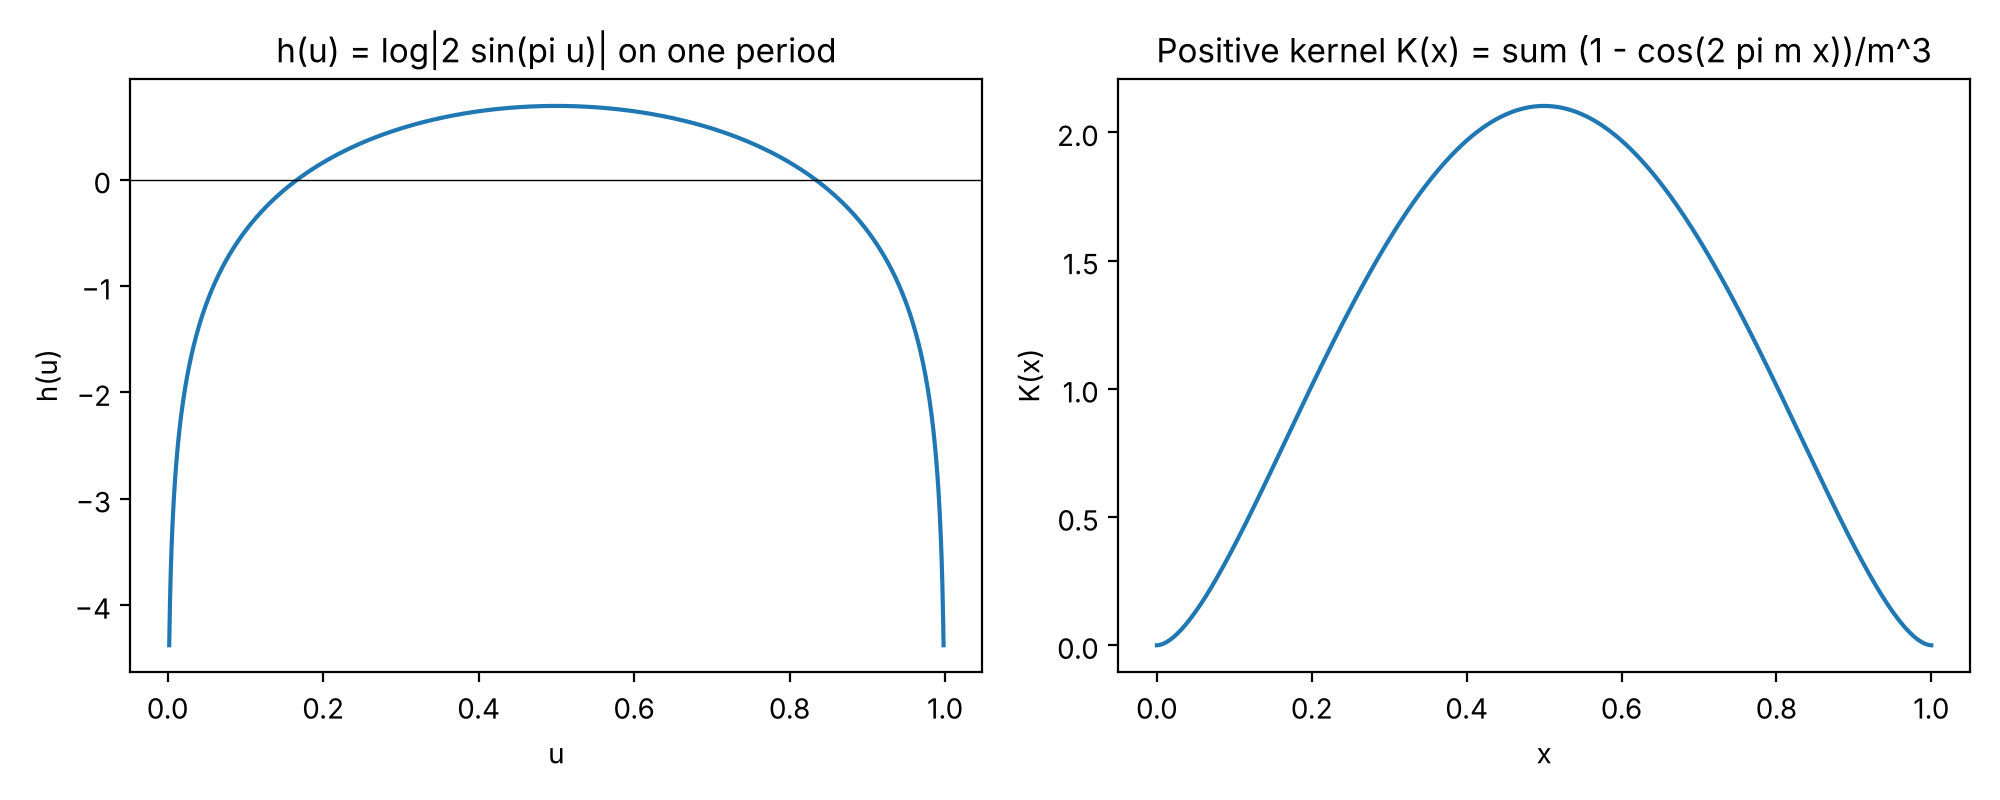
\includegraphics[width=0.95\textwidth]{fig_kernel.png}
\caption{The function $h$ on one period and the positive kernel $\mathcal K$.}\label{fig:kernel}
\end{figure}

\begin{figure}[ht]
\centering
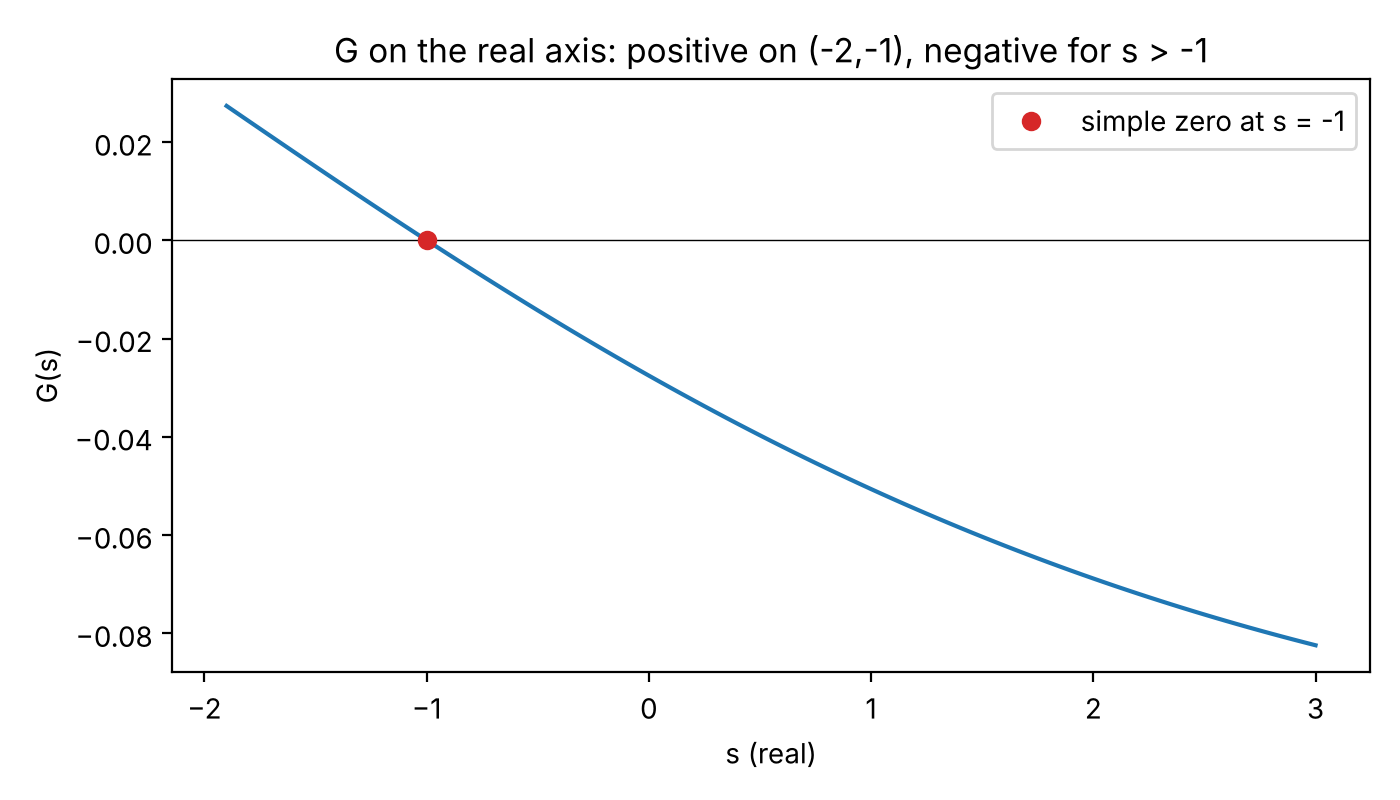
\includegraphics[width=0.7\textwidth]{fig_G_real.png}
\caption{$G$ on the real axis.}\label{fig:Greal}
\end{figure}

\begin{figure}[ht]
\centering
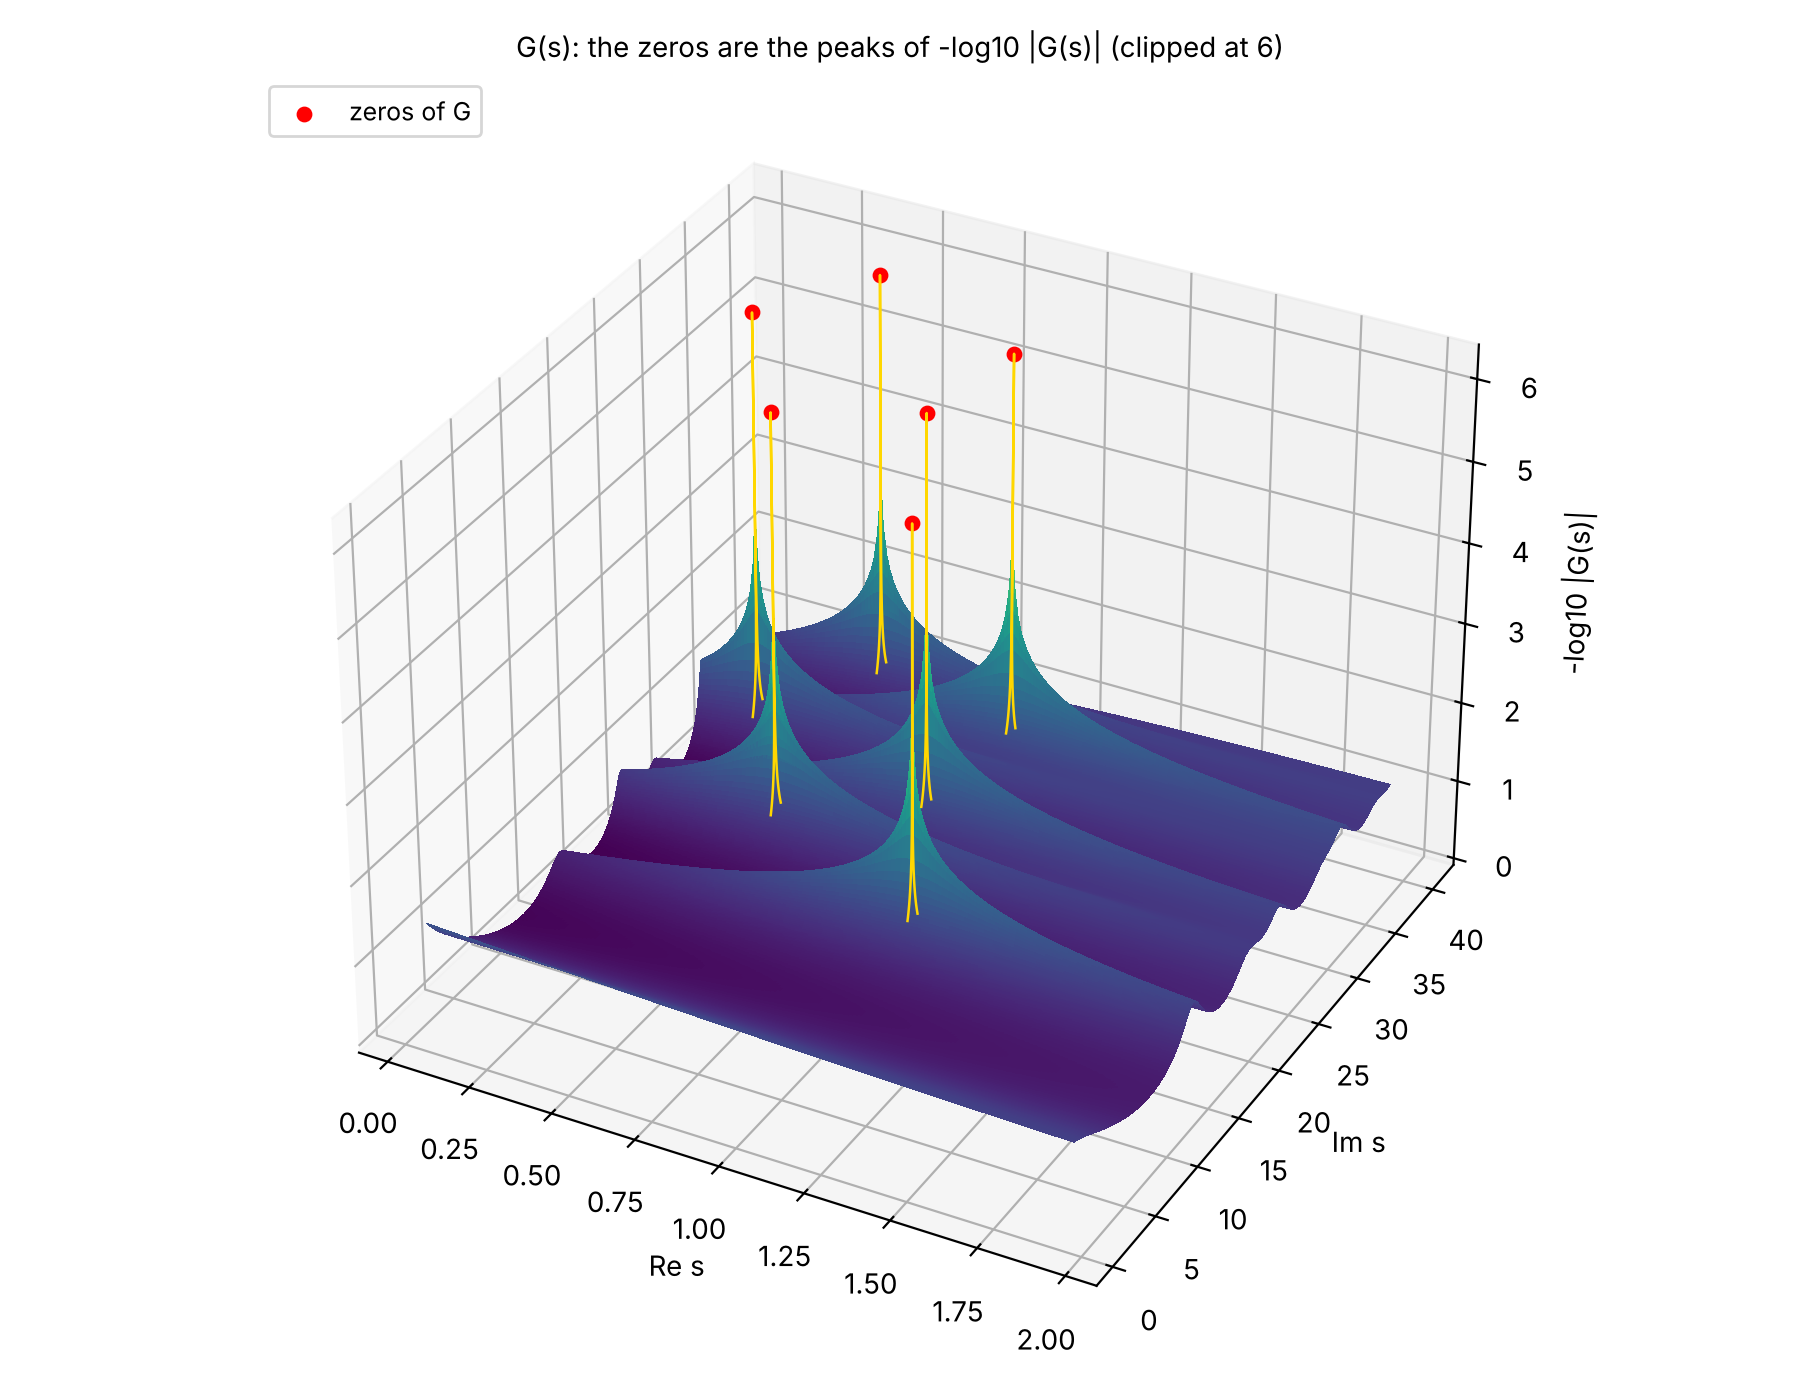
\includegraphics[width=0.8\textwidth]{fig_G_surface.png}
\caption{$-\log_{10}|G(s)|$, clipped at $6$. The peaks are the six zeros of $G$ of Table~\CGref{tab:rouche}.}\label{fig:Gsurf}
\end{figure}

\begin{figure}[ht]
\centering
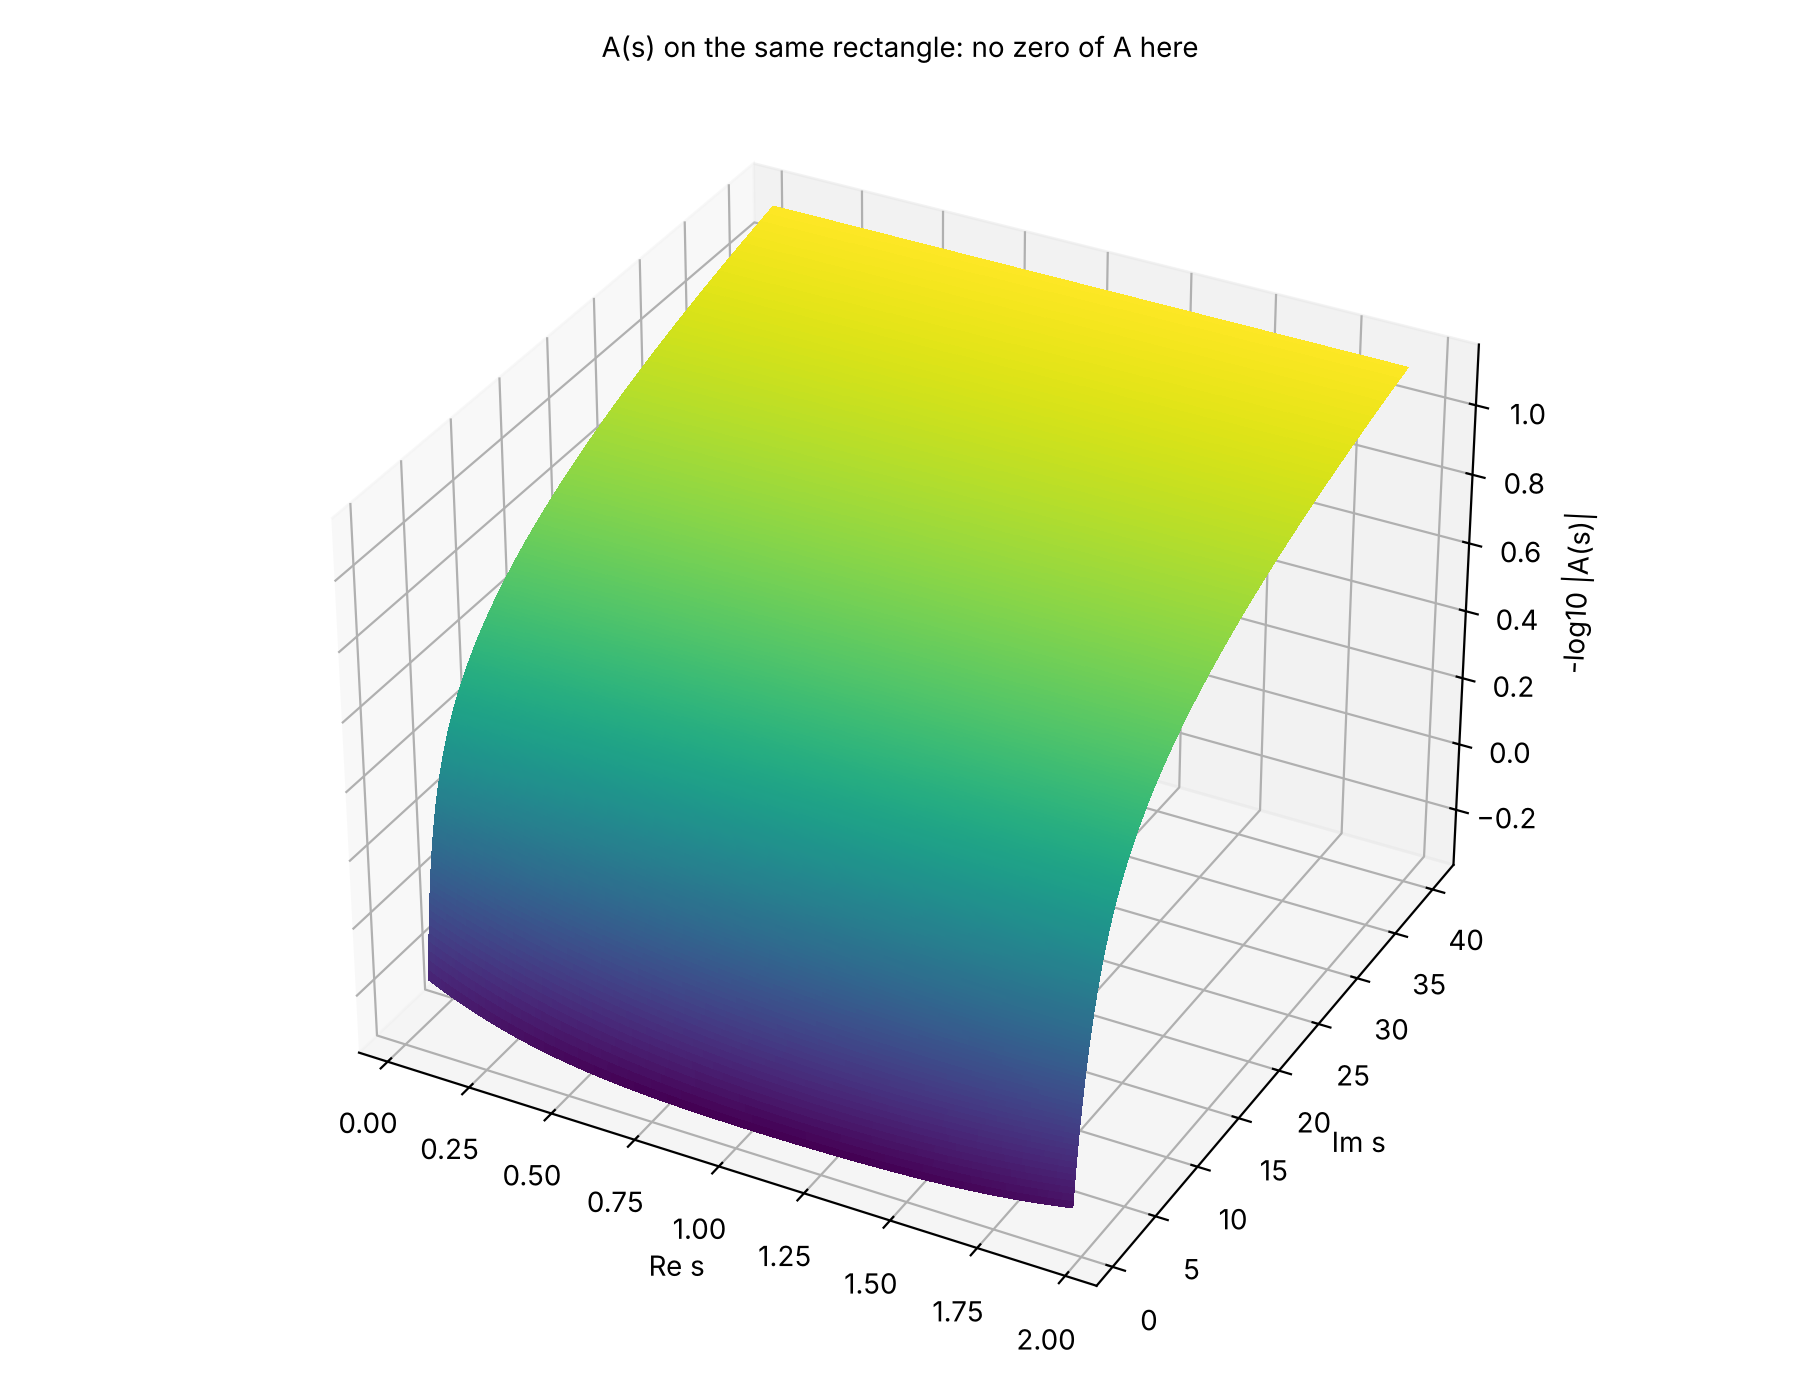
\includegraphics[width=0.8\textwidth]{fig_A_surface.png}
\caption{$-\log_{10}|A(s)|$ on the rectangle of Figure~\CGref{fig:Gsurf}.}\label{fig:Asurf}
\end{figure}

\begin{figure}[ht]
\centering
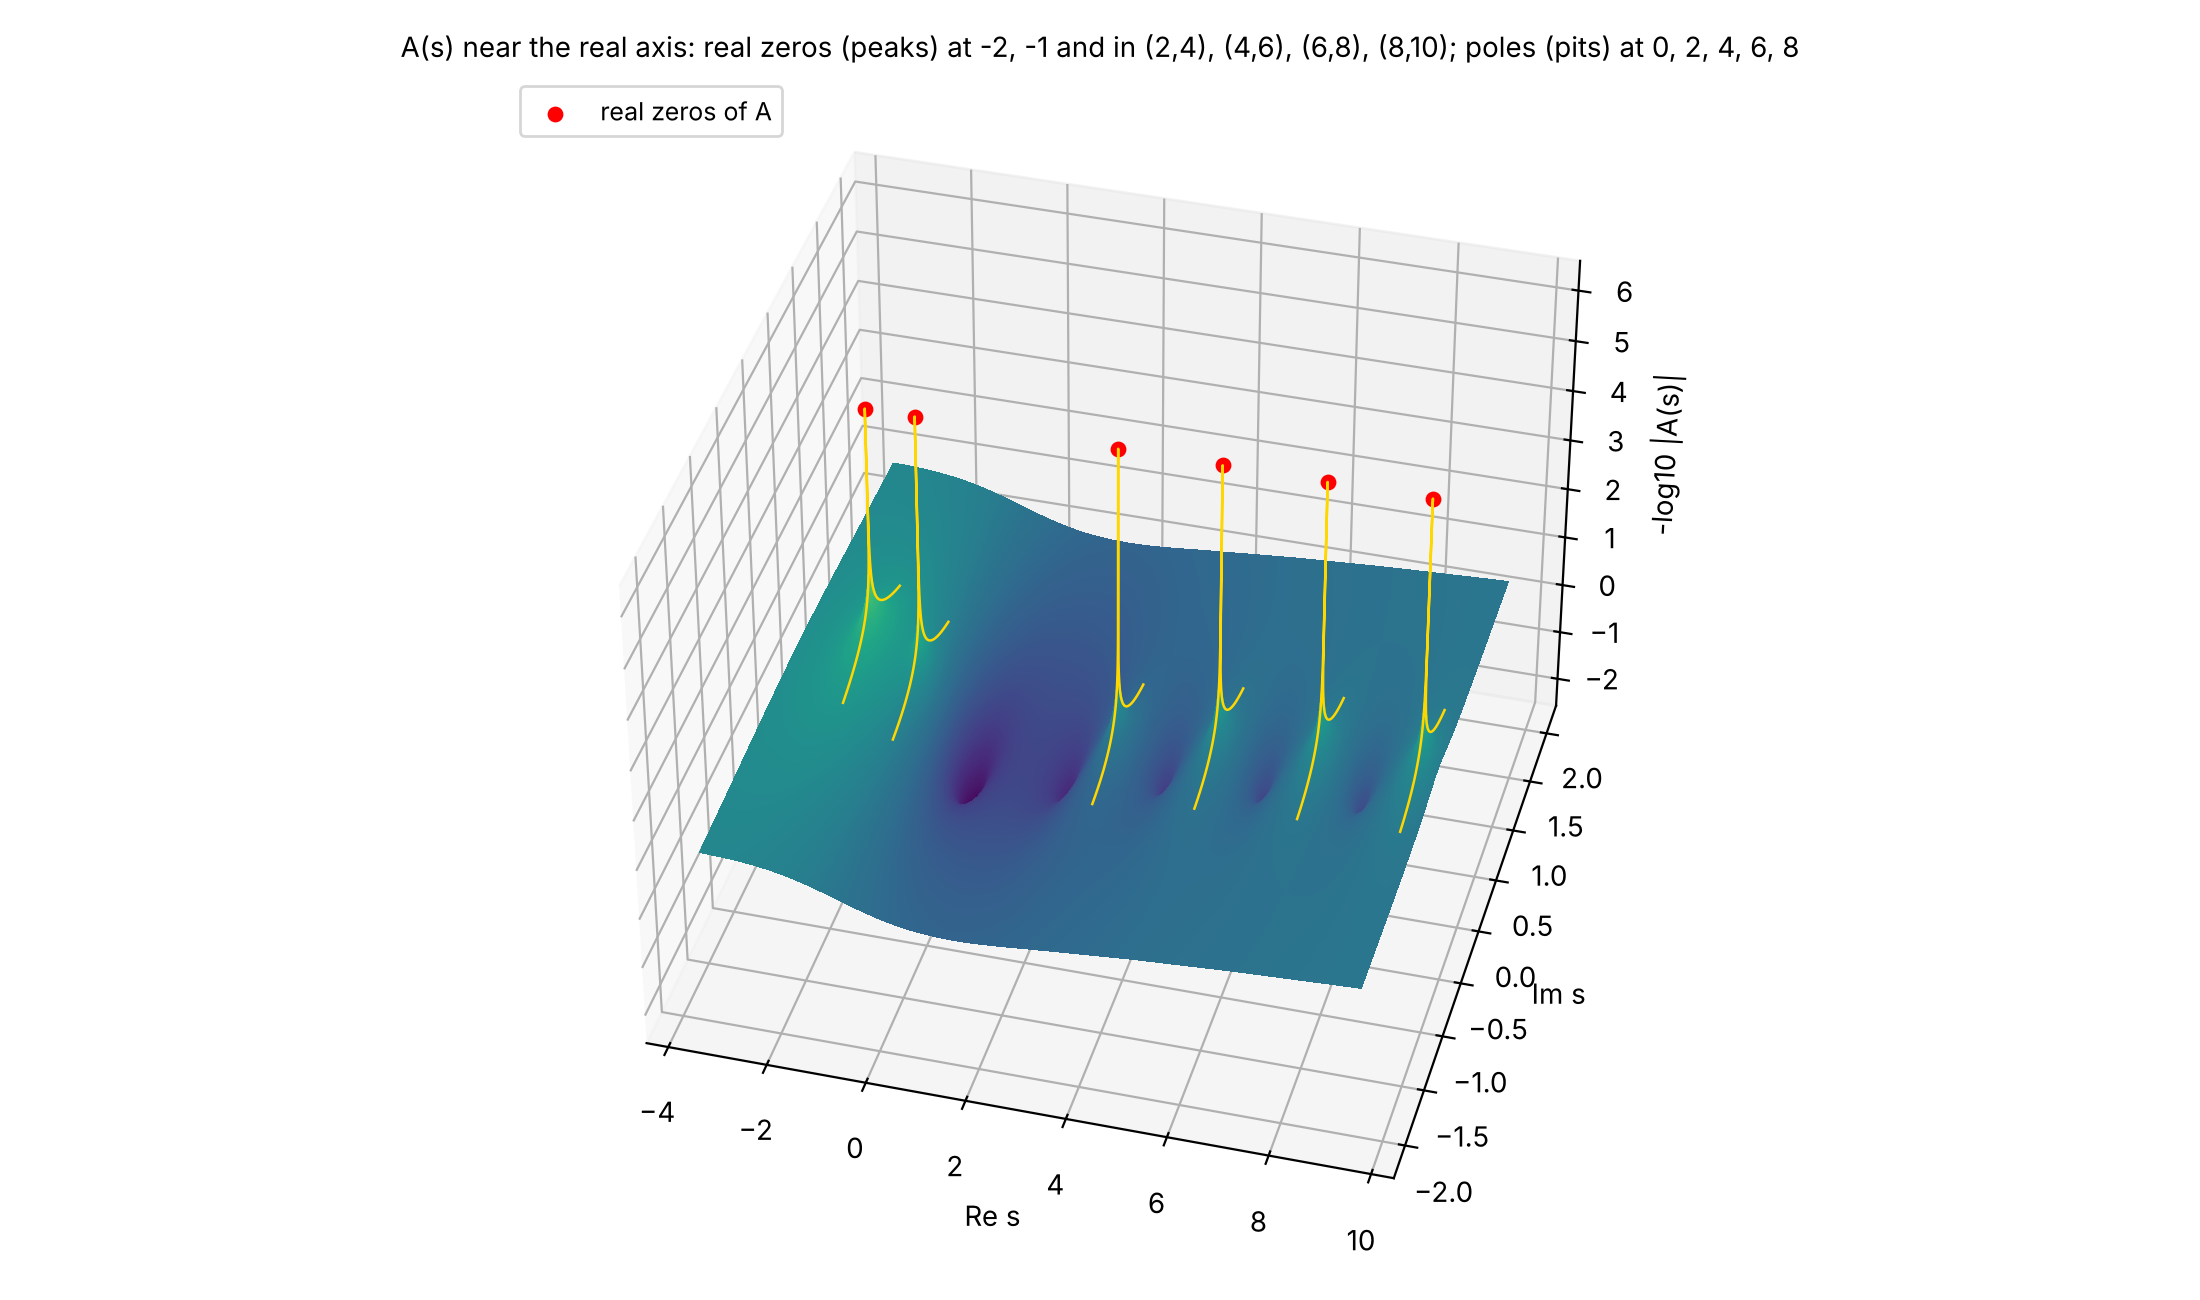
\includegraphics[width=0.95\textwidth]{fig_A_real_surface.png}
\caption{$-\log_{10}|A(s)|$ near the real axis, clipped to $[-2,6]$. The peaks are real zeros of $A$ and the pits are its poles at $0,2,4,6,8$.}\label{fig:Areal}
\end{figure}

\begin{figure}[ht]
\centering
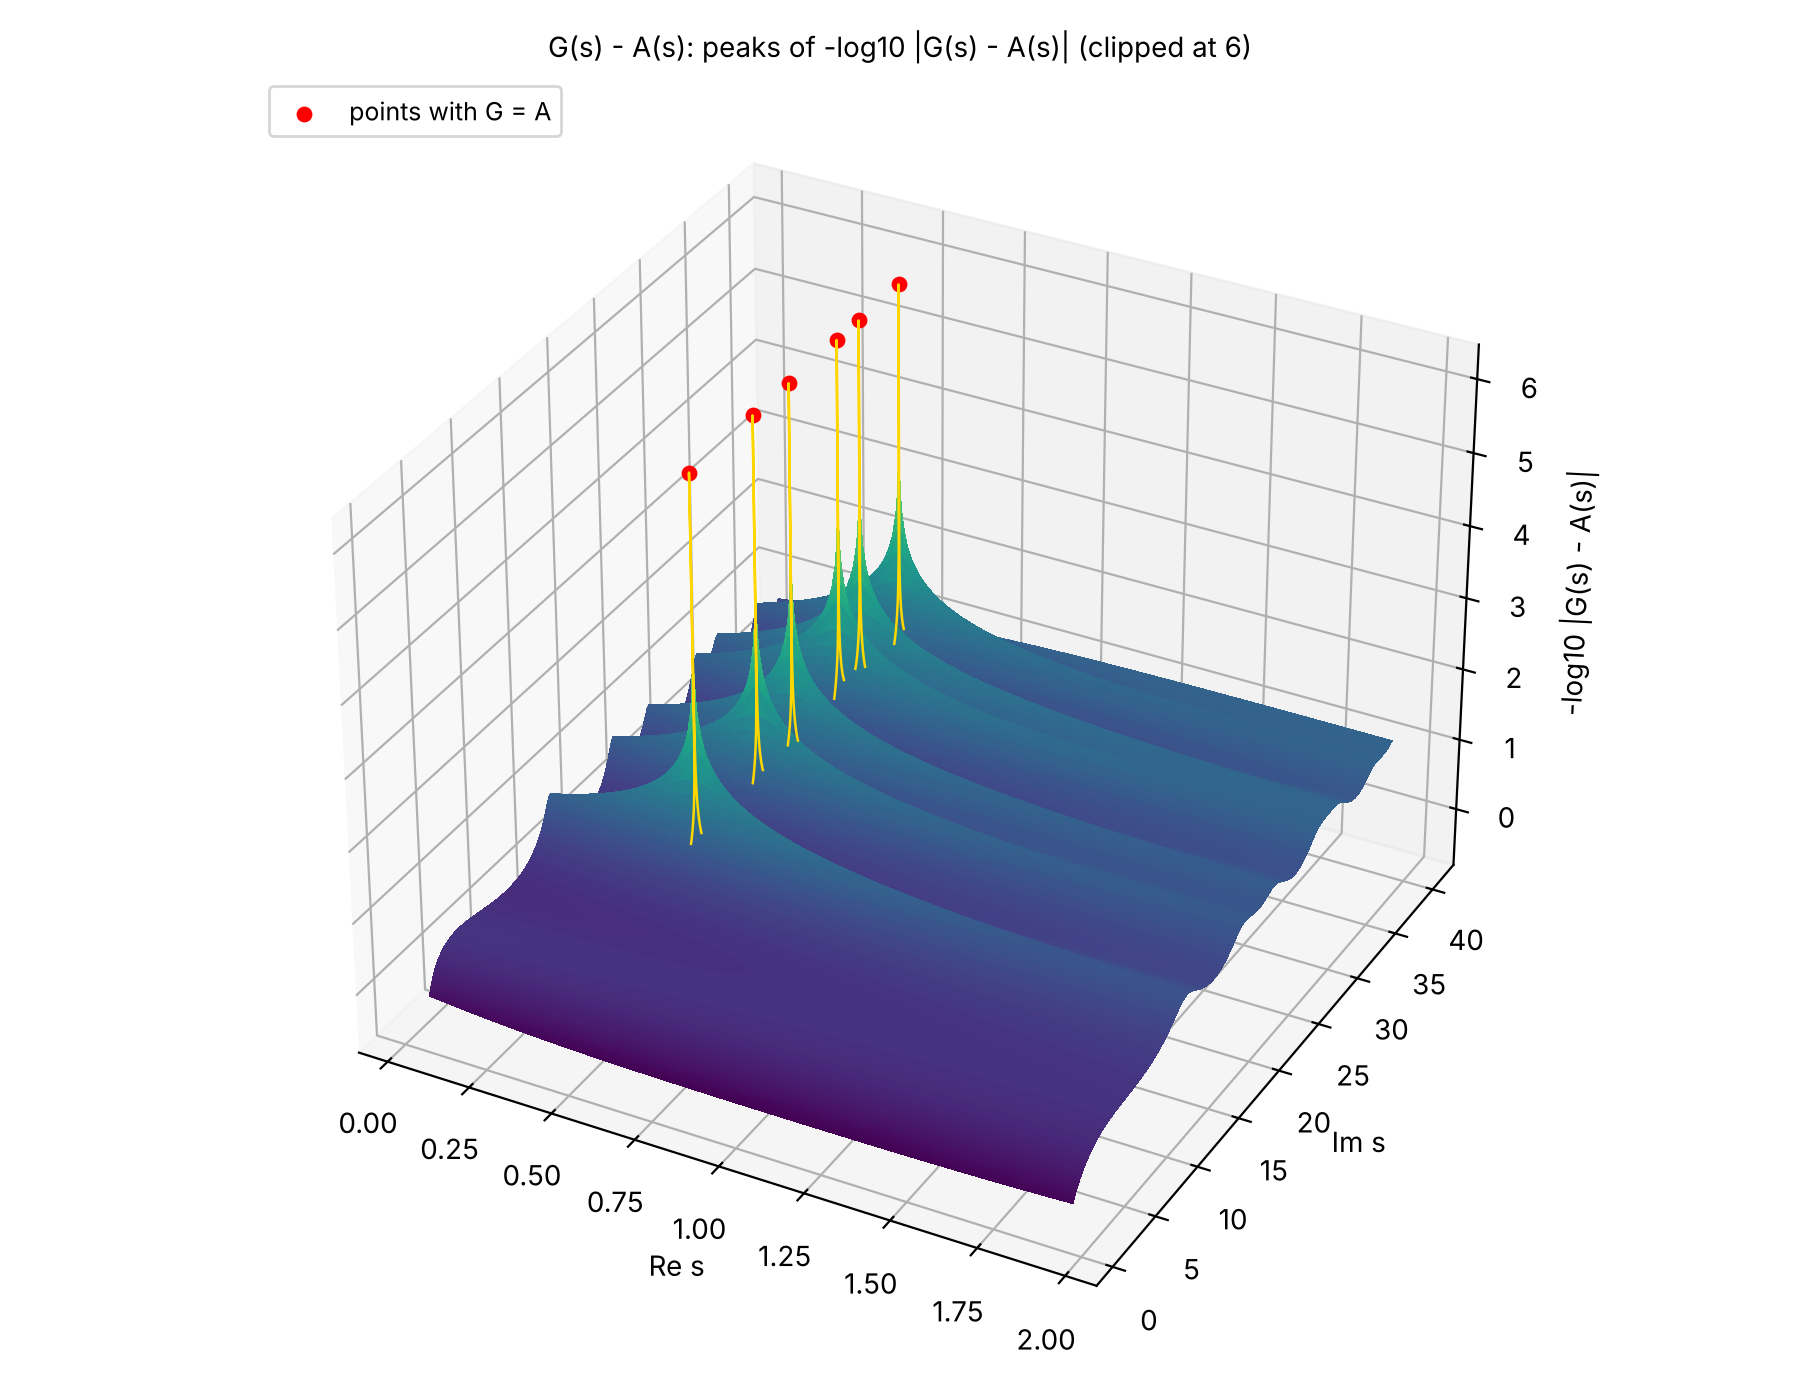
\includegraphics[width=0.8\textwidth]{fig_GminusA_surface.png}
\caption{$-\log_{10}|G(s)-A(s)|$, clipped at $6$. The peaks are at the six points $\frac12+it$ of Figure~\CGref{fig:zeromap}.}\label{fig:GAsurf}
\end{figure}

\begin{figure}[ht]
\centering
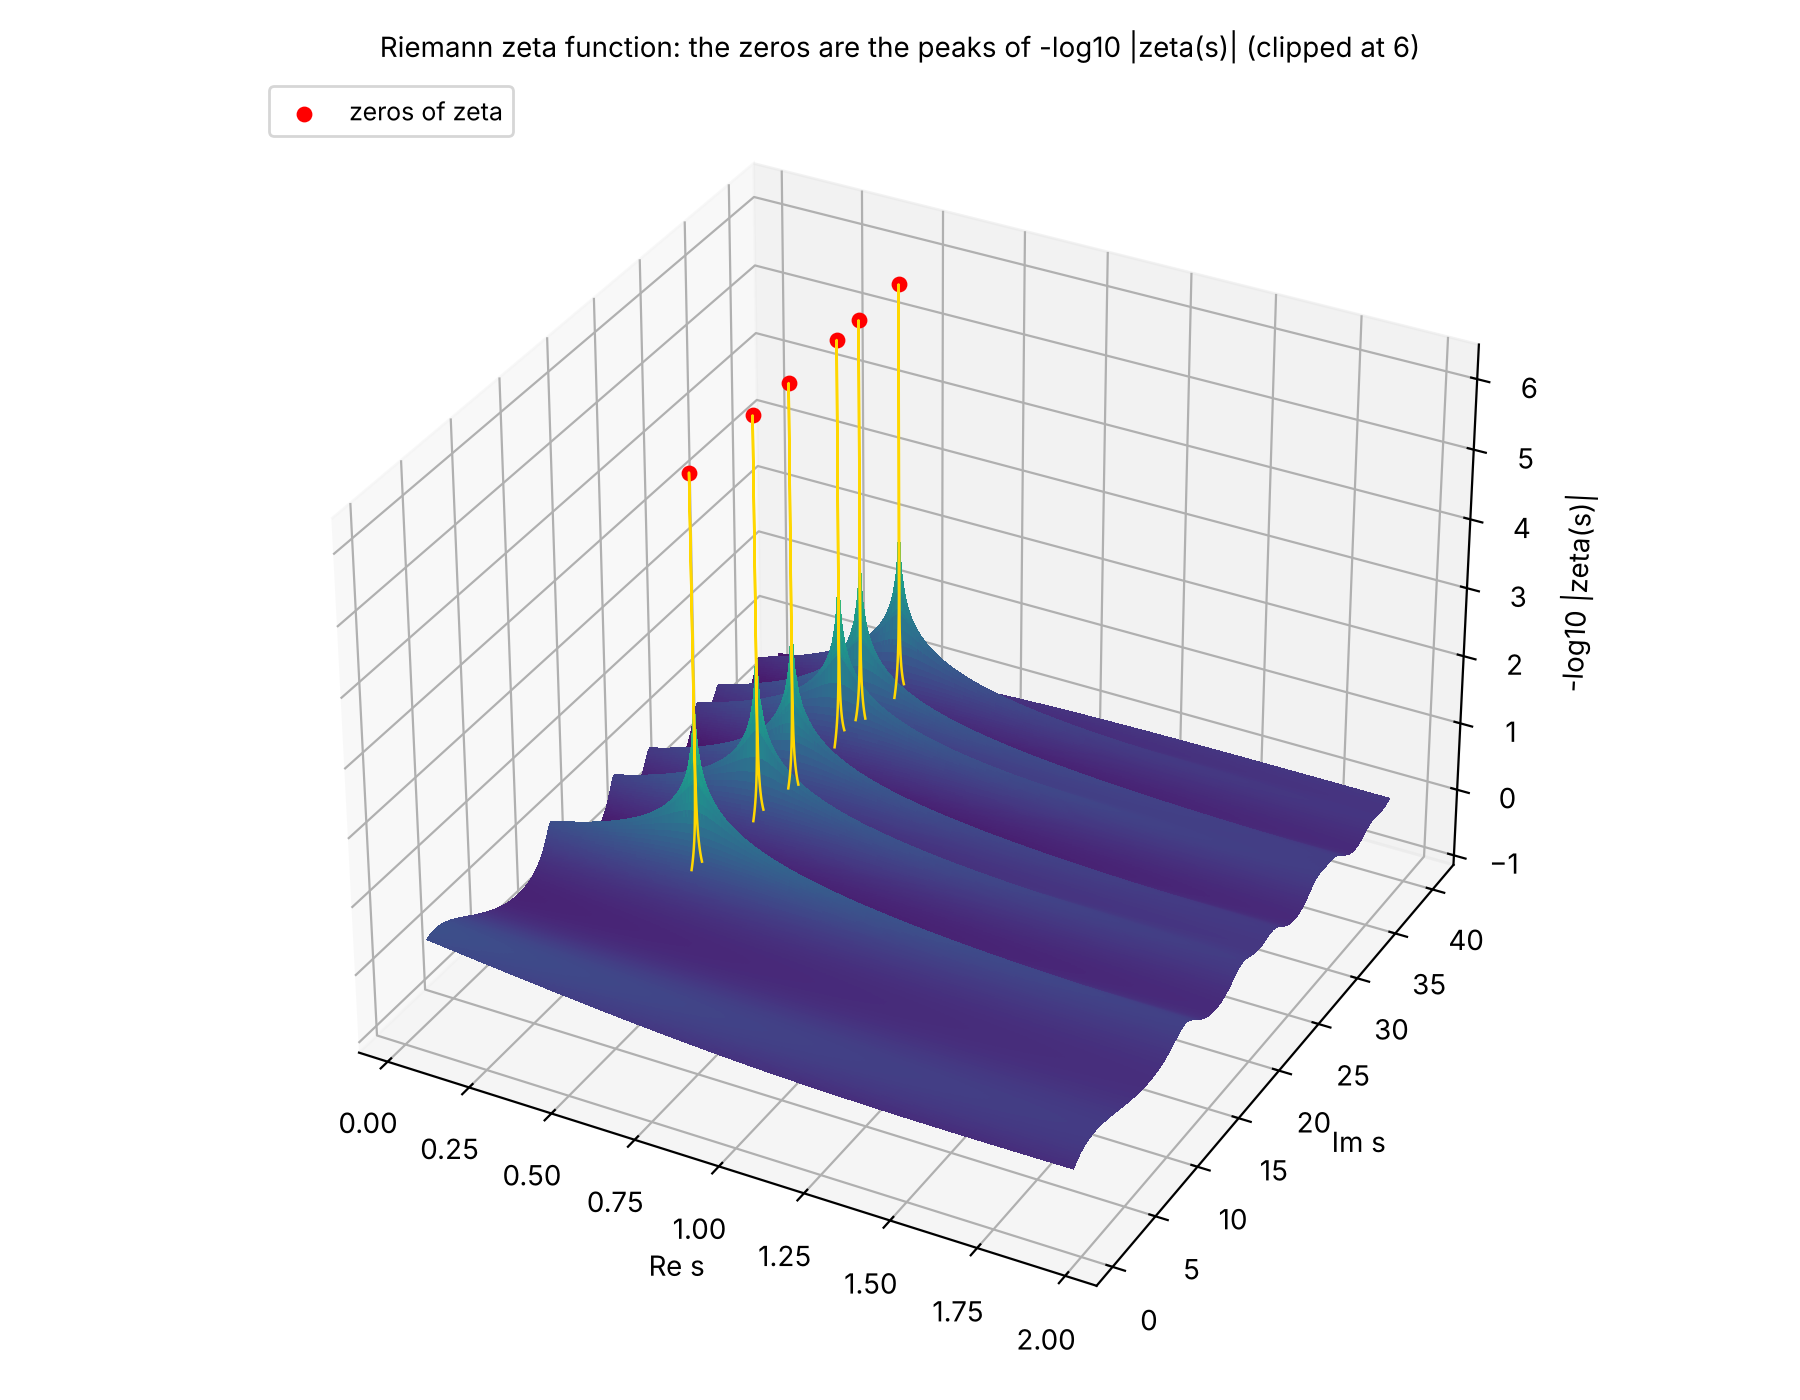
\includegraphics[width=0.8\textwidth]{fig_zeta_surface.png}
\caption{$-\log_{10}|\zeta(s)|$, clipped at $6$. The peaks are the first six nontrivial zeros of $\zeta$.}\label{fig:zetasurf}
\end{figure}

\begin{figure}[ht]
\centering
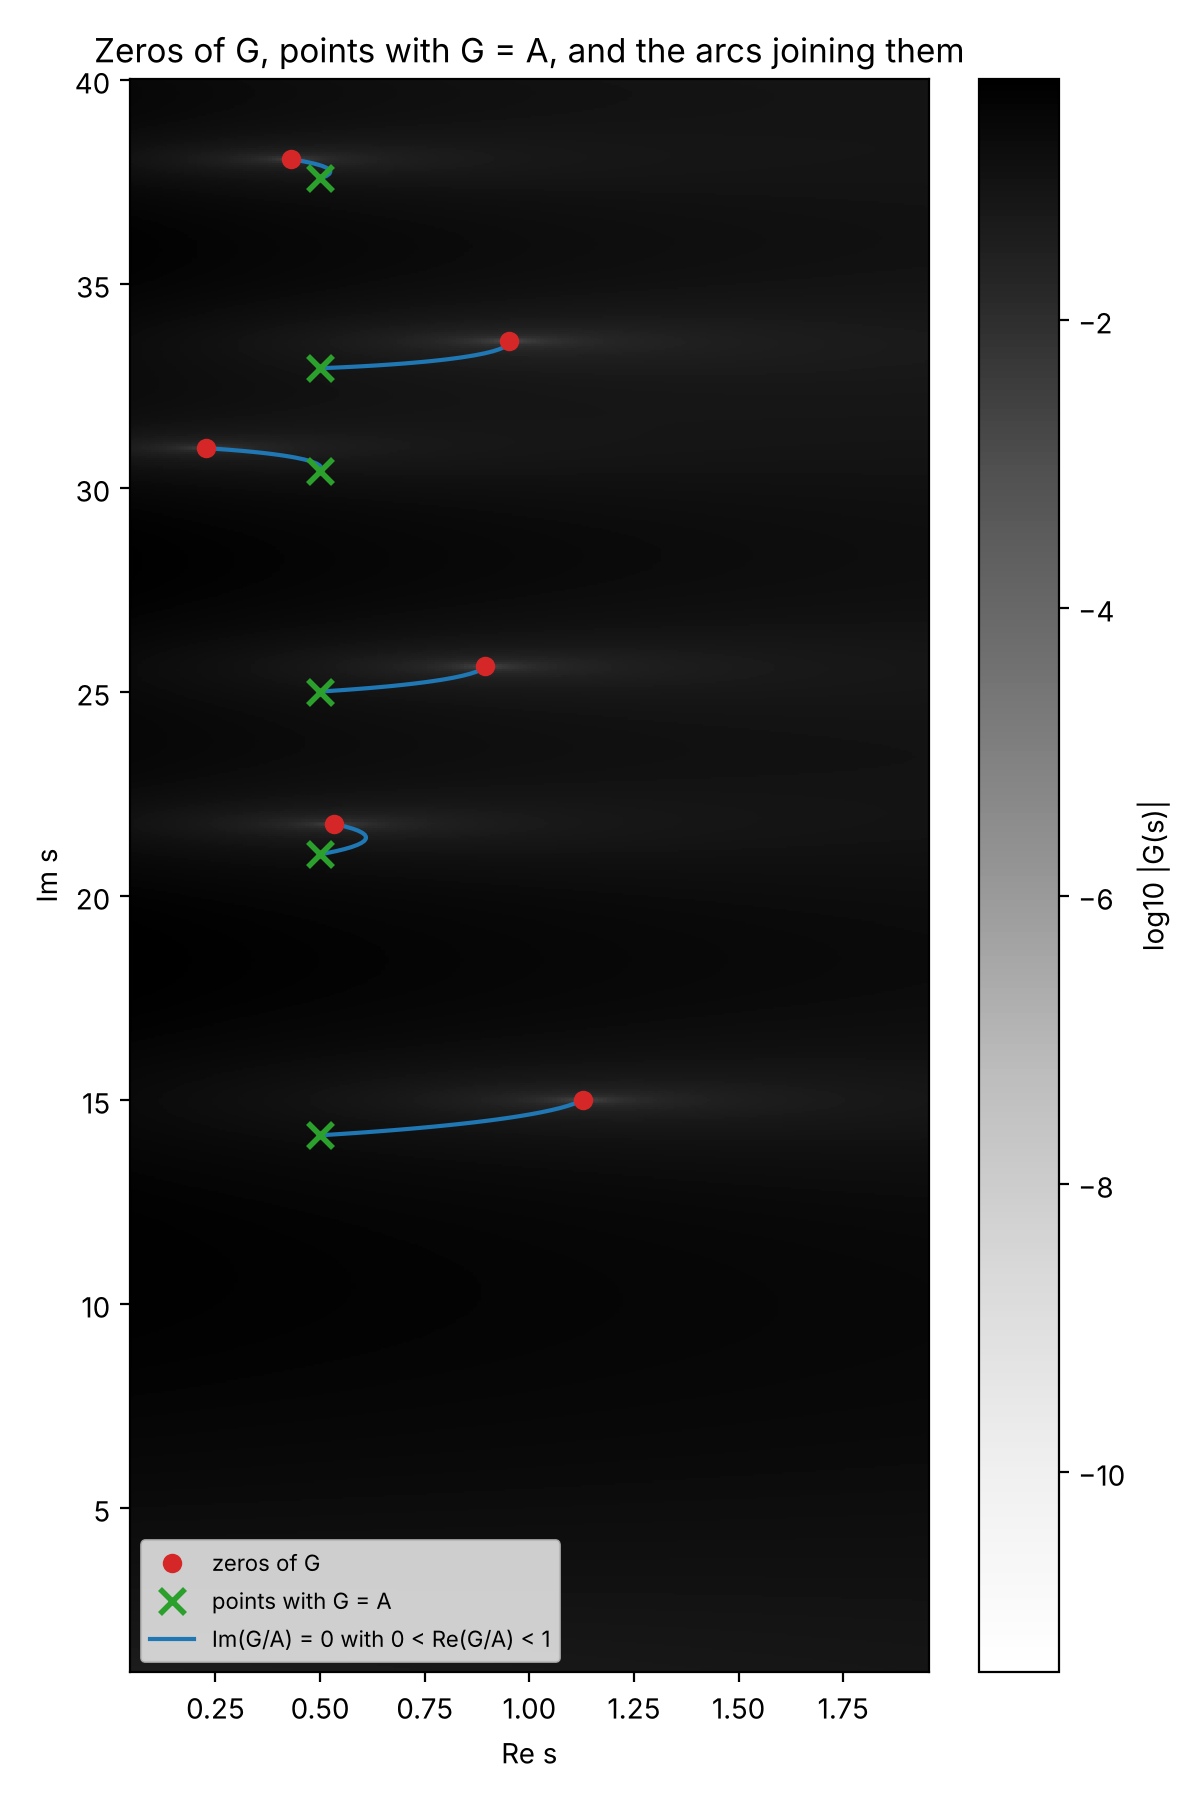
\includegraphics[width=0.6\textwidth]{fig_zero_map.png}
\caption{Computed zeros of $G$, computed points with $G=A$, and the computed arcs of $\operatorname{Im}(G/A)=0$ with $0<\operatorname{Re}(G/A)<1$, at points where $A\ne0$. The pairing shown by the arcs is a numerical observation.}\label{fig:zeromap}
\end{figure}

\begin{figure}[ht]
\centering
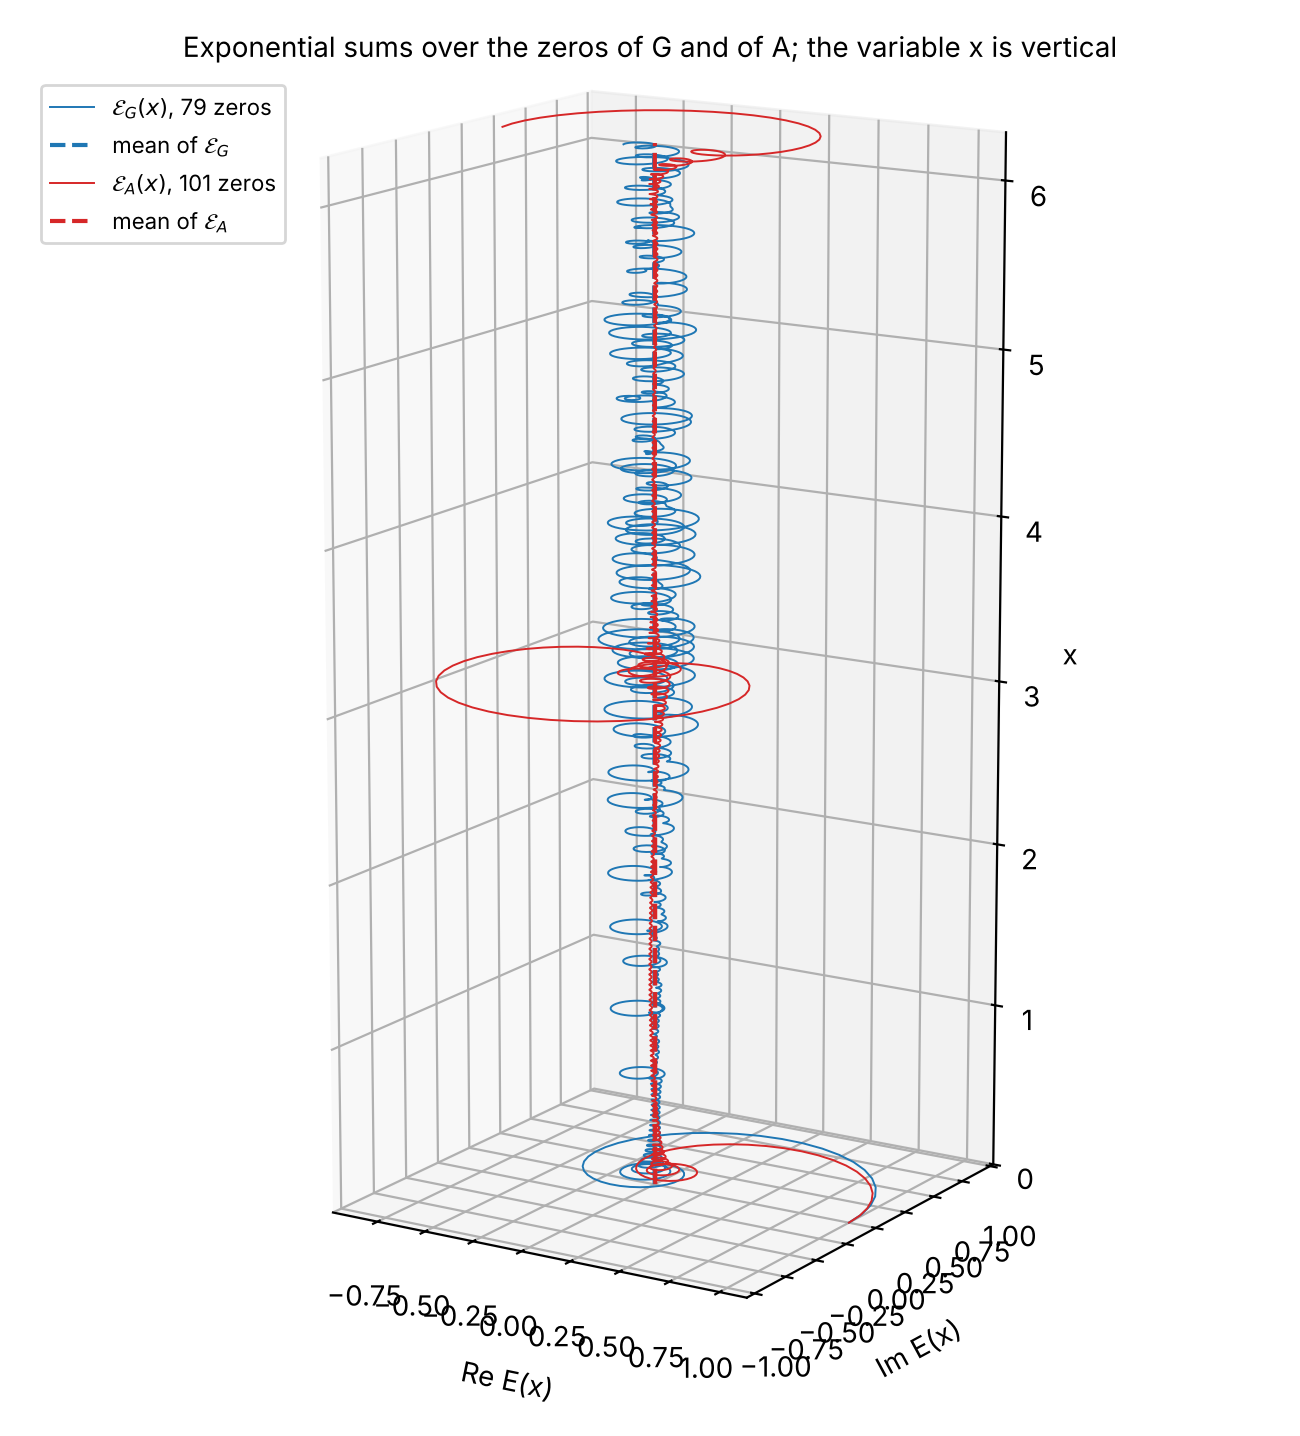
\includegraphics[width=0.55\textwidth]{fig_expsum_3d.png}
\caption{The exponential sums $\mathcal E_G(x)$ and $\mathcal E_A(x)$ of \CGeqref{eq:expsum} for $0\le x\le2\pi$. The variable $x$ is the vertical axis. The dashed lines are the means of the two curves.}\label{fig:expsum3d}
\end{figure}

\begin{figure}[ht]
\centering
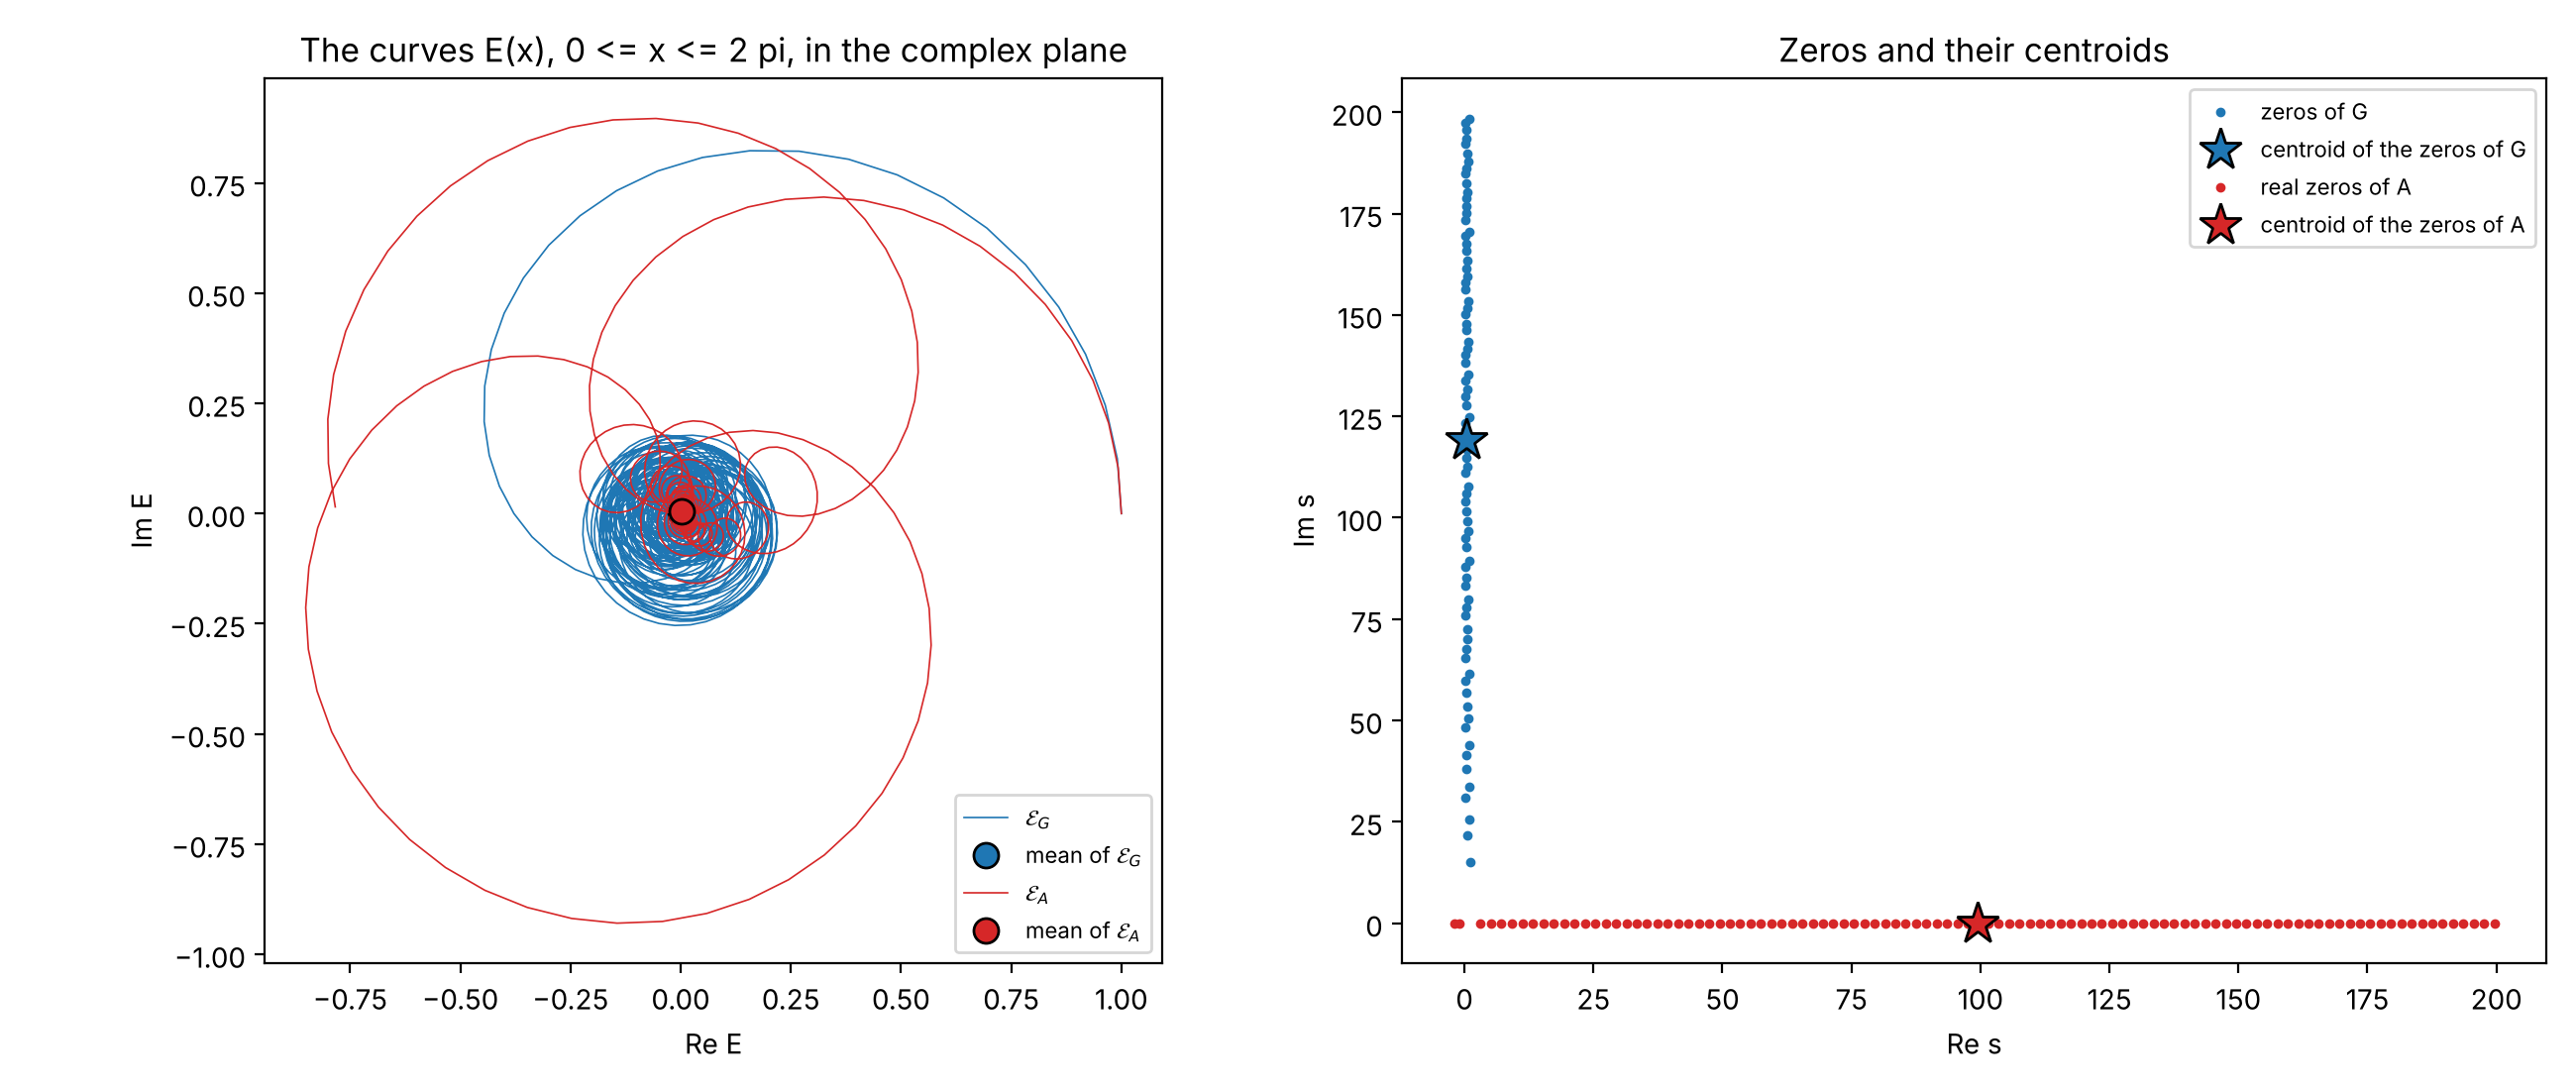
\includegraphics[width=0.98\textwidth]{fig_expsum_plane.png}
\caption{Left: the curves $\mathcal E_G$ and $\mathcal E_A$ in the complex plane. Right: the $79$ computed zeros of $G$ and the $101$ computed real zeros of $A$, with their centroids.}\label{fig:expsumplane}
\end{figure}

\begin{figure}[ht]
\centering
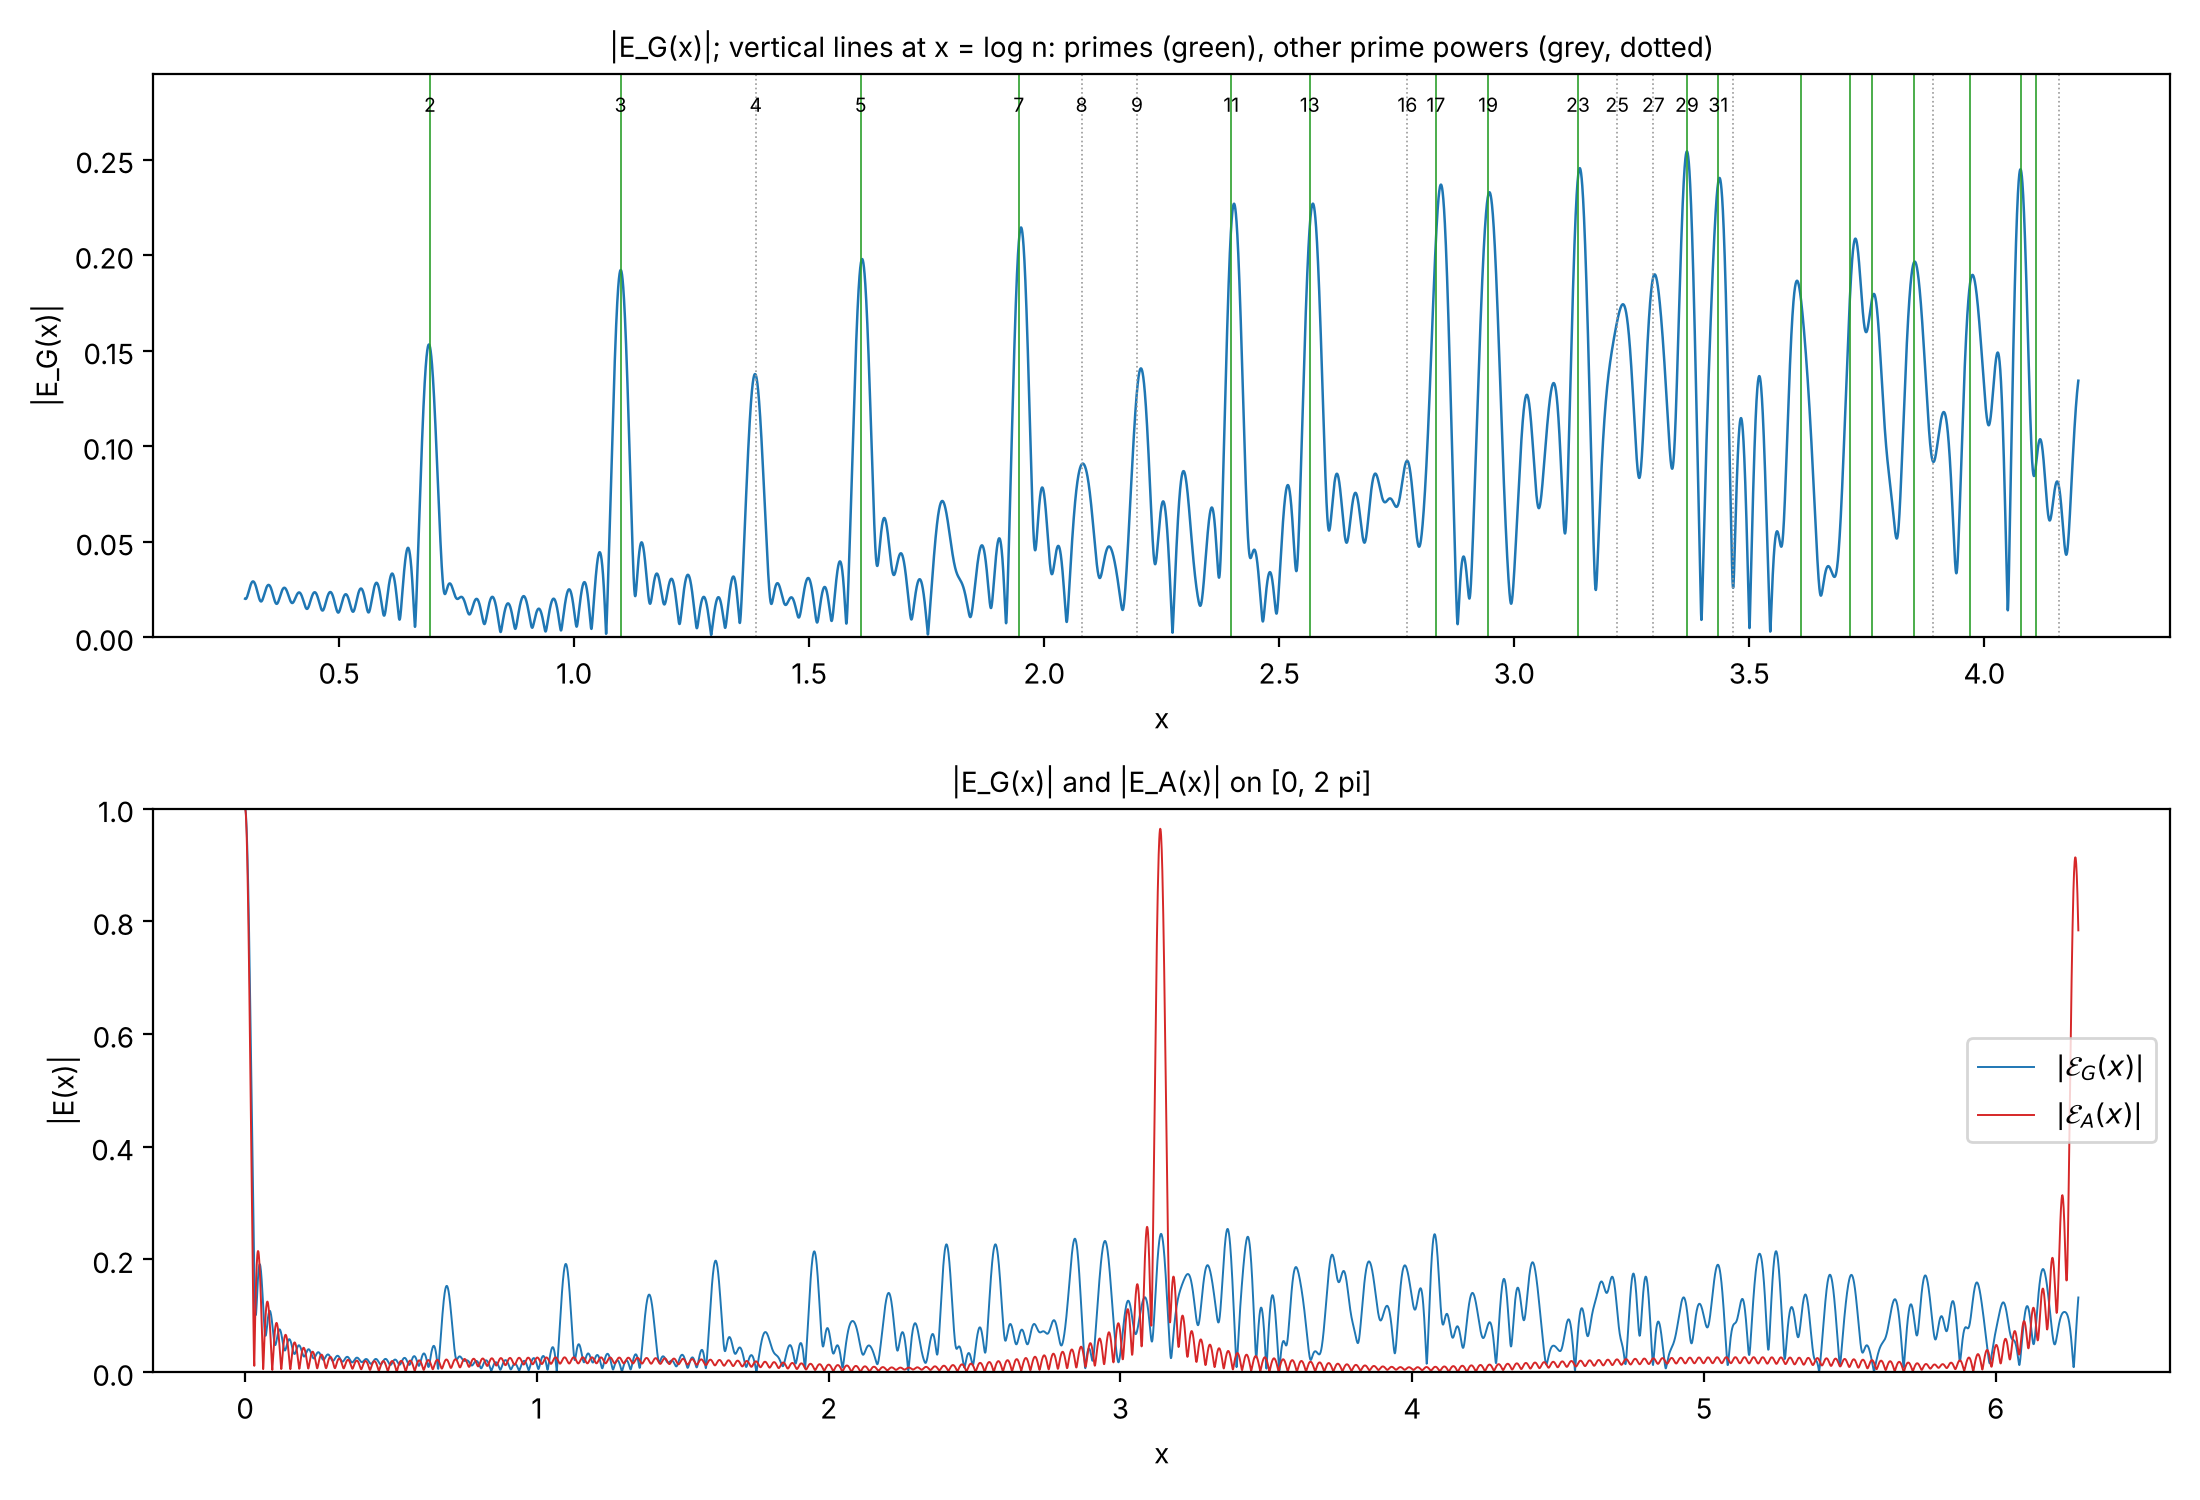
\includegraphics[width=0.95\textwidth]{fig_expsum_modulus.png}
\caption{Top: $|\mathcal E_G(x)|$ for $0.3\le x\le4.2$, with vertical lines at $x=\log n$ for the prime powers $n\le66$. Bottom: $|\mathcal E_G(x)|$ and $|\mathcal E_A(x)|$ for $0\le x\le2\pi$.}\label{fig:expsummod}
\end{figure}

\begin{figure}[ht]
\centering
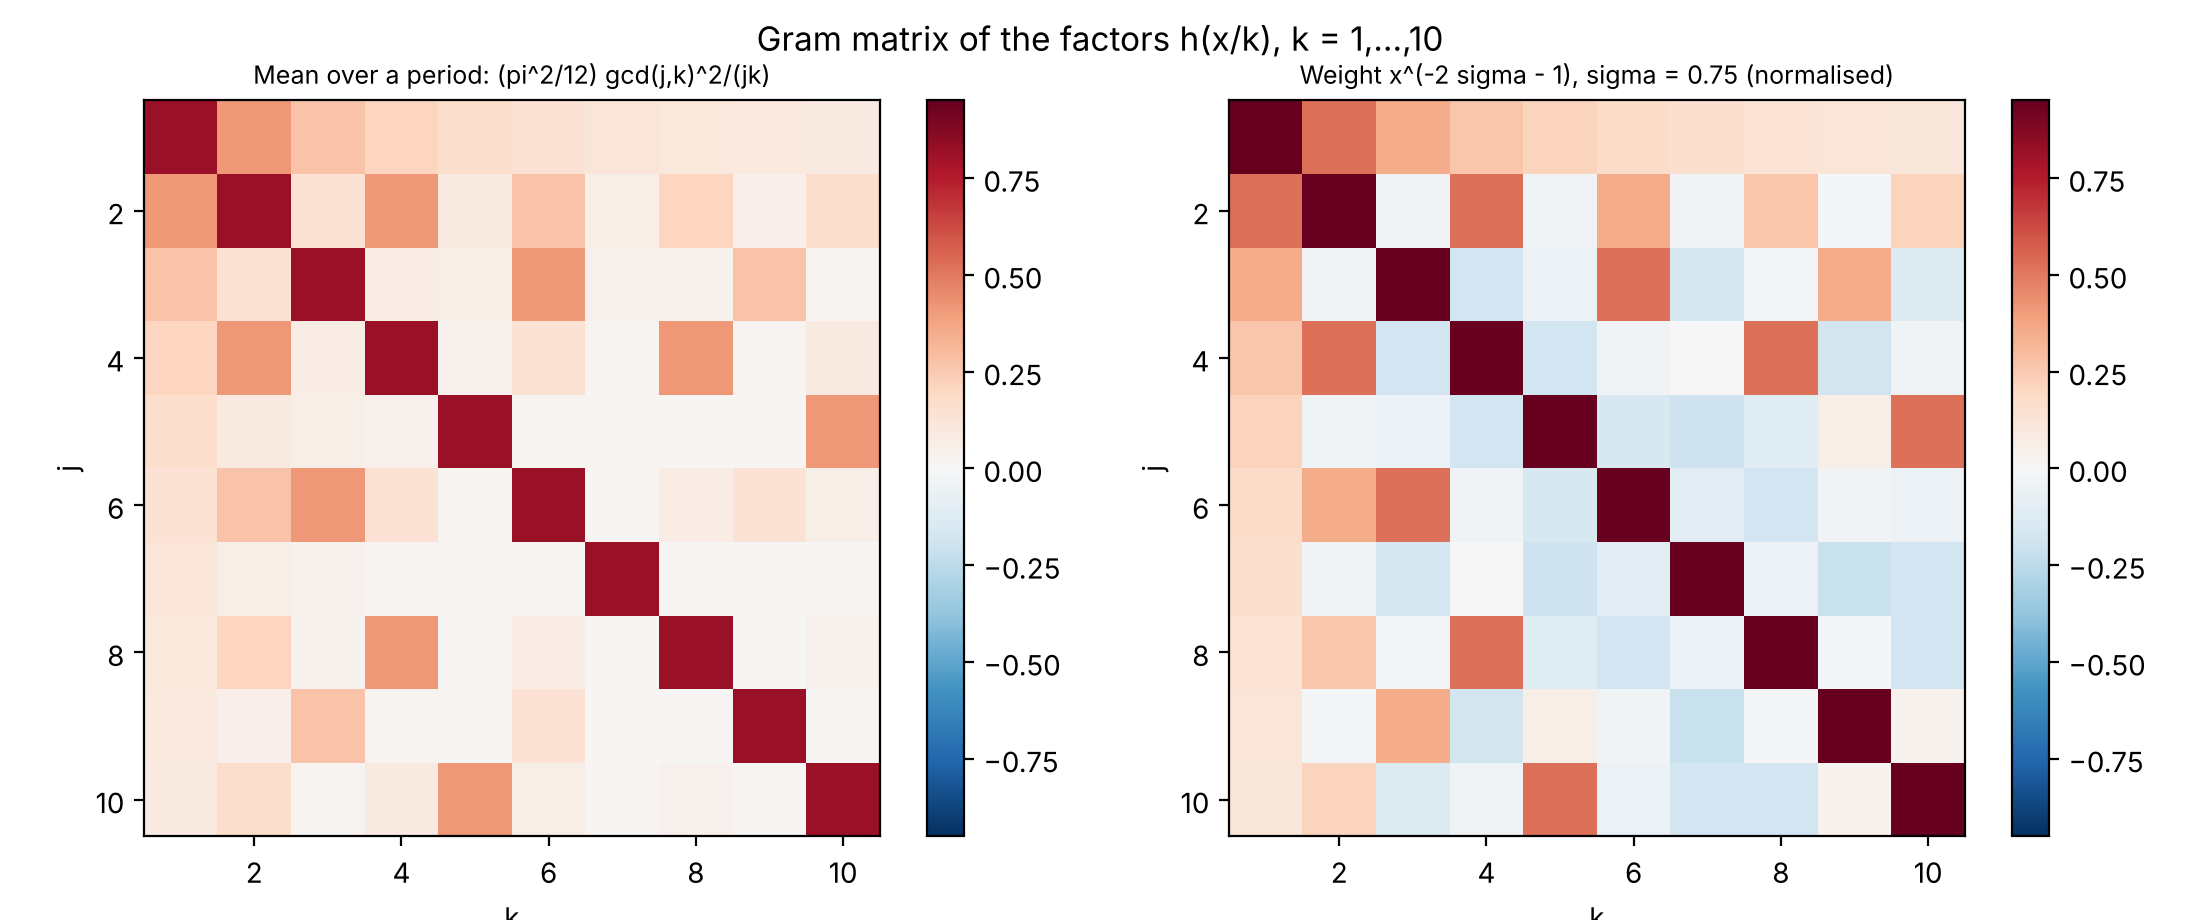
\includegraphics[width=0.98\textwidth]{fig_gram.png}
\caption{Gram matrices of the factors $h(x/k)$, $1\le k\le10$: mean over a period, and weight $x^{-2\sigma-1}$ with $\sigma=\frac34$.}\label{fig:gram}
\end{figure}

\clearpage
\begin{thebibliography}{9}

\bibitem{Johansson2017}
F.~Johansson, Arb: efficient arbitrary-precision midpoint-radius interval arithmetic, \emph{IEEE Trans. Comput.} \textbf{66} (2017), no.~8, 1281--1292.
\href{https://doi.org/10.1109/TC.2017.2690633}{doi:10.1109/TC.2017.2690633}.

\bibitem{Smith1875}
H.~J.~S.~Smith, On the value of a certain arithmetical determinant, \emph{Proc. London Math. Soc.} \textbf{7} (1875/76), 208--212.
\href{https://doi.org/10.1112/plms/s1-7.1.208}{doi:10.1112/plms/s1-7.1.208}.

\end{thebibliography}

\end{document}

# BEGIN CORRECTVCG  (CorrectVCG checker, ignored by LaTeX; extract with the sed line at the top)
#!/usr/bin/env python3
r"""CorrectVCG checker (version 10) for Doktor's manuscripts and for Theorems and Proofs (TP).

Every .tex delivered to him carries a copy of this script after \end{document} (LaTeX never reads it).
Extract it with:   sed -n '/^# BEGIN CORRECTVCG/,/^# END CORRECTVCG/p' FILE.tex > correctvcg_check.py
Read every rule first:   python3 correctvcg_check.py --rules
Main uses:
    python3 correctvcg_check.py --paper FILE.tex                      format + mathematical checks of a manuscript
    python3 correctvcg_check.py CHAPTER.tex --chapter N --previous OLD  TP chapter
    python3 correctvcg_check.py --paper NEW.tex --diff OLD.tex --allowed labels.txt   no unrequested change
    python3 correctvcg_check.py FILE.tex --mark OUT.tex               review marks \VCGreviewed{n}
    python3 correctvcg_check.py FILE.tex --mark OUT.tex --reviewer codex     Codex marks \VCGreviewedCodex{n}
    python3 correctvcg_check.py FILE.tex --mark OUT.tex --reviewer chatgpt   ChatGPT marks \VCGreviewedChatGPT{n}
    python3 correctvcg_check.py FILE.tex --mark OUT.tex --reviewer copilot   Copilot marks \VCGreviewedCopilot{n}
    python3 correctvcg_check.py FILE.tex --embed OUT.tex              put this checker into a .tex
Exit code 0 only if there are no ERROR lines.  WARN lines must be read and fixed or justified one by one.
"""
import re
import sys
import argparse
import os
from collections import Counter

RULES = r'''
CorrectVCG RULES (v5). Every correction Doktor (Victor Casana-Giner) has had to make, mathematical and formal.
They apply to ALL his papers, notes, reviews and to every chapter of the book Theorems and Proofs (TP), not to one paper.
Read all of them before touching any of his .tex files. The past cases behind each rule are listed (in Spanish) in the
project docs claude/CorrectVCG-errores-matematicos-v4.md, claude/CorrectVCG-formato-v2.md, claude/CorrectVCG-listado-correcciones-v1.md.
This block and the checker below travel inside every .tex after \end{document}. NEVER remove them automatically:
they are removed only when Doktor himself asks for it (final versions).

RULE ZERO. Every error in what I deliver is mine, wherever it came from (source, other author, other AI, one of his drafts).
"It came from the source" is never an excuse.

THE NINE PATTERNS I REPEAT (check each one, in writing, before delivering anything):
 1. Marking a point as corrected without looking at the final output.
 2. Not running through the boundary cases: 0, negative values, 1, the first value of every index, empty ranges, degenerate parameters, the sign when dividing.
 3. Leaving symbols undefined, without domain, used before being defined, with two meanings, or renamed in only part of the text.
 4. Writing "equivalent", "suffices", "necessary", "unconditional" without both directions or the quantitative form.
 5. Leaving hard steps as "the same argument", "applies verbatim", "similarly", "as in [ref]".
 6. Marking a statement as verified without redoing the computations.
 7. Ignoring corrections he already gave: before delivering, run through all the accumulated rules.
 8. Fixing only the first occurrence of an error (first paragraph or section) and not the others.
 9. Importing results and errors from his papers and drafts without re-proving them, or citing him in the bibliography.
 And the one that annoys him most: in a revision, changing things that were right and breaking them. Only what he asks, or a proven error, changes; everything else stays letter by letter (checker: --diff OLD --allowed labels.txt).

ONE COMPLETE REVIEW SHOULD SUFFICE. Every review is complete, as if it were the only one: every statement, the whole checklist
below on each, every occurrence of every error, checker with 0 ERROR. In practice there will be several; none relaxes anything.
Every reviewed statement carries the reviewer's own mark in the LaTeX (n = number of reviews of that statement by that reviewer;
checker --mark --reviewer R): Claude \VCGreviewed{n}, Codex \VCGreviewedCodex{n}, ChatGPT \VCGreviewedChatGPT{n},
Copilot \VCGreviewedCopilot{n}.
Each reviewer touches only its own marks; the marks, counters and preamble block of the other reviewers stay letter by letter
(checker --diff gives ERROR otherwise). Review marks are not text changes and are ignored by every content check and by the
unrequested-change check. The embedded checker is never replaced by an older version (--embed refuses), and never removed unless
Doktor asks.

A. WHAT IS ASKED, AND APPLYING A CORRECTION REPORT
 A1. Deliver exactly the object asked (a chapter of TP is a chapter of TP, not a new version of its source paper; "only that part" means nothing else). A new version of a paper or of TP only when he asks.
 A2. If object or scope is unclear, ask ONCE before generating. Never regenerate "just in case".
 A3. For every report: point -> cause (mathematics / generator / text) -> where it is fixed -> LITERAL QUOTE of the corrected text in the FINAL OUTPUT. A point without that quote is not corrected.
 A4. Every correction in all its occurrences: grep the error and its variants (same symbol, formula, phrase, copies in settings, tooltips, abstract, introduction, other sections, other chapters, the checker, the skill); count before, 0 after. A general correction becomes a global convention, and every place that depended on it is revisited.
 A5. Never mark corrections as applied in block; each one is checked in the output.
 A6. Regression: in every new version re-check ALL points of ALL previous rounds.
 A7. If a report flags some cases of a pattern, search the pattern everywhere: there are usually more.
 A8. Mathematical errors are serious, never "minor". Referees' style recommendations are not applied. References cite the version actually checked (arXiv stays arXiv).

B. MATHEMATICAL CHECKLIST (each statement and proof, in writing; verified only after redoing every equality and boundary case)
 B1. Domains: every parameter, variable and index has its domain (N, Z, R, >=1, coprime, prime...) declared before use, in the statement or its setting.
 B2. First value of every index: substitute it into every sum, product, recurrence and induction; denominators, arithmetic functions and logarithms must be defined there (arguments >=1, nothing divided by 0, log of positive numbers). Counting from 0 or from 1 changes counts by one.
 B3. Division by zero: no denominator that can vanish for an allowed value of a parameter; the excluded value is treated separately.
 B4. Sign when dividing or multiplying an inequality by an expression whose sign depends on a parameter: each sign case separately. Excluded terms and the O(1) boundary values stated exactly.
 B5. Exact versus asymptotic: every "=" is exact; asymptotic steps carry their +o()/+O(); every intermediate equality redone.
 B6. Numerator and denominator: 1/min = max of reciprocals and conversely; a ratio defined as a/b never reappears as b/a; min/max read literally.
 B7. Exponents: braces (x^{-1}, never x^-1); x^{1/2+eps} not x^{1/2}+eps; the exponent of the statement equals the one at the end of the proof; the line with the total exponent written.
 B8. Floors and ceilings, ranges of blocks and windows; constants with all their dependencies; no loose bound passed off as sharp.
 B9. Symbols: every symbol and named object (norms, operators, transforms and their normalisation, coefficients, hypotheses with names) defined, with domain, before its first use; every new term defined or removed; quantifiers explicit. A letter that occurs once, in a formula of a proof, and nowhere else in the result, its proof or its Setting is undefined (usually a leftover of a renaming: o(log K) after K was renamed Y).
 B10. Collisions: one symbol, one meaning in the whole text (a fixed parameter is never also a summation index; a letter is never two different constants).
 B11. Renaming: a renamed symbol is renamed everywhere; never mix epsilon/varepsilon, phi/varphi, rho/varrho, theta/vartheta for one object, nor the same named hypothesis with different parameter letters.
 B12. Scope: "equivalent", "iff", "necessary", "suffices", "unconditional", "the theorem holds": both directions, the exact quantitative form used, the exact parameter range proved; a property of a sum is not a property of each summand; write the precise conclusion, not "the theorem holds".
 B13. Logical status: conditional on a named conjecture / classical unconditional / unconditional only through an external reference (say if it is an unrefereed preprint) / conditional on named hypotheses; every result in the right class; say what depends on which reference. A title that says "unconditional" may not hide a dependence on a cited result (proved only in a reference, e.g. an unrefereed preprint): the title says "unconditional through Theorem N" or the result goes to the conditional class.
 B14. An example satisfying a numerical inequality does not satisfy the structural hypotheses (multiplicativity, independence, ...) of the theorem it is compared with.
 B15. Nothing delegated: no "the same argument", "applies verbatim", "similarly", "as in [ref]", "standard" without statement and page at a load-bearing step. Write the intermediate lemma with every substitution, factor, congruence, Fourier inversion, the check that the hypotheses still hold, and every combinatorial fact used.
 B16. His own work: never cited as bibliography (no bibitem or \cite of Casana-Giner, Casanya, LawCasanya, Rotkiv Aynasac); his name appears only as author of the document itself. Nothing rests on his papers, drafts or compendium: whatever is taken from them is re-proved from scratch (drafts may be wrong; a draft is no authority).
 B17. Literature checked in LIBRARY TOTAL (GitHub repository vcasana1/LIBRARY-TOTAL-28oct2026, always accessible: git clone --filter=blob:none --no-checkout, then check out only INDEX.md and the PDFs needed; never say it is not reachable) (statement, hypotheses, page) ONCE: recorded at once in the registry claude/<paper>-fuentes-verificadas.md and never reopened (checker --verified). After compiling, look at the bibliography pages as PNG (checker --bib-pdf): DOI or arXiv in each entry, "(Cited on p. ...)", no [?] or ??.
 B18. When a statement passed B1-B17 with nothing found, go through B1-B4 and B12 again: the errors that escaped were there.

C. FORMAT OF EVERY .tex (canonical preamble of excursion_area_section_v39, in memory topics/latex-pdf-config)
 C1. Every displayed equation numbered on the right with \label (equation/align/gather/multline); never \[ \], $$ or starred environments for mathematics; \numberwithin{equation}{section}; amsart with reqno.
 C2. Links: v39 configuration (colorlinks=false, boxes: internal red, citations blue, URL/DOI teal; never hidelinks). All references with \CGref/\CGeqref, never \ref/\eqref; each \label with its CGTip tooltip inline in the preamble (no separate tips file). TOC. Every section with \label.
 C3. Bibliography: manual thebibliography, AuthorYear keys, DOI in every entry unless none exists (arXiv when appropriate), back-references "(Cited on p./pp. ...)".
 C4. Author: \author{Rotkiv Ayn\"asac} (never "Rotkin Aynasac"), no affiliation, e-mail rotkivanyasac@gmail.com below; or Victor Casana-Giner. Both are valid.
 C5. Prose: no itemize/enumerate in a paper; more full stops than semicolons; long paragraphs split. No "Questions"/"Open problems" sections; no heuristics (prove it or leave it out); no paper history (versions, retractions, referees); no "Provenance" paragraphs; no non-standard tags ([N], [C], [LIT]); explicit AMS status.
 C6. Words and symbols: clock, ordinate(s), envelope forbidden (also in labels, keys, captions); mu only Moebius; pi the prime-counting function and pi_RvM his; tau^c_k; no symbol with two meanings.
 C7. Appendices: \clearpage before \appendix and before each appendix.
 C8. Figures: PNG (never PDF images), never lower resolution; zip with figures at the root, Python code and its output.
 C9. Compile with pdflatex several passes: 0 errors, 0 undefined references, 0 multiply defined; a missing package is installed, never removed; the preamble is never changed to compile.
 C10. His papers: change only what he asks (words, commas, format untouched); propose exact lines and wait for his order; work on a copy and deliver the diff. A new version only when he asks.
 C11. Deliveries: .tex + .txt (literal copy) + .pdf as loose files and a zip that compiles; new integer version number in every file name; LaTeX and code in English; code in Python with its .txt.

D. THE BOOK THEOREMS AND PROOFS (TP)
 D1. Single edition: no edition, date, version or "supplement" marks.
 D2. Hyperlinks to everything. Literature in blue with [Literature]; background chapter of literature theorems.
 D3. Every entry has SettingBlock or SettingAsIn with the paragraphs defining its symbols and the displays it references (every \ref, \eqref, \CGref, \CGeqref, \autoref, \cref variant); copies identical to the original; settings never truncated.
 D4. Equation references never resolved to the id of the entry containing them; no self references; equation numbers = real chapter number, no gaps, every quoted number displayed.
 D5. No generator placeholder ("PROOF NOT LOCATED..."); a cited result carries "cited result" status with its reference. No corrupted text; umlauts as TeX accents.
 D6. Permanent ids (bookbuild/id_registry.json): never changed or reused; new = max+1.
 D7. Release with bookbuild/release.sh: VERSION, README version table, AI_GUIDE (where the database is; automatic publication of every version); old atlas/INDEX/SQLite deleted; id_registry.json and reviews/ kept. Say which version and commit were published. "sube git" means everything pending. Process improvements (checker, rules, docs) always go to correctpool at once, with no order needed; papers and drafts are never put on GitHub without his order; TP is released when he asks for a new version.

E. HONESTY IN THE ANSWER
 E1. Classical results are called classical from the first sentence, with their author; never disguised as new.
 E2. Work inside his programme and his own theorems; literature from LIBRARY TOTAL, not the web.
 E3. Never "corrected" without having seen it in the output. Report in each answer: the table of A3, the number of changed blocks (--diff) and that all were authorised, the number of reviewed statements and their review number, and what is still pending.
 E4. Chat in Spanish, formulas in LaTeX display, no "Provenance" or meta paragraphs at the end.
'''

KINDS = r'(?:Teorema|Lema|Proposici\\?\'?[oó]n|Corolario|Conjetura|Observaci\\?\'?[oó]n|Definici\\?\'?[oó]n|Theorem|Lemma|Proposition|Corollary|Conjecture|Remark|Definition|Hypothesis|Example|Condition|Assumption|Step|Part|Claim)'
FORBIDDEN_WORDS = [r'\bclock', r'\bordinates?\b', r'\benvelope']
OWN_NAMES = [r'Casa(?:\\~n|ñ|n|ny)a', r'Ayn(?:\\"a|ä|a)sac', r'Rotkiv']
LEFTOVERS = [
    (r'PROOF NOT LOCATED', 'generator placeholder left in the book'),
    (r'applies verbatim|verbatim the same|carries over verbatim|the same expansion leads to', 'proof step delegated instead of written out'),
    (r'H\s{2,}lder|H\?lder|H\ufffdlder', 'corrupted Hölder'),
    (r'\ufffd', 'mojibake character U+FFFD'),
    (r'[äöüÄÖÜ]', 'raw umlaut: use TeX accents (\\"o) in TP sources'),
]
EDITION_MARKS = [r'\bSupplement\b', r'\bsupplement(?:ary)? (?:to|of) (?:the )?(?:book|edition)',
                 r'\b(?:new|previous|this|second|first) edition\b', r'\bin version v?\d', r'(?<![./\w])v\d+\b(?![.](?:tex|n\d))']


def _braced(depth):
    """Regex for text with balanced braces nested up to depth levels (titles may contain \\ref{...}, \\textnormal{[\\ResolvedLink{..}{..}]})."""
    p = r'[^{}]*'
    for _ in range(depth):
        p = r'(?:[^{}]|\{' + p + r'\})*'
    return p


BRACED = _braced(6)


def entries(text):
    """Split into (uid, title, body) blocks by \\ResultHeading."""
    parts = re.split(r'(?=\\ResultHeading\{)', text)
    out = []
    for p in parts:
        m = re.match(r'\\ResultHeading\{(U\d{5})\}\{(' + BRACED + r')\}', p)
        if m:
            out.append((m.group(1), m.group(2), p))
    return out


def setting_spans(text):
    """Character spans of the arguments of \\SettingBlock{...} (balanced braces)."""
    spans = []
    for m in re.finditer(r'\\SettingBlock\{', text):
        depth, i = 1, m.end()
        while i < len(text) and depth:
            c = text[i]
            if c == '\\':
                i += 2
                continue
            depth += (c == '{') - (c == '}')
            i += 1
        spans.append((m.end(), i))
    return spans


PROOF_MARK = r'\\ProofHeading|\\begin\{proof\}'


def tp_statement(b, sp):
    """Statement of a TP entry: after its Setting (or after its heading notes) and before its proof.
    The note "PROOF INCLUDED" sits in the heading, so it never marks where the proof starts."""
    if sp:
        st = b[sp[-1][1]:]
    else:
        m = re.search(r'\\SourceNote\{[^{}]*(?:\{[^{}]*\}[^{}]*)*\}', b)
        st = b[m.end():] if m else b
    return re.split(PROOF_MARK, st, maxsplit=1)[0]


def setting_context(uid, byid, seen=None):
    """Everything a TP entry may rely on: its own Setting and, through SettingAsIn, the whole chain of earlier entries."""
    seen = set() if seen is None else seen
    if uid in seen or uid not in byid:
        return ''
    seen.add(uid)
    b = byid[uid]
    out = ''.join(b[x:y] for x, y in setting_spans(b))
    for r in re.findall(r'\\SettingAsIn\{(?:result:)?(U\d{5})\}', b):
        out += byid.get(r, '') + setting_context(r, byid, seen)
    return out


def balance(s):
    """Return a list of problems with braces and environments in s."""
    probs = []
    s2 = re.sub(r'\\[{}]', '', s)
    s2 = re.sub(r'(?<!\\)%.*', '', s2)
    depth = 0
    for ch in s2:
        if ch == '{':
            depth += 1
        elif ch == '}':
            depth -= 1
            if depth < 0:
                probs.append('closing brace without opening brace')
                depth = 0
    if depth:
        probs.append('%d unclosed brace(s)' % depth)
    stack = []
    for m in re.finditer(r'\\(begin|end)\{([^}]+)\}', s2):
        if m.group(1) == 'begin':
            stack.append(m.group(2))
        elif not stack or stack[-1] != m.group(2):
            probs.append('\\end{%s} does not match %s' % (m.group(2), stack[-1] if stack else 'nothing'))
        else:
            stack.pop()
    if stack:
        probs.append('unclosed environment(s): ' + ', '.join(stack))
    return probs


def check_paper(text, errors, warns):
    """Format rules for Doktor's manuscripts (LatexRules + excursion_area_section_v39 configuration)."""
    body = text.split('\\begin{document}', 1)[-1]
    pre = text.split('\\begin{document}', 1)[0]
    ctx = lambda m, t=body: t[max(0, m.start() - 50):m.end() + 50].replace('\n', ' ')
    # Every display numbered on the right and labelled.
    for m in re.finditer(r'(?<!\\)\\\[|\$\$', body):
        errors.append('unnumbered display (\\[ or $$): every display must be a numbered, labelled environment: %s' % ctx(m))
    for m in re.finditer(r'\\begin\{(equation|align|gather|multline|eqnarray)\*\}', body):
        errors.append('starred (unnumbered) display %s*: %s' % (m.group(1), ctx(m)))
    for m in re.finditer(r'\\begin\{(equation|align|gather|multline)\}(.*?)\\end\{\1\}', body, re.S):
        if '\\label' not in m.group(2):
            warns.append('numbered display without \\label: %s' % ctx(m))
    if 'reqno' not in pre and 'amsart' in pre:
        warns.append('amsart without reqno: equation numbers must be on the right')
    if not re.search(r'\\numberwithin\{equation\}\{section\}', pre):
        warns.append('missing \\numberwithin{equation}{section}')
    # Links with border + hover previews + back-references.
    if re.search(r'hidelinks|colorlinks\s*=\s*true', pre):
        errors.append('hidelinks/colorlinks=true: use the v39 configuration (colorlinks=false, boxed links)')
    for need, why in [('pagebackref', 'back-references (Cited on p. ...)'), ('pdfcomment', 'hover tooltips'),
                      (r'\\CGref', '\\CGref/\\CGeqref macros'), ('pdfborder', 'boxed links'), (r'\\backrefalt', 'Cited on p./pp. format')]:
        if not re.search(need, pre):
            errors.append('preamble lacks %s (%s)' % (need.replace('\\\\', '\\'), why))
    for m in re.finditer(r'(?<![A-Za-z@])\\(eq)?ref\{', body):
        errors.append('raw \\%sref: use \\CG%sref (hover preview): %s' % (m.group(1) or '', m.group(1) or '', ctx(m)))
    tips = set(re.findall(r'\\csname CGTip@([^\\]+)\\endcsname', pre))
    for lb in re.findall(r'\\label\{([^}]+)\}', body):
        if lb not in tips:
            warns.append('label %s has no CGTip tooltip in the preamble' % lb)
    for m in re.finditer(r'\\(section|subsection)\*?\{[^}]*\}(?!\s*\\label)', body):
        warns.append('%s without \\label: %s' % (m.group(1), ctx(m)))
    if '\\tableofcontents' not in body:
        warns.append('no \\tableofcontents')
    # Author.
    au = re.search(r'\\author(?:\[[^\]]*\])?\{([^}]*)\}', text)
    rotkiv = au and re.search(r'Rotkiv Ayn(?:\\"a|\\"\{a\}|ä)sac', au.group(1))
    civil = au and re.search(r'Casa(?:\\~n|\\~\{n\}|ñ)a-Giner', au.group(1))
    if not (rotkiv or civil):
        errors.append('author must be Rotkiv Ayn\\"asac or V\\\'ictor Casa\\~na-Giner (found: %s)' % (au.group(1) if au else 'no \\author'))
    if rotkiv and 'rotkivanyasac@gmail.com' not in text:
        warns.append('author e-mail rotkivanyasac@gmail.com missing')
    # Bibliography: thebibliography, DOI or arXiv in every item.
    for m in re.finditer(r'\\bibitem(?:\[[^\]]*\])?\{([^}]*)\}(.*?)(?=\\bibitem|\\end\{thebibliography\})', body, re.S):
        if not re.search(r'doi|arxiv', m.group(2), re.I):
            warns.append('reference %s without DOI or arXiv link' % m.group(1))
    # Prose, not AI-style lists; no Questions/Open problems; no heuristics; no version history.
    for m in re.finditer(r'\\begin\{(itemize|enumerate|description)\}', body):
        errors.append('%s list in the paper body: write prose: %s' % (m.group(1), ctx(m)))
    for m in re.finditer(r'\\section\*?\{[^}]*(Question|Open problem|Open Problem|Problems)[^}]*\}', body):
        errors.append('section of questions/open problems: %s' % ctx(m))
    for m in re.finditer(r'\\begin\{heuristic\}|[Hh]euristic(?:ally)?\b', body):
        warns.append('heuristic material: either prove it or remove it: %s' % ctx(m))
    for m in re.finditer(r'previous version|earlier version|this version|in version|(?<![A-Za-z\\])v\d+\b|retract|withdrawn claim|\breferee', body, re.I):
        errors.append('version-history / referee mention inside the paper: %s' % ctx(m))
    for m in re.finditer(r'[Pp]rocedencia|[Pp]rovenance', body):
        errors.append('provenance paragraph: %s' % ctx(m))
    for m in re.finditer(r'Platt|3\s*\\cdot\s*10\^\{?12', body):
        warns.append('result depending on numerical zero verification (Platt / 3e12): %s' % ctx(m))
    # Appendices start on a new page.
    for m in re.finditer(r'\\appendix', body):
        if not re.search(r'\\clearpage\s*$', body[:m.start()]):
            errors.append('\\appendix not preceded by \\clearpage')
        tail = body[m.end():]
        for s in re.finditer(r'\\section\{', tail):
            if not re.search(r'\\clearpage\s*$', tail[:s.start()]):
                errors.append('appendix section without \\clearpage before it: %s' % tail[s.start():s.start() + 60].replace('\n', ' '))


STANDARD_OPS = {'Re', 'Im', 'mod', 'div', 'li', 'Li', 'd', 'e', 'i', 'tr', 'rank', 'supp', 'sgn', 'lcm', 'gcd', 'card', 'meas', 'dist', 'diam', 'ord', 'deg', 'id', 'T'}


def lambda_convention(text):
    """A global convention fixing the domain of the arithmetic functions (terms with argument <= 0 dropped) covers affine arguments."""
    return re.search(r'defined only for (?:positive )?(?:integers )?\$?[a-z]\s*(?:\\ge|\\geq)\s*1|every sum[^.]{0,60}restricted to arguments|terms? (?:with|whose) (?:an )?argument[^.]{0,60}(?:omitted|excluded|dropped)', text)


MATH_ENVS = r'(?:theorem|lemma|proposition|corollary|conjecture|definition|remark|hypothesis|example)'


def math_units(text, paper):
    """Units for the mathematical pass: TP entries, or statement+proof blocks of a manuscript."""
    if not paper:
        return [(u, t, b) for u, t, b in entries(text)]
    out = []
    for m in re.finditer(r'\\begin\{(' + MATH_ENVS + r')\}(.*?)\\end\{\1\}(\s*\\begin\{proof\}.*?\\end\{proof\})?', text, re.S):
        lab = re.search(r'\\label\{([^}]+)\}', m.group(2))
        out.append((lab.group(1) if lab else 'line %d' % (text[:m.start()].count('\n') + 1), m.group(1), m.group(0)))
    return out


def _math_spans(t):
    """Text of every inline or displayed formula of t."""
    t = re.sub(r'(?<!\\)%.*', '', t)
    out = re.findall(r'\$([^$]+)\$', t)
    out += re.findall(r'\\begin\{(?:equation|align|gather|multline)\*?\}(.*?)\\end\{(?:equation|align|gather|multline)\*?\}', t, re.S)
    return out


def check_orphan_letters(units, errors):
    # TP: the unit is the entry with its Setting chain (ERROR); papers: the result, its proof and the preceding text (WARN)
    """B9: a single letter that occurs in a formula of a proof and nowhere else in the unit (statement, Setting, proof)
    is undefined; usually it is a leftover of a renaming (e.g. o(log K) after K was renamed Y)."""
    for uid, setting, stmt, proof in units:
        if not proof:
            continue
        everything = setting + ' ' + stmt + ' ' + proof
        seen = set()
        for f in _math_spans(proof):
            # a symbol introduced by a reference in the same sentence ("By Lemma 8.4 ... over $(A_X,B_X]$") is defined there
            i = proof.find(f)
            sentence = re.split(r'\.\s', proof[max(0, i - 300):i])[-1] if i >= 0 else ''
            if re.search(r'\\(?:ref|CGref|CGeqref|eqref|cite)\{|\\ResolvedLink\{', sentence):
                continue
            g = re.sub(r'\\(?:label|tag|ref|eqref|CGref|CGeqref|cite|ResolvedLink|UniqueTarget)\s*(?:\[[^\]]*\])?\{[^{}]*\}(?:\{[^{}]*\})?', ' ', f)
            g = re.sub(r'\\(?:mathrm|text|operatorname|mathbb|mathbf|mathcal|mathscr|mathfrak|textnormal)\s*(?:\{[^{}]*\}|\w)', ' ', g)
            g = re.sub(r'(?<![A-Za-z\\])[Oo]\s*(?:_\s*(?:\{[^{}]*\}|\w))?\s*(?:\\[Bb]igg?[lr]?|\\left)?\s*[(\[]', ' (', g)
            for v in sorted(set(re.findall(r'(?<![\\A-Za-z])([A-Za-z])(?![A-Za-z])', g)) - set('deio')):
                n = len(re.findall(r'(?<![\\A-Za-z])%s(?![A-Za-z])' % v, ' '.join(_math_spans(everything))))
                if n == 1 and v not in seen:
                    seen.add(v)
                    errors.append('MATH %s: the letter %s occurs once, in a formula of the proof, and is defined nowhere in the unit (leftover of a renaming?): %s' % (uid, v, re.sub(r'\s+', ' ', f)[:90]))


QUALIFIED = r'through|relative to|via|assuming|given|(?<!un)conditional|modulo|on Theorem|on Conjecture|of the cited'


def check_unconditional_titles(text, paper, errors, warns):
    """B13: a result whose title says "unconditional" may not depend on a cited result (proved only in a reference,
    e.g. an unrefereed preprint) unless the title says so ("unconditional through Theorem 7.1")."""
    if not paper:
        ents = entries(text)
        cited = {u for u, t, b in ents if re.search(r'\\StateNote\{CITED RESULT', b)}
        items = [(u, t, set(re.findall(r'result:(U\d{5})', b)) & cited - {u}) for u, t, b in ents]
    else:
        body = text.split('\\begin{document}', 1)[-1]
        envs = list(re.finditer(r'\\begin\{(' + REVIEW_ENVS + r')\}(?:\[((?:[^\[\]]|\[[^\]]*\])*)\])?(.*?)\\end\{\1\}', body, re.S))
        lab = lambda m: (re.search(r'\\label\{([^}]+)\}', m.group(3)) or [None, None])[1]
        cited = {lab(m) for m in envs if lab(m) and not re.search(r'\\begin\{proof\}', body[m.end():m.end() + 300])
                 and (re.search(r'\\cite', m.group(2) or '') or re.search(r'unrefereed|preprint', m.group(3)))}
        items = []
        for m in envs:
            # the environment and its proof, up to the next environment
            pm = re.match(r'\s*\\begin\{proof\}.*?\\end\{proof\}', body[m.end():], re.S)
            seg = m.group(3) + (pm.group(0) if pm else '')
            refs = set(re.findall(r'\\CG(?:eq)?ref\{([^}]+)\}', seg)) & cited - {lab(m)}
            items.append((lab(m) or m.group(1), m.group(2) or '', refs))
    for u, title, refs in items:
        if not refs or not re.search(r'unconditional', title, re.I) or re.search(QUALIFIED, title, re.I):
            continue
        strong = re.search(r'(?:^|[:,(]\s*)unconditional\b|unconditional\)?\s*$', re.sub(r'\\\w+\{[^{}]*\}|[{}]', '', title), re.I)
        msg = 'MATH %s: the title says "unconditional" but the result uses the cited result(s) %s, proved only in a reference: say "through ..." in the title or move it to the conditional class' % (u, ', '.join(sorted(refs)))
        (errors if strong else warns).append(msg + ('' if strong else ' (check the wording)'))


def check_math(text, paper, warns, errors):
    """Patterns of the mathematical errors that Doktor had to correct (see RULES, section B).
    These are candidates: every MATH line is checked by hand against RULES section B."""
    defs = {}
    # a global convention fixing the domain of lambda/mu (and dropping terms with argument <= 0) covers affine arguments
    convention = lambda_convention(text)
    # a letter used as a parameter of a named hypothesis, e.g. LU_k(A,K), and also assigned a value elsewhere
    params = set(re.findall(r'\\mathrm\{[A-Z]+\}_\{?\w*\}?\(\s*([A-Z])\s*,', text))
    for v in sorted(params):
        for m in re.finditer(r'(?<![A-Za-z\\_{])%s\s*(?::=|=)\s*(e\^|\\exp|[0-9])' % v, text):
            warns.append('MATH symbol %s is a parameter of a named hypothesis and is also assigned a value: %s' % (v, text[max(0, m.start() - 60):m.end() + 30].replace('\n', ' ')))
            break
    for uid, kind, b in math_units(text, paper):
        flat = re.sub(r'\s+', ' ', b)
        c = lambda m: flat[max(0, m.start() - 60):m.end() + 40]
        # 3a. division by a parameter whose stated range contains 0
        for m in re.finditer(r'(?:/\(|/|\\frac\{[^{}]*\}\{)\s*([a-z]?)\s*([a-zA-Z])\s*(?:\)|\})', flat):
            v = m.group(2)
            if v in 'nkpqmdNXYTHxzw':
                continue
            near = flat[max(0, m.start() - 120):m.end() + 120]
            if re.search(r'\\mathbf\s*1_\{?%s\s*>\s*0|%s\s*>\s*0|%s\s*\\ne(?:q)?\s*0|%s\s*(?:\\ge|\\geq|>)\s*1' % (v, v, v, v), near):
                continue
            if re.search(r'(?<![A-Za-z\\_{])%s\s*(?:\\ge|\\geq|\\geqslant)\s*0|(?<![A-Za-z\\_{])%s\s*\\in\s*\\mathbb\s*\{?[RZ]' % (v, v), flat):
                warns.append('MATH %s: division by %s while %s=0 is allowed -- treat %s=0 separately: %s' % (uid, v, v, v, c(m)))
        # 3a. an arithmetic function at an affine argument with no positivity condition in the unit
        for m in re.finditer(r'\\(lambda|mu|Lambda|Omega|omega|tau|sigma|varphi)\(\s*([^()]*?[a-zA-Z]\s*[a-zA-Z]?\s*[+-]\s*[^()]*?)\)', flat):
            if not convention and not re.search(r'\\ge\s*1|\\geq\s*1|\\ge 1|>\s*0|\\geq 1|\\mathbb\s*\{?N|positive', flat):
                warns.append('MATH %s: \\%s(%s) at an affine argument, no condition making it >=1 in this unit' % (uid, m.group(1), m.group(2)[:30]))
                break
        # 3a. inequality divided by a factor whose sign depends on a parameter allowed to be negative
        negs = set(re.findall(r'(?<![A-Za-z\\_{])([a-zA-Z])\s*<\s*0|(?<![A-Za-z\\_{])([a-zA-Z])\s*\\in\s*\\mathbb\s*\{?[RZ]', flat))
        negs = {x or y for x, y in negs}
        if negs and re.search(r'[Dd]ivid|[Mm]ultipl\w* (?:both sides|the inequality|by)', flat):
            warns.append('MATH %s: an inequality is divided or multiplied while %s may be negative -- treat each sign separately' % (uid, ', '.join(sorted(negs))))
        # 3d. scope claims that need both directions / the quantitative form
        for m in re.finditer(r'equivalent to|if and only if|\\iff|\\Longleftrightarrow|necessary and sufficient|(?<!in)\bsufficient\b(?!ly)|it suffices|is necessary|is now (?:a theorem|unconditional|\\cite)|holds unconditionally|unconditionally', flat):
            warns.append('MATH %s: scope claim "%s" -- prove both directions, quantitative form, exact parameter range: %s' % (uid, m.group(0), c(m)))
        # 3e. unrefereed input used as unconditional
        if re.search(r'unconditional', flat) and re.search(r'\\cite', flat) and not re.search(r'preprint|unrefereed', flat):
            warns.append('MATH %s: "unconditional" next to a citation without saying whether it is a refereed result' % uid)
        # 3f. delegated steps
        for m in re.finditer(r'[Ss]imilarly|[Aa]nalogously|the same argument|the same expansion|the same proof|as in the proof of|as in the two-point case|mutatis mutandis|one checks|it is easy to see|easily seen|standard argument|by a standard|adaptation of|adapting|we omit|left to the reader|details are omitted', flat, re.I):   # also at the start of a sentence
            if re.match(r'[^.]{0,20}(?:written out|proved|carried out) in (?:Lemma|Proposition|Theorem|\\S|Section|\\CGref|~)', flat[m.end():m.end() + 60]):
                continue
            warns.append('MATH %s: delegated step "%s" -- write the step out: %s' % (uid, m.group(0), c(m)))
        # 3c. symbol given two different definitions
        for m in re.finditer(r'(?<![A-Za-z\\_^{])([A-Z])\s*(?::=|=)\s*(e\^\{[^}]*\}|\\[a-z]+\{?[^,;$]{0,15}|[0-9][^,;$]{0,10})', flat):
            defs.setdefault(m.group(1), {}).setdefault(re.sub(r'\s', '', m.group(2))[:20], uid)
    for v, d in defs.items():
        if len(d) > 1:
            warns.append('MATH symbol %s defined with %d different values (%s) -- one symbol, one meaning' % (v, len(d), '; '.join('%s in %s' % (k, u) for k, u in list(d.items())[:4])))
    # 3c. TP: \mathrm/\mathcal names in a statement that its Setting never defines
    if not paper:
        byid = {u: b for u, _, b in entries(text)}
        for uid, title, b in entries(text):
            sp = setting_spans(b)
            setting = setting_context(uid, byid)
            stmt = tp_statement(b, sp)
            for name in sorted(set(re.findall(r'\\mathrm\{([A-Z][A-Za-z]{1,4})\}', stmt))):
                if name not in setting and not re.search(r'(?:say|define|denote|let|write)[^.]{0,80}\\mathrm\{%s\}' % name, stmt, re.I):
                    warns.append('MATH %s: \\mathrm{%s} used in the statement but not defined in its Setting' % (uid, name))


# ---------------------------------------------------------------------------
# Deeper mathematical checks (first index values, reciprocals, domains,
# definitions before use) and bibliography (registry of verified sources,
# rendering of the bibliography pages of the PDF).

import random

def _to_py(expr):
    """Very small LaTeX -> Python arithmetic converter (no sympy needed)."""
    e = expr
    e = re.sub(r'\\left|\\right|\\,|\;|\\!|\\big|\\Big|\\bigl|\\bigr|\\Bigl|\\Bigr', '', e)
    e = re.sub(r'\\frac\s*\{([^{}]*)\}\s*\{([^{}]*)\}', r'((\1)/(\2))', e)
    e = re.sub(r'\\frac\s*(\w)\s*(\w)', r'((\1)/(\2))', e)
    e = re.sub(r'\\cdot|\\times', '*', e)
    e = re.sub(r'\\(log|exp|sqrt)\b', r'\1', e)
    e = e.replace('{', '(').replace('}', ')').replace('^', '**')
    e = re.sub(r'_\(?\w+\)?', '', e)                      # drop subscripts: a_1 -> a
    if re.search(r'\\[A-Za-z]', e):
        return None
    e = re.sub(r'(?<=[0-9A-Za-z)])\s*(?=[A-Za-z(])', '*', e)   # implicit products
    e = re.sub(r'\b(log|exp|sqrt)\*\(', r'\1(', e)
    return e


def _is_zero(expr, var, value):
    """True if expr vanishes identically (for random values of the other letters) when var=value."""
    py = _to_py(expr)
    if not py:
        return False
    import math
    vals = []
    for seed in (1, 2):
        rnd = random.Random(seed)
        env = {k: rnd.uniform(1.3, 3.7) for k in sorted(set(re.findall(r'[A-Za-z]', py))) if k not in ('log', 'exp', 'sqrt')}
        env.update(log=math.log, exp=math.exp, sqrt=math.sqrt)
        env[var] = value
        try:
            vals.append(eval(re.sub(r'\b%s\b' % var, '(%r)' % value, py), {'__builtins__': {}}, env))
        except ZeroDivisionError:
            return True
        except Exception:
            return False
    return all(abs(v) < 1e-12 for v in vals)


def _lower_limit(sub):
    """(variable, first value) of a summation/product subscript, if it can be read."""
    for pat, shift in [(r'^\s*([a-zA-Z])\s*=\s*(-?\d+)', 0), (r'(-?\d+)\s*\\le(?:q|qslant)?\s*([a-zA-Z])(?![A-Za-z])', 0),
                       (r'([a-zA-Z])\s*\\ge(?:q|qslant)?\s*(-?\d+)', 0), (r'(-?\d+)\s*<\s*([a-zA-Z])(?![A-Za-z])', 1),
                       (r'([a-zA-Z])\s*>\s*(-?\d+)', 1)]:
        m = re.search(pat, sub)
        if m:
            a, b = m.group(1), m.group(2)
            var, start = (b, int(a)) if a.lstrip('-').isdigit() else (a, int(b))
            return var, start + shift
    return None


def check_deep(text, paper, warns, errors):
    for uid, kind, b in math_units(text, paper):
        flat = re.sub(r'\s+', ' ', b)
        # First value of every summation/product index: denominators and arithmetic arguments.
        for m in re.finditer(r'\\(sum|prod)\s*_\s*\{((?:[^{}]|\{[^{}]*\})*)\}(\s*\^\s*(?:\{[^{}]*\}|\S))?', flat):
            sub = re.sub(r'\\substack\{|\\\\', ' ', m.group(2))
            ll = _lower_limit(sub)
            if not ll:
                continue
            var, start = ll
            summand = flat[m.end():m.end() + 160]
            summand = re.split(r'\\end\{|\\label|\\quad|\\qquad|\.\s|,\s+(?:where|and|so)|\\tag', summand)[0]
            dens = re.findall(r'\\frac\s*\{[^{}]*\}\s*\{([^{}]*)\}', summand) + re.findall(r'\\frac\s*\w\s*(\w)', summand) \
                + re.findall(r'/\s*\(([^()]*)\)', summand) + re.findall(r'/\s*([A-Za-z0-9_]+)', summand)
            for d in dens:
                if re.search(r'(?<![A-Za-z\\])%s(?![A-Za-z])' % var, d) and _is_zero(d, var, start):
                    errors.append('MATH %s: first value %s=%d makes the denominator %s zero in \\%s_{%s}' % (uid, var, start, d.strip(), m.group(1), m.group(2)[:40]))
            for f, arg in re.findall(r'\\(lambda|mu|Lambda|Omega|omega|tau|sigma|varphi|log)\s*\(([^()]*)\)', summand):
                if re.search(r'(?<![A-Za-z\\])%s(?![A-Za-z])' % var, arg):
                    py = _to_py(arg)
                    if py and not re.search(r'[A-Za-z]', re.sub(r'\b%s\b' % var, '', py)):
                        try:
                            val = eval(re.sub(r'\b%s\b' % var, '(%d)' % start, py), {'__builtins__': {}}, {})
                        except Exception:
                            continue
                        if (f != 'log' and val < 1) or (f == 'log' and val <= 0):
                            errors.append('MATH %s: first value %s=%d gives \\%s(%s) with argument %s' % (uid, var, start, f, arg.strip(), val))
                    elif f != 'log' and not lambda_convention(text):
                        warns.append('MATH %s: first value %s=%d in \\%s(%s): check the argument is >=1' % (uid, var, start, f, arg.strip()[:30]))
        # Numerator/denominator: reciprocal of a min/max, and a ratio defined one way and used the other.
        for m in re.finditer(r'\\(min|max)[^$]{0,60}?\\\}\s*\^\s*\{?-1|\\(min|max)[^$]{0,60}?\)\s*\^\s*\{?-1|(?:\\frac\s*\{?1\}?\s*\{|1/)\s*\\(min|max)', flat):
            warns.append('MATH %s: reciprocal of a min/max (1/min = max of reciprocals) -- check numerator and denominator: %s' % (uid, flat[max(0, m.start() - 40):m.end() + 40]))
    ratios = {}
    for m in re.finditer(r'(\\?[A-Za-z]+(?:_\{?\w+\}?)?)\s*:=\s*\\frac\s*\{([^{}]+)\}\s*\{([^{}]+)\}', text):
        ratios[m.group(1)] = (re.sub(r'\s', '', m.group(2)), re.sub(r'\s', '', m.group(3)))
    for name, (num, den) in ratios.items():
        for m in re.finditer(re.escape(name) + r'\s*=\s*\\frac\s*\{([^{}]+)\}\s*\{([^{}]+)\}', text):
            if (re.sub(r'\s', '', m.group(1)), re.sub(r'\s', '', m.group(2))) == (den, num):
                errors.append('MATH %s is defined as %s/%s but later written as %s/%s (numerator and denominator swapped)' % (name, num, den, den, num))

    # Domains declared and symbols defined before use.
    DOMAIN = r'(?:\\in|\\ge|\\geq|\\le|\\leq|>|<|\\ne|\\neq|:=|\\to|\\mid|\\subseteq|\\subset)'
    if not paper:
        byid = {u: b for u, _, b in entries(text)}
        for uid, title, b in entries(text):
            sp = setting_spans(b)
            ctxt = setting_context(uid, byid)
            stmt = tp_statement(b, sp)
            known = ctxt + stmt
            math = ' '.join(re.findall(r'\$([^$]+)\$', stmt))
            math = re.sub(r'\\(?:mathrm|text|operatorname|label|ref|tag|mathbb|mathbf|mathcal|mathscr|mathfrak)\s*(?:\{[^{}]*\}|\w)', ' ', math)
            math = re.sub(r'(?<![A-Za-z\\])[Oo]\s*(?:_\s*(?:\{[^{}]*\}|\w))?\s*\(', ' (', math)   # O(...), O_{p,q}(...)
            math = re.sub(r'U\^\s*(?:\{[^{}]*\}|\w)', ' ', math)                               # Gowers norms U^k
            bound = set(re.findall(r'\\(?:sum|prod|max|min|sup|inf|lim|int)\s*_\s*\{?\\?(?:substack\{)?\s*([a-zA-Z])', math))
            letters = set(re.findall(r'(?<![\\A-Za-z])([A-Za-z])(?![A-Za-z])', math)) - bound - set('edio')
            missing = []
            for v in sorted(letters):
                # a letter may be declared with a subscript (a_1,a_2\in\mathbb N, g_{\mathcal C}) and arguments (C_X(u):=)
                SUB = r'(?:\s*[_^]\s*(?:\{(?:[^{}]|\{[^{}]*\})*\}|\\?\w+|\*)){0,3}(?:\s*\([^()]*\))?'
                lst = r'(?<![A-Za-z\\])%s(?![A-Za-z])' % v + SUB + r'\s*(?:,\s*[A-Za-z]' + SUB + r'\s*)*'
                v_ = r'(?<![A-Za-z\\])%s(?![A-Za-z])' % v + SUB
                defined = (
                    # symbol set equal to something after write/put/let/set/define/denote/the value/there is, or at the start of a display line
                    # ($q=1$ after "when" or "if" is a condition, not a definition)
                    re.search(r'(?:\\q?quad|&|\\\\|\\begin\{[a-z*]+\}|(?:[Ww]rit(?:e|ing)|[Pp]ut|[Ll]et|[Ss]et|[Dd]efine|[Dd]enote|value|[Tt]here (?:is|are))\s+\$)\s*' + v_ + r'\s*=', known)
                    # inside a leading tuple set equal to a tuple: $(A_1,B_1,Q)=(1,0,1)$ (not $(p,q)=1$, a gcd condition)
                    or re.search(r'\$\s*\((?:[^()$]*[,(]\s*)?' + v_ + r'\s*[,)][^()$]*\)?\s*=\s*\(', known)
                    # let/define ... be, maps g:A\to B
                    or re.search(r'(?:[Ll]et|[Dd]efine|[Ww]rite|[Dd]enote)\s+\$\s*' + v_ + r'\s*(?::|\$\s*(?:be|denote|for))', known)
                    or re.search(v_ + r'\s*:\s*(?:\\mathbb|\\\{|[A-Z])', known)
                    # defined by reference: $G_y$ of Definition 9.3, the twists $b_i$ of [2]
                    or re.search(v_ + r'\s*\$\s*(?:of|as in|from|in)\s+(?:Definition|Lemma|Theorem|Proposition|Hypothesis|Subsection|Section|\\CG|\\ref|\\cite|\{?\\textnormal)', known)
                    or re.search(r'(?:sets?|intervals?|functions?|maps?|twists?|cutoffs?|coefficients?|sequences?|vectors?|famil(?:y|ies)|class(?:es)?|residues?|norms?)\s+\$\s*' + v_, known))
                if not defined and not re.search(lst + DOMAIN, known) and not re.search(r'(?:[A-Za-z]' + SUB + r'\s*,\s*)+%s' % v + SUB + r'\s*' + DOMAIN, known) \
                        and not re.search(r'(?:integers?|reals?|real numbers?|primes?|numbers?|parameters?|fixed|every|each|all|any|constants?)\s*\$?\s*(?:[A-Za-z](?:_\{?\w+\}?)?\s*,\s*)*%s(?![A-Za-z])' % v, known):
                    missing.append(v)
            if missing:
                warns.append('MATH %s: no domain/definition for %s in the statement or its Setting' % (uid, ', '.join(missing)))
    else:
        body = text.split('\\begin{document}', 1)[-1]
        names = set(re.findall(r'\\math(?:rm|cal|scr|frak)\s*\{([A-Za-z]{1,6})\}', body)) - STANDARD_OPS
        for nm in sorted(names):
            pat = r'\\math(?:rm|cal|scr|frak)\s*\{%s\}' % nm
            uses = [m.start() for m in re.finditer(pat, body)]
            dm = re.search(r'(?:[Dd]efine|[Dd]enote|[Ll]et|[Ww]rite|[Ss]ay that|[Cc]all)[^.]{0,120}' + pat + r'|' + pat + r'[^$.]{0,40}?(?::=|\\coloneqq)|\\begin\{(?:hypothesis|definition|conjecture)\}\[[^\]]*' + pat, body)
            if dm and uses and uses[0] < dm.start() - 200:
                warns.append('MATH \\mathrm{%s} is used (offset %d) before it is defined (offset %d): %s' % (nm, uses[0], dm.start(), body[uses[0]:uses[0] + 80].replace('\n', ' ')))
            if not dm and len(uses) > 1:
                warns.append('MATH \\mathrm{%s} is used %d times and never defined' % (nm, len(uses)))


def check_bib_registry(text, registry, warns):
    """References already verified in the original are listed in the registry (e.g. claude/<paper>-fuentes-verificadas.md);
    they are not re-checked.  The others must be checked once and added to the registry at once."""
    reg = open(registry, encoding='utf-8', errors='replace').read()
    keys = re.findall(r'\\bibitem(?:\[[^\]]*\])?\{([^}]*)\}', text)
    todo = [k for k in keys if k not in reg]
    print('BIB registry %s: %d of %d references already verified (do not re-check them)' % (registry, len(keys) - len(todo), len(keys)))
    for k in todo:
        warns.append('BIB %s not in the registry of verified sources: check it once in LIBRARY TOTAL and record it' % k)


def render_bib(pdf, outdir, errors, warns):
    """Render the bibliography pages of the compiled PDF as PNG (to be looked at) and check their text."""
    import subprocess, os
    os.makedirs(outdir, exist_ok=True)
    n = int(re.search(r'Pages:\s*(\d+)', subprocess.run(['pdfinfo', pdf], capture_output=True, text=True).stdout).group(1))
    full = subprocess.run(['pdftotext', '-layout', pdf, '-'], capture_output=True, text=True).stdout
    pages = full.split('\f')
    for m in re.finditer(r'\?\?|\[\?\]', full):
        errors.append('PDF: undefined reference or citation "%s": %s' % (m.group(0), full[max(0, m.start() - 60):m.end() + 20].replace('\n', ' ')))
    start = None
    for i in range(len(pages) - 1, -1, -1):
        if re.search(r'^\s*(References|Bibliography|REFERENCES|BIBLIOGRAPHY)\s*$', pages[i], re.M):
            start = i + 1
            break
    if not start:
        warns.append('PDF: no References/Bibliography page found')
        return
    subprocess.run(['pdftoppm', '-png', '-r', '110', '-f', str(start), '-l', str(n), pdf, os.path.join(outdir, 'bib')], check=True)
    bibtext = '\n'.join(pages[start - 1:])
    bibtext = bibtext.split(re.search(r'(References|Bibliography|REFERENCES|BIBLIOGRAPHY)', bibtext).group(0), 1)[-1]
    items = [x for x in re.split(r'\n\s*(?=\[\w[^\]]{0,30}\]\s)', bibtext) if x.strip()]
    for it in items:
        head = ' '.join(it.split())[:70]
        if not re.search(r'doi|arXiv|arxiv', it):
            warns.append('PDF bibliography: entry without DOI/arXiv as printed: %s' % head)
        if not re.search(r'Cited on', it):
            warns.append('PDF bibliography: entry without "(Cited on p. ...)": %s' % head)
    for f in sorted(os.listdir(outdir)):
        if f.startswith('bib') and f.endswith('.png'):
            print('BIB PNG to look at:', os.path.join(outdir, f))



def check_names_exponents(text, paper, warns, errors):
    """Variable collisions, renamings between parts of the text, and exponent errors."""
    body = text.split('\\begin{document}', 1)[-1] if paper else text
    # Renaming: variant letters for the same role used side by side.
    for a, b in [(r'\\epsilon\b', r'\\varepsilon\b'), (r'\\phi\b', r'\\varphi\b'), (r'\\rho\b', r'\\varrho\b'),
                 (r'\\theta\b', r'\\vartheta\b'), (r'\\kappa\b', r'\\varkappa\b')]:
        na, nb = len(re.findall(a, body)), len(re.findall(b, body))
        if na and nb:
            warns.append('MATH both %s (%d times) and %s (%d times) are used: same object renamed, or two objects too alike' % (a.strip('\\b').replace('\\\\', '\\'), na, b.strip('\\b').replace('\\\\', '\\'), nb))
    # Renaming: a named hypothesis or object written with different parameter letters in different places.
    sig = {}
    for m in re.finditer(r'\\mathrm\{([A-Z][A-Za-z]{0,5})\}\s*_\s*\{?([A-Za-z0-9\']{1,4})\}?\s*\(([^()]{1,30})\)', body):
        args = tuple(x.strip() for x in m.group(3).split(','))
        if all(re.fullmatch(r'\\?[A-Za-z]+', x) for x in args):
            sig.setdefault(m.group(1), {}).setdefault(args, body[:m.start()].count('\n') + 1)
    for nm, d in sig.items():
        if len(d) > 1:
            warns.append('MATH \\mathrm{%s} appears with different parameter letters: %s -- renamed in part of the text?' % (nm, '; '.join('(%s) line %d' % (', '.join(k), v) for k, v in d.items())))
    for uid, kind, b in math_units(text, paper):
        if not paper:      # in TP the Setting is context, not part of the statement or proof of the entry
            sp = setting_spans(b)
            b = ''.join(b[i] for i in range(len(b)) if not any(x <= i < y for x, y in sp)) if sp else b
        flat = re.sub(r'\s+', ' ', b)
        # Collision: a letter fixed as a parameter and also used as a summation/product index in the same unit.
        # "for every k" is a universal quantifier, not a fixed parameter: only Let / Fix / fixed fix a letter
        fixed = set(re.findall(r'(?:[Ll]et|[Ff]ix|fixed)\s*\$\s*([A-Za-z])\s*(?:\\ge|\\geq|\\in|>|,|\$)', flat))
        bound = set(re.findall(r'\\(?:sum|prod)\s*_\s*\{\s*(?:\\substack\{)?\s*(?:-?\d+\s*\\le(?:q)?\s*)?([A-Za-z])(?![A-Za-z])', flat))
        for v in sorted(fixed & bound):
            warns.append('MATH %s: %s is fixed as a parameter and also used as a summation index -- variable collision' % (uid, v))
        # Collision: one letter declared in two different sets in the same unit.
        doms = {}
        for m in re.finditer(r'(?<![A-Za-z\\_])([A-Za-z])\s*\\in\s*(\\mathbb\s*\{?[NZQRC]\}?)', flat):   # a subscript (q_i) is not the letter declared
            doms.setdefault(m.group(1), set()).add(re.sub(r'[\s{}]', '', m.group(2)))
        for v, d in doms.items():
            if len(d) > 1:
                warns.append('MATH %s: %s is declared in different sets (%s) in the same unit' % (uid, v, ', '.join(sorted(d))))
        # Exponents: braces, ambiguous 1/2+epsilon, statement vs end of proof.
        for m in re.finditer(r'\^\s*-\s*[0-9A-Za-z]', flat):
            errors.append('MATH %s: exponent without braces (renders only the sign): %s' % (uid, flat[max(0, m.start() - 20):m.end() + 10]))
        for m in re.finditer(r'\^\s*\{?\s*1/2\s*\}\s*\+\s*\\varepsilon|\^\s*\\frac12\s*\+\s*\\varepsilon|\^\s*\\tfrac12\s*\+\s*\\varepsilon', flat):
            errors.append('MATH %s: "+\\varepsilon" outside the exponent (x^{1/2}+eps instead of x^{1/2+eps}): %s' % (uid, flat[max(0, m.start() - 20):m.end() + 10]))
        for m in re.finditer(r'\}\s*\^\s*\{[^{}]*\}\s*\^\s*[{\w]', flat):
            warns.append('MATH %s: double superscript / nested exponent, check grouping: %s' % (uid, flat[max(0, m.start() - 20):m.end() + 10]))
        if re.search(PROOF_MARK, flat):
            stmt, proof = re.split(PROOF_MARK, flat, maxsplit=1)
            def exps(t):
                return set(re.sub(r'\s', '', x) for x in re.findall(r'(?:O\s*\(|\\ll|\\le|o\s*\()\s*[^$]{0,25}?(?<![A-Za-z])([XxNTBHY])\s*\^\s*\{([^{}]{1,25})\}', t) for x in [x[0] + '^' + x[1]])
            es, ep = exps(stmt), exps(proof[-1500:])
            for e in es:
                base = e.split('^')[0]
                ends = [x for x in ep if x.startswith(base + '^')]
                if ends and e not in ends:
                    warns.append('MATH %s: statement has %s but the end of the proof has %s -- check the exponent' % (uid, e, ', '.join(sorted(ends))))



# ---------------------------------------------------------------------------
# Unrequested changes, and review marks in LaTeX.

REVIEWERS = {
    # name: (macro, counter, colour name, rgb, label printed in the margin)
    'claude': ('VCGreviewed', 'VCGreviewcount', 'VCGgreen', '0,0.45,0.15', 'Claude'),
    'codex': ('VCGreviewedCodex', 'VCGreviewcountCodex', 'VCGblue', '0,0.25,0.7', 'Codex'),
    'chatgpt': ('VCGreviewedChatGPT', 'VCGreviewcountChatGPT', 'VCGorange', '0.75,0.35,0', 'ChatGPT'),
    'copilot': ('VCGreviewedCopilot', 'VCGreviewcountCopilot', 'VCGpurple', '0.45,0.1,0.55', 'Copilot'),
}


def review_preamble(reviewer='claude'):
    """Preamble block defining one reviewer's mark; each reviewer has its own macro, counter, colour and final total.
    The Claude block is exactly the one of checker v7, so files marked before stay recognised."""
    mac, cnt, col, rgb, who = REVIEWERS[reviewer]
    return (PREAMBLE_TEMPLATE.replace('@WHO@', who).replace('@MAC@', mac).replace('@CNT@', cnt)
            .replace('@COL@', col).replace('@RGB@', rgb))


PREAMBLE_TEMPLATE = r"""
% CorrectVCG review marks: every statement reviewed by @WHO@ carries \@MAC@{n},
% n = how many times that statement has been reviewed.  \VCGshowreviewsfalse hides the marks.
\makeatletter
\@ifundefined{@MAC@}{%
\newcounter{@CNT@}
\newif\ifVCGshowreviews \VCGshowreviewstrue
\definecolor{@COL@}{rgb}{@RGB@}
\newcommand{\@MAC@}[1]{\stepcounter{@CNT@}\ifVCGshowreviews\marginpar{\raggedright\tiny\textcolor{@COL@}{Reviewed by @WHO@\\ (review~#1)}}\fi}
\AtEndDocument{\ifVCGshowreviews\par\medskip\noindent{\small\textcolor{@COL@}{Statements reviewed by @WHO@: \arabic{@CNT@}.}}\fi}
}{}
\makeatother
"""


REVIEW_PREAMBLE = review_preamble('claude')
MARK_ANY = r'\\VCGreviewed(?:Codex|ChatGPT|Copilot)?\{\d+\}'


def mark_re(reviewer):
    return r'\\' + REVIEWERS[reviewer][0] + r'\{(\d+)\}'


def strip_review_marks(text):
    """Review marks and their preamble blocks are not text changes."""
    for r in REVIEWERS:
        text = text.replace(review_preamble(r) + '\n', '').replace(review_preamble(r), '')
    return re.sub(MARK_ANY, '', text)


def marks_by_unit(text, reviewer):
    """(unit, n) for every mark of one reviewer."""
    return sorted((unit_of(text, m.start()), int(m.group(1))) for m in re.finditer(mark_re(reviewer), text))

REVIEW_ENVS = r'(?:theorem|lemma|proposition|corollary|conjecture|definition|remark|hypothesis|example)'


def unit_of(text, pos):
    """Label of the statement (or TP entry) that contains position pos."""
    tp = [m for m in re.finditer(r'\\ResultHeading\{(U\d{5})\}', text[:pos])]
    if tp:
        return tp[-1].group(1)
    lab = [m for m in re.finditer(r'\\label\{([^}]+)\}', text[:pos])]
    return lab[-1].group(1) if lab else 'preamble'


def check_diff(old_path, text, allowed_path, errors, warns, reviewer='claude'):
    """Every change between the previous version and this one must be a requested correction.
    allowed_path lists, one per line, the labels / TP ids whose text may change."""
    import difflib
    old_text = strip_embedded(open(old_path, encoding='utf-8', errors='replace').read())
    for r in sorted(REVIEWERS):
        if r != reviewer and marks_by_unit(old_text, r) != marks_by_unit(text, r):
            errors.append('REVIEW marks of %s changed by %s: %s -> %s (only %s may touch them)' % (
                r, reviewer, marks_by_unit(old_text, r), marks_by_unit(text, r), r))
        if r != reviewer and (review_preamble(r) in old_text) != (review_preamble(r) in text):
            errors.append('REVIEW preamble block of %s added or removed by %s' % (r, reviewer))
    old = strip_review_marks(old_text).rstrip('\n').splitlines()
    text = strip_review_marks(text)
    new = text.rstrip('\n').splitlines()
    allowed = set()
    if allowed_path:
        allowed = {x.strip() for x in open(allowed_path, encoding='utf-8').read().split() if x.strip()}
    offsets, acc = [], 0
    for ln in new:
        offsets.append(acc)
        acc += len(ln) + 1
    n = 0
    for tag, i1, i2, j1, j2 in difflib.SequenceMatcher(None, old, new, autojunk=False).get_opcodes():
        if tag == 'equal':
            continue
        n += 1
        where = unit_of(text, offsets[min(j1, len(new) - 1)] if new else 0)
        snippet = (' '.join(old[i1:i2])[:90] + '  -->  ' + ' '.join(new[j1:j2])[:90]).replace('\t', ' ')
        if allowed and where not in allowed:
            errors.append('UNREQUESTED change in %s (lines %d-%d), not in the list of requested corrections: %s' % (where, j1 + 1, j2, snippet))
        elif not allowed:
            warns.append('CHANGE %d in %s (lines %d-%d): justify it with a requested correction or undo it: %s' % (n, where, j1 + 1, j2, snippet))
    print('DIFF against %s: %d changed blocks' % (old_path, n))


def mark_reviewed(path, out, which, reviewer='claude'):
    """Write a copy of path in which every reviewed statement carries the reviewer's mark (n incremented on each review).
    Only that reviewer's marks are added or incremented; every other reviewer's mark stays as it is."""
    mac = REVIEWERS[reviewer][0]
    full = open(path, encoding='utf-8').read()
    t = strip_embedded(full)
    tail = full[len(t):] if full.startswith(t) else ''
    if '\\newcommand{\\%s}' % mac not in t:
        t = t.replace('\\begin{document}', review_preamble(reviewer) + '\n\\begin{document}', 1)
    sel = None if which == 'all' else {x.strip() for x in open(which, encoding='utf-8').read().split() if x.strip()}
    count = [0]

    def bump(block, key):
        if sel is not None and key not in sel:
            return block
        count[0] += 1
        m = re.search(mark_re(reviewer), block)
        if m:
            return block[:m.start()] + '\\%s{%d}' % (mac, int(m.group(1)) + 1) + block[m.end():]
        return None

    def env(m):
        lab = re.search(r'\\label\{([^}]+)\}', m.group(0))
        key = lab.group(1) if lab else None
        b = bump(m.group(0), key)
        if b is not None:
            return b
        head = re.match(r'\\begin\{' + REVIEW_ENVS + r'\}(?:\[(?:[^\[\]]|\[[^\]]*\])*\])?(?:\s*\\label\{[^}]+\})?', m.group(0))
        rest = m.group(0)[head.end():]
        own = re.match(r'(?:' + MARK_ANY + r')*', rest).end()   # after the marks already there
        return m.group(0)[:head.end()] + rest[:own] + '\\%s{1}' % mac + rest[own:]
    if '\\ResultHeading{' in t:
        def entry(m):
            b = bump(m.group(0), m.group(1))
            if b is not None:
                return b
            i = m.start(2) - m.start(0) + len(m.group(2))
            own = re.match(r'(?:' + MARK_ANY + r')*', m.group(0)[i:]).end()
            return m.group(0)[:i + own] + '\\%s{1}' % mac + m.group(0)[i + own:]
        t = re.sub(r'\\ResultHeading\{(U\d{5})\}(\{' + BRACED + r'\})(?:(?!\\ResultHeading\{).)*', entry, t, flags=re.S)
    else:
        t = re.sub(r'\\begin\{(' + REVIEW_ENVS + r')\}.*?\\end\{\1\}', env, t, flags=re.S)
    head = EMBED_HEADER if full.startswith(EMBED_HEADER) else ''
    i = full.find('\n' + EMBED_BEGIN)
    open(out, 'w', encoding='utf-8').write(head + t + (full[i + 1:] if i >= 0 else ''))
    print('MARKED %d statements reviewed by %s in %s' % (count[0], REVIEWERS[reviewer][4], out))


def check_review_marks(text, paper, errors, reviewer='claude'):
    """After a review, every statement must carry this reviewer's mark."""
    own = '\\%s{' % REVIEWERS[reviewer][0]
    if '\\ResultHeading{' in text:
        for u, title, b in entries(text):
            if own not in b:
                errors.append('REVIEW mark of %s missing in %s (%s)' % (REVIEWERS[reviewer][4], u, title[:50]))
    else:
        for m in re.finditer(r'\\begin\{(' + REVIEW_ENVS + r')\}(.*?)\\end\{\1\}', text, re.S):
            if own not in m.group(2):
                lab = re.search(r'\\label\{([^}]+)\}', m.group(2))
                errors.append('REVIEW mark of %s missing in %s %s' % (REVIEWERS[reviewer][4], m.group(1), lab.group(1) if lab else 'line %d' % (text[:m.start()].count('\n') + 1)))


EMBED_BEGIN = '# BEGIN CORRECTVCG'
EMBED_END = '# END CORRECTVCG'
EMBED_HEADER = ('% CorrectVCG: after \\end{document} this file carries every correction rule and the checker (LaTeX ignores them).\n'
                '% Never remove that block unless Doktor asks. Before any change run:\n'
                "% sed -n '/^# BEGIN CORRECTVCG/,/^# END CORRECTVCG/p' THIS.tex > correctvcg_check.py && python3 correctvcg_check.py --rules && python3 correctvcg_check.py --paper THIS.tex\n")


def strip_embedded(text):
    """The checker never checks its own embedded copy (nor the header comment that announces it)."""
    i = text.find('\n' + EMBED_BEGIN)
    if i >= 0:
        text = text[:i + 1]
    return text.replace(EMBED_HEADER, '')


def embed(path, out):
    """Write a copy of path that carries this checker after \\end{document} and a header comment saying how to use it."""
    full = open(path, encoding='utf-8').read()
    i = full.find('\n' + EMBED_BEGIN)
    old = re.search(r'CorrectVCG checker \(version (\d+)\)', full[i:]) if i >= 0 else None
    mine = int(re.search(r'CorrectVCG checker \(version (\d+)\)', __doc__).group(1))
    if old and int(old.group(1)) > mine:
        raise SystemExit('%s already carries checker version %s, newer than this one (%d): extract and use that one' % (path, old.group(1), mine))
    t = strip_embedded(full)
    t = t.rstrip('\n') + '\n'
    if '\\end{document}' not in t:
        raise SystemExit('no \\end{document} in %s' % path)
    me = open(os.path.abspath(__file__), encoding='utf-8').read()
    # when run from a copy extracted with sed, drop its own BEGIN/END marker lines
    me = '\n'.join(l for l in me.splitlines() if not (l.startswith(EMBED_BEGIN) or l.startswith(EMBED_END))) + '\n'
    t = EMBED_HEADER + t + '\n' + EMBED_BEGIN + '  (CorrectVCG checker, ignored by LaTeX; extract with the sed line at the top)\n' + me.rstrip('\n') + '\n' + EMBED_END + '\n'
    open(out, 'w', encoding='utf-8').write(t)
    print('EMBEDDED checker (%d lines) in %s' % (me.count('\n') + 1, out))


def main():
    ap = argparse.ArgumentParser()
    ap.add_argument('file', nargs='?')
    ap.add_argument('--previous', help='previous version of the same chapter, to check that ids are stable')
    ap.add_argument('--verified', help='registry of verified sources (markdown); listed references are not re-checked')
    ap.add_argument('--bib-pdf', help='compiled PDF: render its bibliography pages as PNG and check them')
    ap.add_argument('--diff', help='previous version: every changed block must be a requested correction')
    ap.add_argument('--allowed', help='with --diff: labels / TP ids whose text may change (one per line)')
    ap.add_argument('--mark', help='write a copy with the review marks of --reviewer (Claude \\VCGreviewed{n}, Codex \\VCGreviewedCodex{n}, ChatGPT \\VCGreviewedChatGPT{n}, Copilot \\VCGreviewedCopilot{n}) to this path (then stop)')
    ap.add_argument('--mark-which', default='all', help='with --mark: "all" or a file of labels / TP ids reviewed')
    ap.add_argument('--require-review', action='store_true', help='ERROR for every statement without the review mark of --reviewer')
    ap.add_argument('--reviewer', default='claude', choices=sorted(REVIEWERS), help='who reviews: claude (default), codex, chatgpt or copilot; each has its own marks and never touches the others')
    ap.add_argument('--rules', action='store_true', help='print every correction Doktor has made (read before working)')
    ap.add_argument('--embed', help='write a copy of the .tex that carries this checker after \\end{document} (then stop)')
    ap.add_argument('--paper', action='store_true', help='check one of his manuscripts (format rules) instead of a TP chapter')
    ap.add_argument('--chapter', help='chapter number, e.g. 36 (inferred from tags if omitted)')
    a = ap.parse_args()
    if a.rules:
        print(RULES)
        return
    if a.embed:
        embed(a.file, a.embed)
        return
    if a.mark:
        mark_reviewed(a.file, a.mark, a.mark_which, a.reviewer)
        return
    marked = strip_embedded(open(a.file, encoding='utf-8', errors='replace').read())
    # review marks (of any reviewer) are invisible to every content check, so the result never depends on who reviewed
    text = re.sub(MARK_ANY, '', marked)
    errors, warns = [], []

    tags = re.findall(r'\\tag\{([^}]*)\}', text)
    ch = a.chapter or (Counter(t.split('.')[0] for t in tags).most_common(1)[0][0] if tags else None)
    targets = set(re.findall(r'\\UniqueTarget\{([^}]+)\}', text)) | set(re.findall(r'\\label\{([^}]+)\}', text)) \
        | set(re.findall(r'\\hypertarget\{([^}]+)\}', text)) | set(re.findall(r'\\NumberedFormula\{[^}]*\}\{([^}]+)\}', text))
    ids = [u for u, _, _ in entries(text)]
    idset = set(ids)

    # 1. Equation tags: no duplicates, no gaps inside this chapter.
    # Displays copied into Setting blocks repeat their tag; they must be identical to the original.
    settings = setting_spans(text)
    inside = lambda pos: any(a <= pos < b for a, b in settings)
    disp = {}
    for m in re.finditer(r'\\begin\{(equation\*?|align\*?|gather\*?|multline\*?)\}(.*?)\\end\{\1\}', text, re.S):
        for t in re.findall(r'\\tag\{([^}]*)\}', m.group(2)):
            body_eq = re.sub(r'\s+', '', m.group(2))
            disp.setdefault(t, []).append((inside(m.start()), body_eq))
    for t, lst in disp.items():
        originals = [b for ins, b in lst if not ins]
        if len(originals) > 1:
            errors.append('equation tag (%s) is displayed %d times outside Setting blocks' % (t, len(originals)))
        # A display that lives in source prose (not in an entry) appears in TP only inside Settings: allowed.
        ref = originals[0] if originals else lst[0][1]
        if any(b != ref for ins, b in lst if ins):
            errors.append('Setting copy of (%s) differs from the original display' % t)
    if ch and not a.paper:
        nums = sorted(int(t.split('.')[1]) for t in tags if re.fullmatch(r'%s\.\d+' % re.escape(ch), t))
        if nums:
            missing = sorted(set(range(nums[0], nums[-1] + 1)) - set(nums))
            if missing:
                errors.append('equation numbers missing in chapter %s: %s' % (ch, ', '.join('(%s.%d)' % (ch, k) for k in missing)))
        # every equation number quoted in the text must be displayed somewhere
        quoted = set(re.findall(r'\((%s\.\d+)\)' % re.escape(ch), re.sub(r'\\tag\{[^}]*\}', '', text)))
        for q in sorted(quoted - set(tags), key=lambda x: int(x.split('.')[1])):
            errors.append('(%s) is quoted but never displayed in the chapter' % q)

    # 2. Links must resolve.
    for lb in sorted(set(re.findall(r'\\ResolvedLink\{([^}]+)\}', text))):
        if lb not in targets:
            errors.append('ResolvedLink to missing target %s' % lb)
    for lb in sorted(set(re.findall(r'\\ref\{result:(U\d{5})\}', text))):
        if lb not in idset:
            warns.append('reference to entry %s outside this file (check it exists in the book)' % lb)
    for lb in sorted(set(re.findall(r'\\(?:CG)?(?:eq)?ref\{((?!result:)[^}]+)\}', text))):
        if lb not in targets:
            errors.append('raw \\ref/\\eqref/\\CGref to unknown label %s (generator did not resolve it)' % lb)

    # 3. Entry-level checks.
    for uid, title, body in entries(text):
        # an equation statement must not be replaced by the id of the theorem that contains it
        # The symptom: an entry id printed bare, without "Theorem~", "Lemma~", ... in front,
        # where the source referred to an equation inside that entry.
        for m in re.finditer(r'(\S{0,25}?)~?\\ref\{result:(U\d{5})\}', body):
            before = body[max(0, m.start() - 160):m.start() + len(m.group(1))]
            ok_single = re.search(KINDS + r's?(?:~|\s)*$', before)
            ok_list = re.search(KINDS + r's(?:~|\s)*(?:\\ref\{result:U\d{5}\}\s*(?:,|and|or|--)\s*)+(?:~|\s)*$', before)
            if not (ok_single or ok_list):
                errors.append('%s: bare entry id %s -- probably an equation reference resolved to the id of its theorem: %s'
                              % (uid, m.group(2), body[max(0, m.start() - 50):m.end() + 30].replace('\n', ' ')))
        sp = setting_spans(body)
        no_setting = ''.join(body[i] for i in range(len(body)) if not any(x <= i < y for x, y in sp)) if sp else body
        if re.search(r'\\ref\{result:%s\}' % uid, no_setting):
            errors.append('%s: entry refers to itself (circular reference)' % uid)
        for p in balance(re.sub(r'\\(?:begin|end)\{LitEntry\}', '', body)):
            errors.append('%s (%s): %s' % (uid, title[:50], p))
        sb = re.search(r'\\Setting(?:Block|AsIn)\{', body)
        if 'PROOF INCLUDED' in body and not sb and not title.lower().startswith(('remark', 'definition')):
            warns.append('%s (%s): no Setting block -- check that every symbol of the statement is defined' % (uid, title[:50]))

    # 4. Duplicate ids, id stability.
    for u, n in Counter(ids).items():
        if n > 1:
            errors.append('entry id %s used %d times' % (u, n))
    if a.previous:
        old = {t: u for u, t, _ in entries(strip_embedded(open(a.previous, encoding='utf-8', errors='replace').read()))}
        new = {t: u for u, t, _ in entries(text)}
        for t, u in new.items():
            if t in old and old[t] != u:
                errors.append('id changed for "%s": %s -> %s' % (t[:60], old[t], u))
        new_ids = set(new.values())
        for t in sorted(set(old) - set(new)):
            if old[t] not in new_ids:      # same id with a new heading (e.g. a number added) has not disappeared
                warns.append('entry disappeared since previous version: %s "%s"' % (old[t], t[:60]))

    # 5. Forbidden content.
    if a.paper:
        check_paper(text, errors, warns)
    else:
        # rule C1 holds for every .tex: a TP display is numbered (equation* with \tag) or it is an error
        for m in re.finditer(r'(?<!\\)\\\[|\$\$', text):
            where = unit_of(text, m.start())
            errors.append('unnumbered display (\\[ or $$) in %s: every display must be numbered: %s' % (where, text[m.start():m.start() + 70].replace('\n', ' ')))
    check_math(text, a.paper, warns, errors)
    check_unconditional_titles(text, a.paper, errors, warns)
    if not a.paper:
        byid = {u: b for u, _, b in entries(text)}
        units = []
        for u, _, b in entries(text):
            sp = setting_spans(b)
            parts = re.split(PROOF_MARK, b, maxsplit=1)
            units.append((u, setting_context(u, byid), tp_statement(b, sp), parts[1] if len(parts) > 1 else ''))
    else:
        body = text.split('\\begin{document}', 1)[-1]
        units = []
        for m in re.finditer(r'\\begin\{(' + REVIEW_ENVS + r')\}(.*?)\\end\{\1\}\s*(\\begin\{proof\}.*?\\end\{proof\})?', body, re.S):
            lab = re.search(r'\\label\{([^}]+)\}', m.group(2))
            units.append((lab.group(1) if lab else m.group(1), body[max(0, m.start() - 2500):m.start()], m.group(2), m.group(3) or ''))
    check_orphan_letters(units, errors if not a.paper else warns)
    check_deep(text, a.paper, warns, errors)
    check_names_exponents(text, a.paper, warns, errors)
    if a.diff:
        check_diff(a.diff, marked, a.allowed, errors, warns, a.reviewer)
    if a.require_review:
        check_review_marks(marked, a.paper, errors, a.reviewer)
    if a.verified:
        check_bib_registry(text, a.verified, warns)
    if a.bib_pdf:
        render_bib(a.bib_pdf, os.path.splitext(a.bib_pdf)[0] + '_bib_png', errors, warns)
    for pat in FORBIDDEN_WORDS:
        for m in re.finditer(pat, text, re.I):
            errors.append('forbidden word "%s" near: %s' % (m.group(0), text[max(0, m.start() - 40):m.end() + 40].replace('\n', ' ')))
    # His own work is never cited and never imported: his drafts may contain errors.  In a manuscript
    # his name is allowed only as author of the document itself, so only the bibliography and the citations are scanned.
    own_scope = text
    if a.paper:
        own_scope = '\n'.join(re.findall(r'\\begin\{thebibliography\}.*?\\end\{thebibliography\}', text, re.S)) \
            + '\n' + ' '.join(re.findall(r'\\cite[pt]?\*?(?:\[[^\]]*\])?\{([^}]*)\}', text))
    for pat in OWN_NAMES:
        for m in re.finditer(pat, own_scope):
            errors.append("his own work cited or imported (never cite Casana-Giner; his drafts may contain errors): %s"
                          % own_scope[max(0, m.start() - 60):m.end() + 40].replace('\n', ' '))
    body_txt = text.split('\\begin{document}', 1)[-1]
    for m in re.finditer(r'(?:our|my) (?:previous|earlier|forthcoming) (?:work|paper|note)|in preparation|forthcoming|\bdraft\b|compendium', body_txt, re.I):
        warns.append('material that may come from one of his drafts: re-prove it from scratch, a draft is no authority: %s'
                     % body_txt[max(0, m.start() - 60):m.end() + 40].replace('\n', ' '))
    for pat, why in LEFTOVERS:
        for m in re.finditer(pat, text):
            errors.append('%s: %s' % (why, text[max(0, m.start() - 40):m.end() + 40].replace('\n', ' ')))
    body_only = re.sub(r'\\SourceNote\{[^}]*\}', '', text)
    for pat in EDITION_MARKS:
        for m in re.finditer(pat, body_only):
            warns.append('possible edition/version mark: %s' % body_only[max(0, m.start() - 40):m.end() + 40].replace('\n', ' '))

    for e in errors:
        print('ERROR', e)
    for w in warns:
        print('WARN ', w)
    print('SUMMARY: %d entries, %d equation tags, %d errors, %d warnings' % (len(ids), len(tags), len(errors), len(warns)))
    sys.exit(1 if errors else 0)


if __name__ == '__main__':
    main()
# END CORRECTVCG
